\documentclass[a4paper,12pt]{article}
\usepackage[utf8]{inputenc}
\usepackage{graphicx}
\usepackage{float}%"Плавающие" картинки
\usepackage{wrapfig}%Обтекание фигур (таблиц, картинок и прочего)
\usepackage{amsmath, amssymb, amsthm}
\usepackage[T1, T2A]{fontenc}
\usepackage[english, russian]{babel}
\usepackage[left=1cm,right=1cm, top=1cm, bottom=2cm]{geometry}
% Межстрочный интервал = 1.5pt
\usepackage{setspace}
\onehalfspacing
% % Абзацный отступ = 1.25см
%\usepackage{indentfirst}
%\setlength\parindent{0mm}
% Путь до папки с изображениями
\graphicspath{ {../img/} }
% listings
\usepackage{minted}
% Активные ссылки на формулы и лит-ру
\usepackage[
  colorlinks=true,
  citecolor=blue,
  linkcolor=blue,
  linktoc=page,
]{hyperref}
\usepackage[all]{hypcap}
\usepackage{makecell}

% cleverref
\usepackage{cleveref}
\newcommand{\crefrangeconjunction}{~--~}
\newcommand{\crefpairconjunction}{, }
\newcommand{\creflastconjunction}{, }
\crefname{equation}{}{}

% enumeration
\numberwithin{equation}{section}

\usepackage{xcolor}
\usepackage{mdframed}
\usepackage{cancel}
\usepackage{tcolorbox}
\newcommand{\Ren}{\mathrm{Re}}
\newcommand{\Pen}{\mathrm{Pe}}
\newcommand{\Nun}{\mathrm{Nu}}
\renewcommand{\vec}[1]{\boldsymbol{\rm #1}}
\newcommand{\tensor}[1]{\boldsymbol{\overline{\rm #1}}}
\newcommand{\dfr}[2]{\frac{\partial #1}{\partial #2}}
\newcommand{\dfrq}[2]{\frac{\partial^2 #1}{\partial #2^2}}
\newcommand{\ddfr}[2]{\dfrac{\partial #1}{\partial #2}}
\newcommand{\ddfrq}[2]{\dfrac{\partial^2 #1}{\partial #2^2}}
\newcommand{\sfrac}[2]{\left.#1\middle/#2\right.}
\newcommand{\dsfr}[2]{\left.\partial #1\middle/\partial#2\right.}
\newcommand{\FL}[2]{#1\cdot10^{#2}}
\newcommand{\eps}{\varepsilon}
\newcommand{\hence}{\quad\Rightarrow\quad}
\newcommand{\imi}{\mathbf{i}}
\newcommand{\upx}[1]{{\mathrm{upx}\left[#1\right]}}
\newcommand{\upy}[1]{{\mathrm{upy}\left[#1\right]}}
\definecolor{ename-color}{rgb}{0.9, 0.9, 0.9}
\newcommand\lword[1]{\leavevmode\nobreak\hskip0pt plus\linewidth\penalty50\hskip0pt plus-\linewidth\nobreak#1}
\newcommand{\ename}[1]{\lword\colorbox{ename-color}{\Verb!#1!}}
\newcommand{\cvar}[1]{\lword\mintinline{text}{#1}}
\newcommand{\figref}[1]{рис.~\ref{#1}}
\newcommand{\secref}[1]{п.~\ref{#1}}
\newenvironment{shelloutput}%
  {\VerbatimEnvironment
    \begin{mdframed}[backgroundcolor=beige]
    \begin{Verbatim}}
  {\end{Verbatim}%
    \end{mdframed}}
\newcommand{\dt}{\triangle t}
\newcommand{\pluseq}{{{+}{=}}}
\newcommand{\minuseq}{{{-}{=}}}
\newcommand{\multeq}{{{*}{=}}}
\newcommand{\sminus}{\text{-}}
\newcommand{\arint}[3]{\displaystyle\int\limits_{#2}#1 \, d #3}
\newcommand{\feint}[1]{\arint{#1}{\Omega}{\vec x}}
\newcommand{\febint}[1]{\arint{#1}{\partial\Omega}{s}}
\newcommand\vecangle[2]{
  \setbox0=\hbox{$\!\vec{#1},\vec{#2}\!$}
  \ht0=\dimexpr\ht0-1pt\relax
  \widehat{\copy0}\,
}
\newcommand{\gvec}[1]{\left\{#1\right\}}
\newcommand{\quo}[1]{``#1''}
\newcommand{\const}{{\rm const}}
\newcommand{\mat}[1]{{\rm #1}}

\tcbset{
  osstyle/.style={
	colback=white,
	colframe=lightgray,
	coltitle=black,
	boxsep=2pt,
	arc=5pt,
	width=0.95\textwidth,
	title=Ubuntu,
	fonttitle=\bfseries,
	toptitle=3pt,
	bottomtitle=3pt
  },
}

\usepackage{pythontex}
\usepackage{minted}
\definecolor{beige}{rgb}{0.96, 0.96, 0.86}

\setminted{
        bgcolor=beige,
        linenos,
        xleftmargin=0pt,
        breaklines=true,
        numbersep=2pt,
        tabsize=2
    }

\begin{pycode}
from clisting import *
\end{pycode}

\newcommand{\clisting}[2]{\pyc{clisting_func("#1", #2)}}

\newenvironment{cppcode}
  {
    \VerbatimEnvironment%
    \begin{minted}[linenos=false]{c++}%
  }
  {
    \end{minted}%
  }

\usepackage{titlesec}

\titleclass{\subsubsubsection}{straight}[\subsection]

\newcounter{subsubsubsection}[subsubsection]
\renewcommand\thesubsubsubsection{\thesubsubsection.\arabic{subsubsubsection}}
\renewcommand\theparagraph{\thesubsubsubsection.\arabic{paragraph}} % optional; useful if paragraphs are to be numbered

\titleformat{\subsubsubsection}
  {\normalfont\normalsize\bfseries}{\thesubsubsubsection}{1em}{}
\titlespacing*{\subsubsubsection}
{0pt}{3.25ex plus 1ex minus .2ex}{1.5ex plus .2ex}

\makeatletter
\renewcommand\paragraph{\@startsection{paragraph}{5}{\z@}%
  {3.25ex \@plus1ex \@minus.2ex}%
  {-1em}%
  {\normalfont\normalsize\bfseries}}
\renewcommand\subparagraph{\@startsection{subparagraph}{6}{\parindent}%
  {3.25ex \@plus1ex \@minus .2ex}%
  {-1em}%
  {\normalfont\normalsize\bfseries}}
\def\toclevel@subsubsubsection{4}
\def\toclevel@paragraph{5}
\def\toclevel@paragraph{6}
\def\l@subsubsubsection{\@dottedtocline{4}{7em}{4em}}
\def\l@paragraph{\@dottedtocline{5}{10em}{5em}}
\def\l@subparagraph{\@dottedtocline{6}{14em}{6em}}
\makeatother

\setcounter{secnumdepth}{4}
\setcounter{tocdepth}{4}


\usepackage{tikz}
\usetikzlibrary{calc, arrows.meta, bending, decorations.pathreplacing}
\usepackage{witharrows}

\begin{document}

\newpage
\tableofcontents
\newpage

\section{Сеточное решение уравнения Пуассона}
\subsection{Постановка задачи}

Будем рассматривать многомерное дифференциальное уравнение в области $\Omega$:
\begin{equation}
    \label{eq:poissonnd_lam}
    -\nabla\cdot\left(\lambda(\vec x)\nabla u\right) = f(\vec x), \quad \vec x \in \Omega
\end{equation}

Оператор в левой части (оператор Лапласа)
описывает физический процесс диффузии c коэффициентом диффузии $\lambda$.
Это уравнение (с нулевой правой частью) используют
в частности для расчёта распределения температуры в однородном твёрдом теле.
В этом случае коэффиент $\lambda$ называют коэффициентом теплопроводности,
а за счёт ненулевой $f$ можно задавать дополнительные
внутренние источники тепла.

В простом случае постоянного коэффициент диффузии ($\lambda = \const$) его
можно вынести из под дивергеции и отнести в правую часть. Тогда уравнение упростится до однородного вида:
\begin{equation}
    \label{eq:poissonnd}
    -\nabla^2 u = f(\vec x), \quad \vec x \in \Omega
\end{equation}

Далее на границе области расчёта $\partial \Omega$
рассмотрим несколько типов граничных условий.

\subsubsection{Граничные условия первого рода}
Также известны как граничные условия Дирихле.
На границе $\partial \Omega_{I}$ задано точное значение искомой функции $u^\Gamma$:
\begin{equation}
\label{eq:poissonnd_bc}
u = u^\Gamma(\vec x), \quad \vec x \in \partial\Omega_I
\end{equation}

В аналогии задачи теплопроводности это условие
можно трактовать как условие заданной на стенке температуры.

\subsubsection{Граничные условия второго рода}
Также известны как граничные условия Неймана.
На границе $\partial \Omega_{II}$ задано значение нормальной производной искомой функции $q$:
\begin{equation}
\label{eq:poissonnd_bc2}
-\lambda(\vec x)\dfr{u}{n} = q(\vec x), \quad \vec x \in \partial\Omega_{II}
\end{equation}

В аналогии задачи теплопроводности это условие можно трактовать как условие заданного на стенке теплового потока.

\subsubsection{Граничные условия третьего рода}
Также известны как граничные условия Робэна.
На границе $\partial \Omega_{III}$ задано линейное соотношение значений функции и нормальной производной:
\begin{equation}
\label{eq:poissonnd_bc3}
-\lambda(\vec x)\dfr{u}{n} = \alpha(\vec x) u + \beta(\vec x), \quad \vec x \in \partial\Omega_{III}.
\end{equation}

При постановке задачи теплопроводности это условие часто записывают в виде
$$
-\lambda(\vec x)\dfr{u}{n} = \alpha(\vec x)\left(u - u^0\right).
$$
где известное значение $u^0$ называют температурой окружающей стреды.
Такое условие называют условием конвективной теплопроводности или условием Ньютона--Рихмана.
Для приведения этого условия к исходному виду \cref{eq:poissonnd_bc3} достаточно положить $\beta = -\alpha u^0$.

\subsubsubsection{Об универсальности условий третьего рода}
Условия \cref{eq:poissonnd_bc,eq:poissonnd_bc2}
можно свести к условиям \cref{eq:poissonnd_bc3}
при правильном подборе коэффициентов $\alpha$ и $\beta$.
Так для условий второго рода нужно положить $\alpha=0$, $\beta=q$.
А для условий первого рода: $\alpha=\eps^{-1}$, $\beta = -\alpha u^\Gamma$,
где $\eps\to 0$ -- некоторое очень малое положительное число.

\subsubsection{Периодические граничные условия}
Необходимость в таких условиях
возникает при расчёте физических процессов
около периодических структур: решёток, лопастей, рядов скважин, оребрения нагревателя и т.п.
В этом случае из исходную большую область расчёта
представляют как бесконечную последовательность однотипных ячеек периодичности, 
в каждой из которых решения полностью идентичны (в более сложных вариантах -- сдвинуты на константу).

\begin{figure}[h!]
\centering
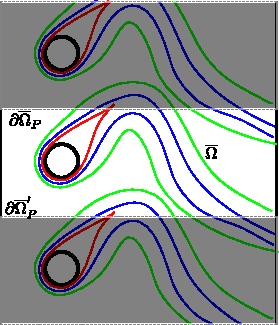
\includegraphics[width=0.4\linewidth]{periodic_bc.pdf}
\caption{Ячейка периодичности в задаче обтекания бесконечной решётки}
\label{fig:periodic_bc}
\end{figure}
На \figref{fig:periodic_bc} представлен пример области с выделенной ячейкой периодичности $\overline\Omega$ (незатенённая область).
Изолинии можно трактовать как изотермы решения задачи о нестационарном обтекании решётки нагревателя
(поле температур в этом случае описывается более сложным уравнением, чем \cref{eq:poissonnd_lam}
и приведено тут только для иллюстрации периодичности).

Пара периодических границ обозначена через $\partial\overline\Omega_P$ и $\partial\overline\Omega_P'$.
Пусть эти границы топологически экваивалентны, то есть для любой точки $\vec x\in\partial\overline\Omega_P$
cуществует взаимноодносзначная точка $\vec x'\in\partial\overline\Omega_P'$.
Для того, чтобы решение за этими границами точно соответствовало решению внутри ячейки периодичности необходимо
задать равенство значений и производных любого порядка:
\begin{equation}
\label{eq:poissonnd_bcp}
\left\{
\begin{array}{l}
    u(\vec x) = u(\vec x'), \\ [10pt]
    \left.\displaystyle\frac{\partial^k u}{\partial n^k}\right|_{\vec x} = -\left.\displaystyle\frac{\partial^k u}{\partial n^k}\right|_{\vec x'}
\end{array}
\right.
\vec x\in\partial\overline\Omega_P, \quad \vec x'\in\partial\overline\Omega_P', \quad \forall k.
\end{equation}
Здесь под $n$ подразумевается внешняя к ячейке периодичности нормаль, поэтому в правой части
условия для производных стоит минус.



\subsection{Метод конечных разностей}
Рассмотрим задачу \cref{eq:poissonnd,eq:poissonnd_bc} в упрощённой одномерной постановке:
\begin{equation}
    \label{eq:poisson1d}
    -\ddfrq{u}{x} = f(x)
\end{equation}
в области $x\in[a,b]$ с граничными условиями первого рода
\begin{equation}
	\label{eq:poisson1d_bc}
	\begin{cases}
        u(a)=u_a,\\[5pt]
        u(b)=u_b.\\
	\end{cases}
\end{equation}

Необходимо:
\begin{itemize}
\item 
	Запрограммировать расчётную схему для численного решения этого уравнения методом конечных разностей
	на сетке с постоянным шагом,
\item
	С помощью вычислительных экспериментов подтвердить порядок аппроксимации расчётной схемы.
\end{itemize}

\subsubsection{Метод решения}

\subsubsubsection{Нахождение численного решения}

В области решения $[a,b]$ введём равномерную сетку из $N$ ячеек.
Шаг сетки будет равен $h=(b-a)/N$.
Узлы сетки запишем в виде сеточного вектора $\{x_i\}$ длины $N+1$, где $i=\overline{0,N}$.
Определим сеточный вектор $\{u_i\}$ неизвестных, элементы которого определяют значение искомого численного решения в $i$-ом узле сетки. 

Разностная схема второго порядка для уравнения \eqref{eq:poisson1d} имеет вид
\begin{equation}
    \label{eq:poisson1d_fdm}
    \frac{-u_{i-1} + 2u_{i} - u_{i+1}}{h^2} = f_i, \qquad i=\overline{1,N-1}.
\end{equation}
Здесь $\{f_i\}$ -- известный сеточный вектор, определяемый через известную
аналитическую функцию $f(x)$ в правой части уравнения \eqref{eq:poisson1d} как
\begin{equation}
    \label{eq:poisson1d_fdm2}
    f_i = f(x_i).
\end{equation}

Аппроксимация граничных условий \eqref{eq:poisson1d_bc} первого рода даёт дополнительные 
сеточные уравнения для граничных узлов
\begin{equation}
    \label{eq:poisson1d_fdm_bc}
    \begin{array}{ll}
        u_0 = u_a,\\
        u_N = u_b
    \end{array}
\end{equation}

Линейные уравнения \eqref{eq:poisson1d_fdm}, \eqref{eq:poisson1d_fdm_bc}
составляют систему вида

\begin{equation*}
    \sum_{j=0}^{N} A_{ij}\,u_j = b_i, \qquad i=\overline{0,N}
\end{equation*}
с матричными коэффициентами
\begin{equation}
    \label{eq:poisson1d_fdm_lhs}
    A_{ij} = \begin{cases}
        1,      &\quad i=0, \, j=0; \\
        2/h^2,  &\quad i=\overline{1,N-1}, \, j=i;\\
        -1/h^2, &\quad i=\overline{1,N-1}, \, j=i-1;\\
        -1/h^2, &\quad i=\overline{1,N-1}, \, j=i+1;\\
        1,      &\quad i=N, \, j=N; \\
        0,      &\quad \text{иначе}.
    \end{cases}
\end{equation}
и правой частью
\begin{equation}
    \label{eq:poisson1d_fdm_rhs}
    b_i = \begin{cases}
        u_a,   &\quad i=0;\\
        u_b,   &\quad i=N;\\
        f_i,   &\quad i=\overline{1,N-1}.
    \end{cases}
\end{equation}
Искомый вектор находится путём решения этой системы.

\subsubsubsection{Практическое определения порядка аппроксимации}
\label{sec:compute-appr}

Порядок аппрокцимации показывает скорость
приближения численного решения к точному с уменьшением сетки.
Поэтому для подтверждения порядка необходимо
\begin{itemize}
\item Знать точное решение,
\item Уметь вычислять функционал (норму, $||\cdot||$), характеризующий отклонение точного решения от численного,
\item Сделать несколько расчётов на сетках с разной $N$  и заполнить таблицу $||\{u_i - u^e(x_i)\}||(N)$,
\item На основе этой таблицы построить график в логарифмических осях и по углу наклона кривой сделать вывод о порядке аппроксимации.
\end{itemize}

Выберем произвольную функцию $u^e$ (достаточно сильно изменяющуюся на целевом отрезке $[a,b]$).

Далее путём прямого вычисления определим параметры задачи $f$, $u_a$, $u_b$ такие,
для которых функция $u^e$ является точным решением задачи \eqref{eq:poisson1d}, \eqref{eq:poisson1d_bc}.

Зададимся числом разбиений $N$ и решим задачу для выбранным параметров.
В результате определим сеточный вектор численного решения $\{u_i\}$.

В качестве нормы выберем стандартное отклонение. В интегральном виде для многомерной функции $y(\vec x)$
в области $\vec x\in D$ оно имеет вид
\begin{equation}
    \label{eq:norm2_common}
    ||y(\vec x)||_2 = \sqrt{\frac{1}{|D|}\int_{D} y(\vec x)^2 \, d\vec x}.
\end{equation}
Упрощая до одномерного случая
\begin{equation*}
    ||y(x)||_2 = \sqrt{\frac{1}{b-a}\int_{a}^{b} y(x)^2 \, dx}.
\end{equation*}

Вычислим этот интеграл численно на введённой ранее равномерной сетке $\{x_i\}$:
\begin{equation*}
    ||\{y_i\}||_2 = \sqrt{\frac{1}{b-a}\sum_{i=0}^{N} w_i y_i^2},
\end{equation*}
где $\{w_i\}$ -- вес (или "площадь влияния") $i$-ого узла:
\begin{equation*}
    w_i = \begin{cases}
        h/2, &\quad i=0, N;\\
        h, &\quad i=\overline{1,N-1},
    \end{cases}
\end{equation*}
такая что
\begin{equation*}
    \sum_{i=0}^{N} w_i = b-a.
\end{equation*}

Окончательно среднеквадратичная норма отклонения численного решения от точного запишется в виде
\begin{equation}
    \label{eq:poisson1d_fdm_norm}
    ||\{u_i - u^e(x_i)\}||_2 = \sqrt{\frac{1}{b-a}\sum_{i=0}^{N} w_i \left(u_i - u^e_i\right)^2}.
\end{equation}

\subsubsection{Программная реализация}
\label{sec:poisson1d_prog}

\clisting{open}{"test/poisson_fdm_test.cpp"}

Тестовая программа для решения одномерного уравнения Пуассона 
реализована в файле \ename{poisson_fdm_solve_test.cpp}.

В качестве аналитической тестовой функции  используется
\begin{equation*}
    u^e = \sin(10 x^2)
\end{equation*}
на отрезке $x\in[0,1]$.

\subsubsubsection{Функция верхнего уровня}
объявлена как
\clisting{line}{", \"[poisson1-fdm]\")"}
В программе в цикле по набору разбиений \cvar{n_cells}
\clisting{line}{"for (size_t n_cells"}
создаётся решатель для тестовой задачи, использующий заданное число ячеек
\clisting{line}{"worker"}
вычисляется среднеквадратичная норма отклонения численного решения от точного
\clisting{line}{"n2"}
полученное численное решение (вместе с точным) сохраняется в vtk файле\\
\ename{poisson1_n={10,20,...}.vtk}
\clisting{line}{"save_vtk"}
а полученная норма печатается в консоль напротив количества ячеек
\clisting{line}{"cout"}

В результате работы программы в консоли должна отобразиться таблица вида
\begin{shelloutput}
--- [poisson1] ---
10 0.179124
20 0.0407822
50 0.00634718
100 0.00158055
200 0.000394747
500 6.31421e-05
1000 1.57849e-05
\end{shelloutput}
где первый столбец -- это количество ячеек, а второй -- полученная для этого количества ячеек норма.
Нарисовав график этой таблицы в логарифмических осях подтвердим второй порядок аппроксимации (\figref{fig:poisson_convergence}).

\begin{figure}[h]
\centering
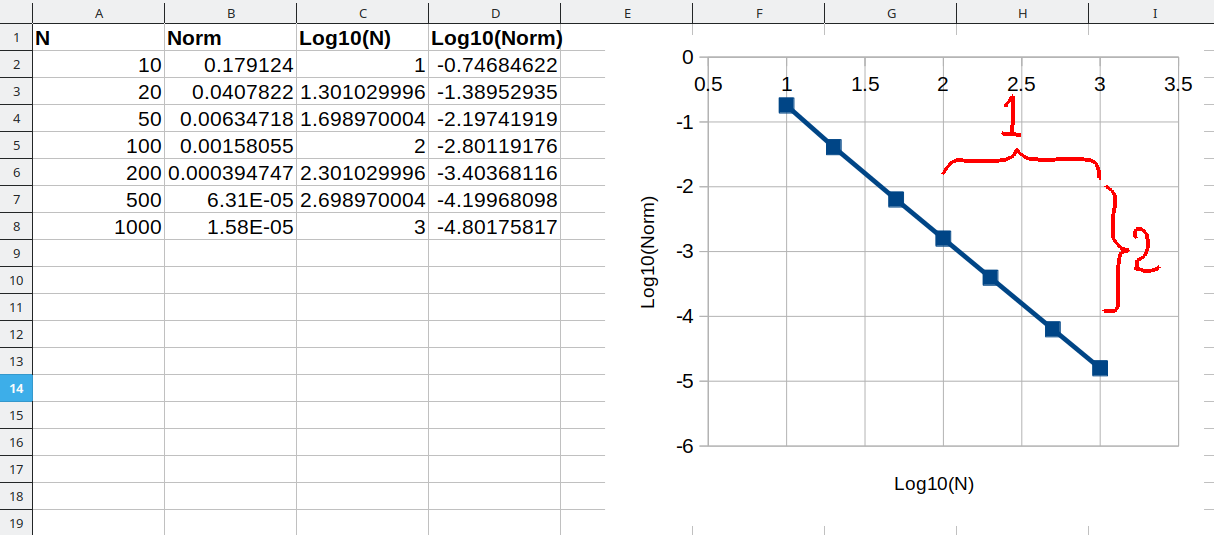
\includegraphics[width=0.9\linewidth]{poisson1_appr.png}
\caption{Сходимость с уменьшением разбиения при решении одномерного уравнения Пуассона}
\label{fig:poisson_convergence}
\end{figure}

Открыв один из cохранённых в процессе работы файлов vtk \ename{poisson1_ncells=?.vtk} в paraview
можно посмотреть полученные графики. В файле представлены как точное ``exact'', так и численное решение ``numerical''
(\figref{fig:poisson_graph}).

\begin{figure}[h]
\centering
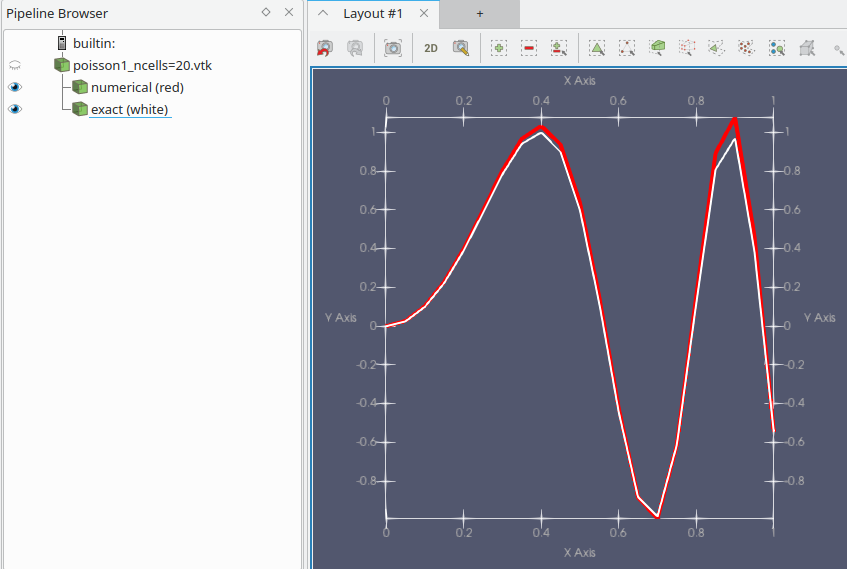
\includegraphics[width=0.9\linewidth]{poisson1_graph.png}
\caption{Сравнение точного и численного решений уравнения Пуассона}
\label{fig:poisson_graph}
\end{figure}


\subsubsubsection{Детали реализации}
\clisting{open}{"test/poisson_fdm_test.cpp"}
Основная работа по решению задачи проводится в классе \cvar{TestPoisson1Worker}.

В его конструкторе происходит инициализация сетки (приватного поля класса) на отрезке $[0, 1]$ с заданным разбиением
\cvar{n_cells}:
\clisting{line}{"TestPoisson1Worker"}

В методе \cvar{solve()} производится численное решения задачи и вычисления нормы.
Для этого последовательно
\begin{enumerate}
\item Строится матрица левой части и вектор правой части определяющей системы уравнений.
      Матрицы хранятся в разреженном формате CSR (\secref{sec:csr}), удобном для последовательного чтения.
\item Вызывается решатель СЛАУ. Решение записывается в приватное поле класса \cvar{u}.
\item Вызывается функция вычисления нормы.
\end{enumerate}

\clisting{block}{"double solve()"}

Функции нижнего уровня (используемые в методе \cvar{solve}):
\begin{itemize}
\item
  Сборка левой части СЛАУ. Реализует формулу \eqref{eq:poisson1d_fdm_lhs}.
  Для заполнения матрицы используется формат \cvar{cfd::LodMatrix} (\secref{sec:lodmat}), удобный для непоследовательной записи, который в конце конвертируется CSR.
  \clisting{block}{"approximate_lhs("}
\item
  Сборка правой части СЛАУ. Реализует формулу \eqref{eq:poisson1d_fdm_rhs}.
  \clisting{block}{"approximate_rhs("}
\item
  Вычисление нормы. Реализует формулу \eqref{eq:poisson1d_fdm_norm}.
  \clisting{block}{"compute_norm2"}
\end{itemize}

\subsection{Метод конечных объёмов}
\label{sec:FVM}
Будем рассматривать задачу в многомерной постановке \cref{eq:poissonnd,eq:poissonnd_bc}.

\subsubsection{Конечнообъёмная сетка}
Разобъём oбласть численного решения на непересекающиеся подобласти $E_i$, $i = \overline{0, N-1}$,
а её границу $\partial \Omega$ на грани $\Gamma_s$, $s = \overline{0, N^\Gamma - 1}$ (\figref{fig:fvm_grid}).
Введем следующие сеточные примитивы:
\begin{itemize}
\item $E_i$ -- ячейка сетки,
\item $\Gamma_{s}$ -- граничная грань,
\item $\vec c_i$ -- центр (масс) ячейки,
\item $\vec g_s$ -- центр (масс) грани $\Gamma_{s}$,
\item $\gamma_{ij}$ -- внутренняя грань между $i$-ой и $j$-ой ячейками,
\end{itemize}
Будем считать, что ячейки сетки выпуклые, а грани -- плоские.

\begin{figure}[h!]
\centering
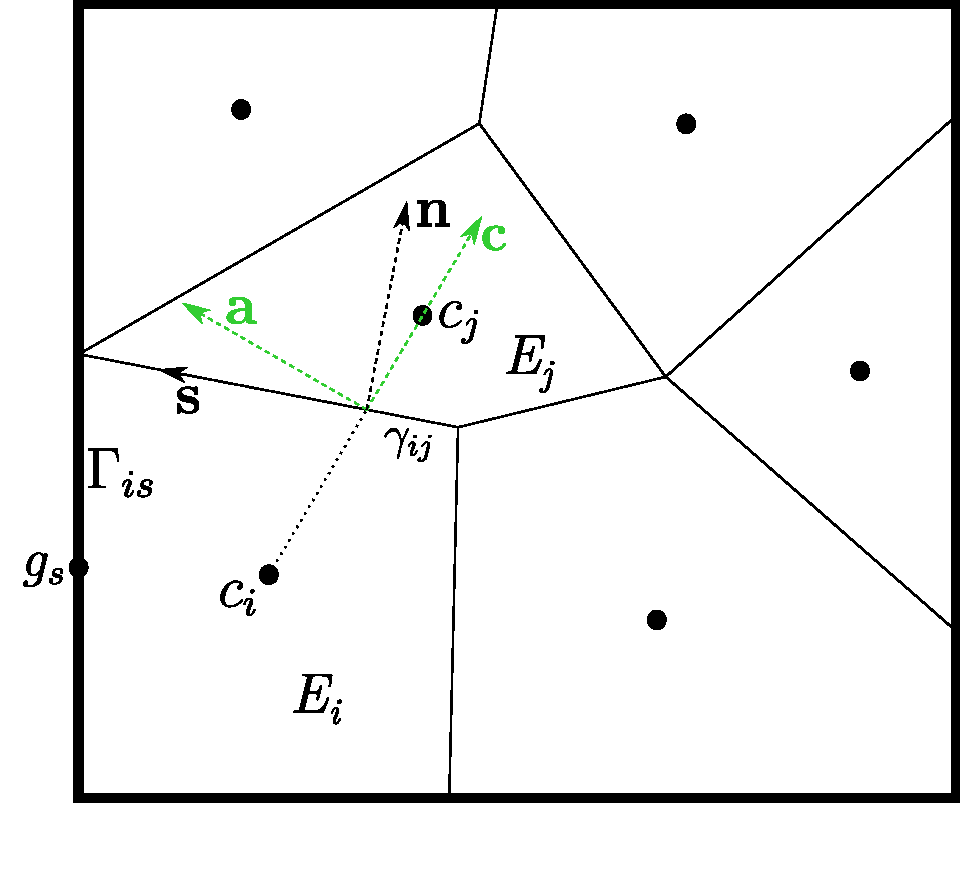
\includegraphics[width=0.4\linewidth]{fvm_grid.pdf}
\caption{Конечнообъёмная сетка}
\label{fig:fvm_grid}
\end{figure}

\subsubsection{Конечнообъёмная аппроксимация}
\label{sec:fvm_appr}

Проинтегрируем исходное уравнение по одной из подобластей $E_i$:
\begin{equation*}
-\arint{\nabla^2 u}{E_i}{s} = \arint{f}{E_i}{\vec x}.
\end{equation*}
К интегралу в левой части применим формулу интегрирования по частям \cref{eq:partint_laplace}. Получим
\begin{equation}
\label{eq:fvm_pois_int}
-\arint{\dfr{u}{n}}{\partial E_i}{\vec x} = \arint{f}{E_i}{\vec x}.
\end{equation}
Здесь $\partial E_i$ -- совокупность всех границ подобласти $E_i$,
а $\vec n$ -- внешняя к подобласти нормаль.

Граница ячейки $E_i$ состоит из внутренних граней $\gamma_{ij}$ (индекс $j$ здесь
соответствует индексу соседней ячейки)
и инцидентных ей граней $\Gamma_{s}$, лежащих на внешней границе расчётной области $\Omega$.
Тогда интеграл по общей границе ячейки распишется через сумму интегралов по плоским поверхностям
$$
\arint{\dfr{u}{n}}{\partial E_i}{s} = \sum_{j\in{{\rm J}_i}}\arint{\dfr{u}{n}}{\gamma_{ij}}{s} + \sum_{s\in{\rm I}_i}\arint{\dfr{u}{n}}{\Gamma_{s}}{s}.
$$
Введены следующие обозначения множества индексов: ${\rm J}_i$ -- индексы ячеек, соседних (имеющих общую грань) с текущей ячейкой $i$,
${\rm I}_i$ -- индексы граничных граней первого рода, инцидентных ячейке $E_i$.
Аппроксимирум производную $\dsfr{u}{n}$ на каждой из граней константой.
Тогда её можно вынести из под интегралов и предыдущее выражение записать в виде
\begin{equation}
\label{eq:fvm_gamma_integral}
\arint{\dfr{u}{n}}{\partial E_i}{s} \approx
\sum_{j\in{{\rm J}_i}}
    \left|
        \gamma_{ij}
    \right|
    \left(
        \dfr{u}{n}
    \right)_{\gamma_{ij}}
+\sum_{s\in{{\rm I}_i}}
    \left|
        \Gamma_{s}
    \right|
    \left(
        \dfr{u}{n}
    \right)_{\Gamma_{s}}
\end{equation}

Аналогично, анализируя интеграл правой части \cref{eq:fvm_pois_int},
приблизим значение функции правой части $f$ внутри элемента $E_i$ константой $f_i$,
которую отнесём к центру элемента. Тогда
\begin{equation}
\label{eq:fvm_f_integral}
\arint{f}{E_i}{\vec x} \approx f_i \left|E_i\right|.
\end{equation}

Сеточный вектор $\{f_i\}$ -- есть конечнообъёмная аппроксимация
функции $f(\vec x)$ на конечнообъёмную сетку.
Значения $f_i$ при аппроксимации чаще всего находятся как значения в центрах элементов
$$
f_i = f(\vec c_i).
$$
Хотя иногда может быть использовано и другое определение,
следующее из \eqref{eq:fvm_f_integral}:
$$
f_i = \frac{1}{\left| E_i \right|} \arint{f(\vec x)}{E_i}{\vec x}.
$$


\subsubsubsection{Обработка внутренних граней}
Для начала будем рассматривать сетки, в
которых вектора $\vec c$, соединяющие центры ячеек (зедёные вектора на \figref{fig:fvm_grid}),
коллинеарны (или почти коллинеарны) нормалям к граням $\vec n$.
В этом случае производную искомой функции по нормали к грани можно записать в виде
$$
\dfr{u}{n} = \dfr{u}{c}.
$$

Далее определим значения функции $u$ в точках $c_i$, $c_j$ как $u_i$, $u_j$.
Тогда значение производной $\dsfr{u}{n}$ на внутренней грани конечного объёма
может быть приближена конечной разностью
\begin{equation}
\label{eq:fvm_dudn_dudc}
\left(\dfr{u}{n}\right)_{\gamma_{ij}} \approx \dfr{u}{c} \approx \frac{u_j - u_i}{h_{ij}}, \quad h_{ij} = |\vec c_j - \vec c_i|.
\end{equation}

Определим pebi (perpendicular-bisector) сетки как сетки, удовлетворяющие следующим свойствам
\begin{itemize}
\item линии, соединяющие центры двух соседних ячеек, перпендикулярны грани между этими ячейками;
\item внутренние грани делят линии, соединящие центры соседних ячеек, пополам.
\end{itemize}
Очевидно, что равномерная структурированная сетка удовлетворяет этим свойствам.
Для построения неструктурированных pebi-сеток используют алгоритмы построения ячеек Вороного.
Для pebi-сеток разностная схема \eqref{eq:fvm_dudn_dudc}
является симметричной разностью и, поэтому, имеет второй порядок аппроксимации.

\subsubsubsection{Учёт граничных условий первого рода}
Для вычисления второго слагаемого в правой части 
\cref{eq:fvm_gamma_integral}
следует расписать значение нормальной 
к границе производной вида
$$
\left(\dfr{u}{n}\right)_{\Gamma_{s}}.
$$
Это делается с помощью граничных условий.

Пусть в центре $\vec g_s$ грани $\Gamma_{s}$ задано 
значение искомой функции \cref{eq:poissonnd_bc}:
\begin{equation}
\label{eq:fvm_bc1}
u(\vec g_s) = u^\Gamma_s.
\end{equation}
Аппроксимацию производных
будем проводить из тех же соображений, которые использовали
при анализе внутренних граней. Только вместо центра соседнего элемента
$c_j$ будем использовать центр грани $g_s$.
В первом приближении, отбрасывая касательные производные, придём к формуле, аналогичной \cref{eq:fvm_dudn_dudc}:
\begin{equation}
\label{eq:fvm_bc1_approx}
\left(\dfr{u}{n}\right)_{\Gamma_s} \approx \frac{u^\Gamma_s - u_i}{h^\Gamma_{is}}, \quad h^\Gamma_{is} = \left| \vec g_s  - \vec c_i \right|.
\end{equation}

\subsubsection{Одномерный случай}
Рассмотрим результат конечнообъёмной аппроксимации
задачи \cref{eq:poissonnd} в одномерном случае \cref{eq:poisson1d}
на равномерной сетке с шагом $h$ (\figref{fig:fvm_grid1d}).

\begin{figure}[h!]
\centering
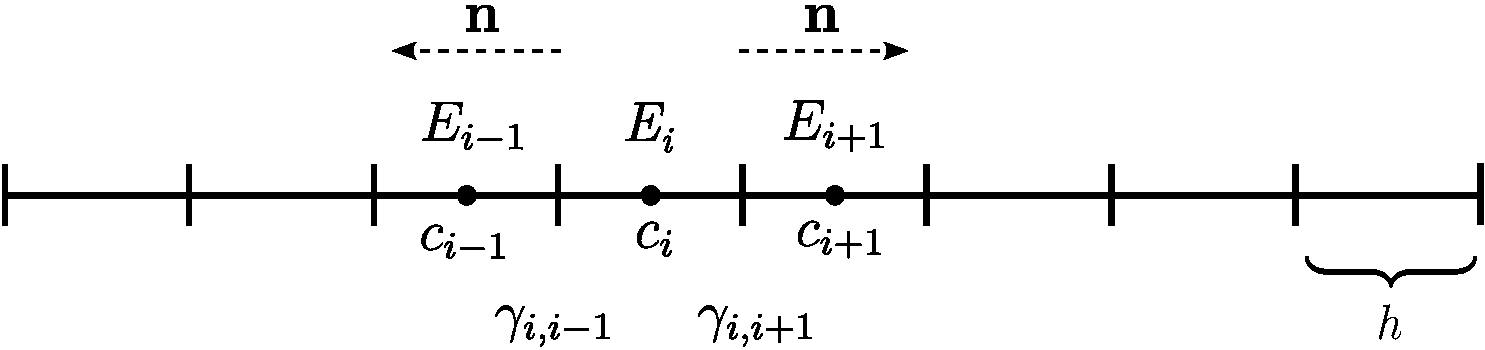
\includegraphics[width=0.6\linewidth]{fvm_grid1d.pdf}
\caption{Одномерная конечнообъёмная сетка}
\label{fig:fvm_grid1d}
\end{figure}

У внутренней ячейки $i$ есть две границы: $\gamma_{i,i-1}$ и $\gamma_{i,i+1}$.
Нормали по этим границам аппроксимируются по формулам \cref{eq:fvm_dudn_dudc}:
\begin{align*}
\gamma_{i,i-1}: \quad& \dfr{u}{n} = \frac{u_{i-1}-u_{i}}{h} \\[10pt]
\gamma_{i,i+1}: \quad& \dfr{u}{n} = \frac{u_{i+1}-u_{i}}{h}
\end{align*}
Объём ячейки в одномерном случае равен её длине $h$.
Площадь грани следует положить единице с тем, чтобы
$$
|E_i| = |\gamma| h = h.
$$
Тогда, подставляя эти значения в \cref{eq:fvm_pois_int},
получим знакомую конечноразностную схему аппроксимацию уравнения Пуассона
$$
\frac{-u_{i-1} + 2 u_i - u_{i+1}}{h} = f_i h,
$$
которая имеет второй порядок точности.
Разница с методом конечных разностей здесь состоит в том,
что значения сеточных векторов $\gvec{u}$, $\gvec{f}$ здесь
приписаны к центрам ячеек, а не к их узлам.
Это отличие проявит себя в аппроксимации граничных условий.
Так, если на левой границе $x=a$ задано условие первого рода, то соответствующее уравнение
согласно \cref{eq:fvm_bc1_approx}
примет вид
$$
-\frac{u^\Gamma_a - u_0}{h/2} - \frac{u_1 - u_0}{h} = f_0 h.
$$
В методе конечных разностей это условие выразилось бы в виде $u_0 = u^\Gamma_a$.

\subsubsection{Сборка системы линейных уравнений}
Подставим все полученные аппроксимации
\cref{eq:fvm_dudn_dudc,eq:fvm_bc1_approx}
в уравнение \cref{eq:fvm_pois_int}. Получим $i$-ое уравнение искомой системы уравнений относительно неизвестных $u_i$:
\begin{equation*}
-\sum_{j\in {\rm J}_i}
    \frac{|\gamma_{ij}|}{h_{ij}}
         \left(u_j - u_i\right)
-\sum_{s\in{\rm I}_i}
    \frac{|\Gamma_{s}|}{h^\Gamma_{is}}
        \left(u^\Gamma_s - u_i\right)
=
f_i |E_i|.
\end{equation*}
Здесь первое слагаемое в левой части отвечает за потоки через внутренние границы,
второе -- граничные условия первого рода.
Далее перенесём все известные значения в правую часть и окончательно
получим линейное уравнение для $i$-го конечного объёма:
\begin{equation}
\label{eq:fvm_slae}
\sum_{j\in{\rm J}_i}
    \frac{|\gamma_{ij}|}{h_{ij}}
         \left(u_i - u_j\right)
+\sum_{s\in{\rm I}_i}
    \frac{|\Gamma_{s}|}{h^\Gamma_{is}}u_i
 =
f_i |E_i|
+\sum_{s\in{\rm I}_i}
    \frac{|\Gamma_{s}|}{h^\Gamma_{is}} u_s^\Gamma
\end{equation}
Таким образом мы получили систему из $N$ (по количеству подобластей) линейных уравнений относительно
неизвестного сеточного вектора $\left\{u_i\right\}$
$$
A u = b.
$$

Полученные в результате сборочных процедур матрицы являются разреженными -- то есть большинство их элементов равно нулю.
Полное хранение таких матриц в памяти невозможно, поэтому применяют специальные процедуры разреженного хранения (см. \secref{sec:sparse-matrix}).

Ниже приведён псеводкод для сборки СЛАУ. Перед началом процедур сборки левую правую часть нужно инициализировать нулями.

\subsubsubsection{Алгоритм сборки в цикле по ячейкам}
\label{sec:poisson_fvm_cellbased}
Матрицу $A$ и правую часть $b$ системы \cref{eq:fvm_slae} можно
собирать в цикле по ячейкам: строчка за строчкой.
Такой алгоритм выглядел бы следующим образом
\begin{equation*}
\begin{array}{ll}
\textbf{for } i = \overline{0, N-1}                          & \textrm{-- цикл по строкам СЛАУ}\\
\qquad b_i = |E_i| f_i                                       & \\
\qquad \textbf{for } j \in \textrm{nei(i)}                   & \textrm{-- цикл по ячейкам, соседним с ячейкой $i$}\\
\qquad \qquad v = \sfrac{|\gamma_{ij}|}{h_{ij}}              & \\
\qquad \qquad A_{ii} \pluseq v                               & \\
\qquad \qquad A_{ij} \minuseq v                              & \\
\qquad \textbf{endfor}                                       & \\
\qquad \textbf{for } s \in \textrm{bnd1(i)}                  & \textrm{-- цикл по граням ячейки $i$ с условиями первого рода}\\
\qquad \qquad v = \sfrac{|\Gamma_{s}|}{h^\Gamma_{is}}        & \\
\qquad \qquad A_{ii} \pluseq v                               & \\
\qquad \qquad b_{i}  \pluseq u_s^{\Gamma} v                  & \\
\qquad \textbf{endfor}                                       & \\
\textbf{endfor}
\end{array}
\end{equation*}
Первым недостатком такого алгоритма является наличие вложенных циклов.
Во-вторых, коэффициент, отвечающий за поток через внутреннюю грань $\gamma_{ij}$,
равный $\sfrac{|\gamma_{ij}|}{h_{ij}}$ в таком алгоритме будет учитываться дважды:
в строке $i$ и в строке $j$.

\subsubsubsection{Алгоритм сборки в цикле по граням}
\label{sec:poisson_fvm_facebased}
Вместо общего цикла по ячейкам, будем использовать цикл по граням.
В таком цикле коэффициенты потоков будут вычисляться один раз
и вставляться сразу в две строки матрицы, соответствующие соседним с гранью ячейкам.
Вложенных циклов в такой постановке удаётся избежать, потому
что у грани есть только две соседние ячейки (в то время как у ячейки может быть произвольное
количество соседних граней).

Разделим все грани на исходной сетки на внутренние и граничные (отдельный набор для каждого вида граничных условий).
Тогда для внутренних граней можно записать
\begin{equation}
\label{eq:fvm_assem_internal}
\begin{array}{ll}
\textbf{for } s \in\textrm{internal}                     & \textrm{-- цикл по внутренним граням}\\ 
\qquad i,j = \textrm{nei\_cells(s)}                      & \textrm{-- две ячейки, соседние с текущей гранью}\\
\qquad v = \sfrac{|\gamma_{ij}|}{h_{ij}}                 & \\
\qquad A_{ii} \pluseq  v; \quad A_{jj} \pluseq  v        & \textrm{-- диагональные коэффициенты матрицы}\\ 
\qquad A_{ij} \minuseq v; \quad A_{ji} \minuseq v        & \textrm{-- внедиагональные коэффициенты матрицы}\\
\textbf{endfor}                                          & \\
\end{array}
\end{equation}
Граничные условия учитываются в отдельных циклах.
Здесь будем учитывать, что у грани, принадлежащей
границе области, есть только одна соседняя ячейка.
Условия первого рода:
\begin{equation}
\label{eq:fvm_assem_bc1}
\begin{array}{ll}
\textbf{for } s \in\textrm{bnd1}                         & \textrm{-- грани с условиями первого рода}\\ 
\qquad i = \textrm{nei\_cell(s)}                         & \textrm{-- соседняя с граничной гранью ячейка}\\
\qquad v = \sfrac{|\Gamma_{s}|}{h^\Gamma_{is}}           & \\
\qquad A_{ii} \pluseq  v                                 & \\ 
\qquad b_{i} \pluseq u_s^\Gamma v                        & \\
\textbf{endfor}                                          & \\
\end{array}
\end{equation}
Первое слагаемое в правой части
\cref{eq:fvm_slae}
учтём отдельным циклом:
\begin{equation}
\label{eq:fvm_assem_f}
\begin{array}{ll}                                         & \\
\textbf{for } i = \overline{0,N-1}                        & \textrm{-- цикл по ячейкам}\\ 
\qquad b_i \pluseq |E_i| f_i                              & \\
\textbf{endfor}                                           &
\end{array}
\end{equation}

\subsubsection{Расширенный набор точек коллокаций}
\label{sec:poisson_fvm_extended_facebased}
До сих пор мы соотносили
элементы сеточных векторов, которые получаются при аппроксимации функции на конечнообъёмную сетку,
с центрами конечных объёмов.
То есть точками коллокации служили центры объёмов,
а длина сеточных векторов (количество точек коллокации)
равнялась количеству ячеек сетки.
Для написания аппроксимационных соотношений около границ будет удобно расширить набор точек коллокаций за счёт
центров граничных граней.

Такой подход позволяет универсализировать подходы
к аппроксимации перетоков через грани.
То есть для каждой грани вмеcто использования разных алгоритмов для внутренних \cref{eq:fvm_assem_internal} и граничных \cref{eq:fvm_assem_bc1} граней, нужно использовать универсальный алгоритм
\begin{equation}
\label{eq:fvm_assem_bc_extended}
\begin{array}{ll}
\textbf{for } s \in\overline{0, N_f - 1}            & \textrm{-- цикл по всем граням}\\
\qquad i,j = \textrm{nei\_colloc(s)}                & \textrm{-- инцидентные точки коллокаций}\\
\qquad v = \sfrac{|\gamma_{ij}|}{h_{ij}}            & \\
\qquad A_{ii} \pluseq  v, \quad A_{ij} \minuseq v   & \textrm{-- $i$-ая строка}\\ 
\qquad A_{jj} \pluseq  v, \quad A_{ji} \minuseq v   & \textrm{-- $j$-ая строка}\\ 
\textbf{endfor}                                     & \\
\end{array}
\end{equation}
Отметим, что эта процедура заполняет не только строки, соответствующие внутренним коллокациям, но и строки для граничных точек.
Последние заполняются выражениями, соответствующие интегралам от нормальных производных
\begin{equation*}
-\arint{\dfr{u}{n}}{\Gamma_s}{s} \approx -\left.\dfr{u}{n}\right|_{\vec{g}_s} |\Gamma_s|\
\approx \frac{u^\Gamma_s - u_j}{h^\Gamma_{is}} |\Gamma_s|,
\end{equation*}
где $i$ -- индекс ячейки, соседний с гранью $\Gamma_s$.
Для задач с граничными условиями первого рода эти строки излишни и будут переписаны, но они окажутся
полезными позднее, при учёте других типов граничных условий.

Строки матрицы, соответствующие граничным точкам коллокации,
будут содержеть аппроксимированные граничные условия.
Так, для граней с условиями первого рода будет аппроксимироваться непосредственно выражение
\cref{eq:fvm_bc1}. Алгоритмическом виде это примет вид
\begin{equation}
\label{eq:fvm_assem_bc1_extended}
\begin{array}{ll}
\textbf{for } s \in\textrm{bnd1}                         & \textrm{-- грани с условиями первого рода}\\ 
\qquad j = \textrm{bnd\_col(s)}                          & \textrm{-- индекс точки коллокации, соответствующей грани}\\
\qquad A_{ij} = \delta_{ij}                              & \textrm{-- единичная диагональ}\\ 
\qquad b_{j} = u^\Gamma_s                                & \\
\textbf{endfor}                                          & \\
\end{array}
\end{equation}

Преимуществами такого подхода является:
\begin{itemize}
\item Более очевидный учёт граничных условий в отдельной строке СЛАУ,
\item Наличие явно выраженного граничного значения функции в сеточном векторе.
\end{itemize}

\subsubsubsection{Пример}
\begin{figure}[h]
\centering
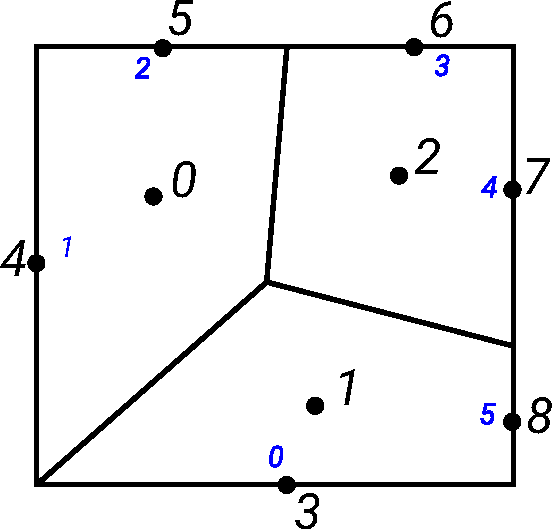
\includegraphics[width=0.25\linewidth]{extended_coll.pdf}
\caption{Расширенный набор точек коллокации}
\label{fig:extended_coll}
\end{figure}

На рис.~\ref{fig:extended_coll}.
представлена конечнообъёмная сетка, содержащая три ячейки
и девять граней. Индексация граничных граней обозначена синими цифрами.
Согласно стандартной методике конечных
объёмов сеточная функция
будет представлена массивом из трёх элементов.
В расширенном наборе будет девять точек коллокации (обозначены чёрными кругами и проиндексированы чёрными цифрами):
три соответствуют центрам ячеек и ещё шесть -- центрам граничных граней.

Пусть в области с рис.~\ref{fig:extended_coll} нужно решить
уравнение Пуассона \cref{eq:poissonnd}.
Пусть на нижней и правой гранях задано условие первого рода: $u = C$.

\paragraph{Классический подход}
Согласно классическому методу конечных объёмов
(\secref{sec:poisson_fvm_facebased})
аппроксимация задачи в ячейке с индексом 1 будет иметь следующий вид
$$
\frac{u_1 - u_0}{h_{10}}|\gamma_{10}|
+\frac{u_1 - u_2}{h_{12}}|\gamma_{12}|
+\frac{u_1 - C}{h^\Gamma_{10}}|\Gamma_0|
+\frac{u_1 - C}{h^\Gamma_{15}}|\Gamma_5|
= |E_1| f_1.
$$
Общая размерность матрицы СЛАУ при таком подходе будет
равна $3\times3$, а её элементы в 1-ой строке равны
$$
a_{10} = -\frac{|\gamma_{10}|}{h_{10}},  \quad
a_{12} = -\frac{|\gamma_{12}|}{h_{12}},  \quad
a_{11} = \frac{|\gamma_{10}|}{h_{10}}  + \frac{|\gamma_{12}|}{h_{12}} + \frac{|\Gamma_{0}|}{h^\Gamma_{10}} + \frac{|\Gamma_5|}{h^\Gamma_{15}}.
$$
Справа в 1-ой строке будет стоять
$$
b_1 = |E_1| f_1 + \frac{C |\Gamma_0|}{h^\Gamma_{10}} + \frac{C |\Gamma_5|}{h^\Gamma_{15}}.
$$

\paragraph{Новый подход}
В расширенным набором точек коллокаций
матрица правой части будет иметь размерность $9\times9$.
Из них первые три будут собираться согласно классической процедуре
метода конечных объёмов, но учитывая наличие дополнитиельных точек коллокации в центрах
граничных граней. Так, 1-ое уравнение итоговой СЛАУ, собранной согласно процедуре из
\secref{sec:poisson_fvm_extended_facebased},
примет вид
$$
\frac{u_1 - u_0}{h_{10}}|\gamma_{10}|
+\frac{u_1 - u_2}{h_{12}}|\gamma_{12}|
+\frac{u_1 - u_3}{h_{13}}|\gamma_{13}|
+\frac{u_1 - u_8}{h_{18}}|\gamma_{18}|
= |E_1| f_1.
$$
Здесь введено соотвествие для граничных граней и расстояний:
$$
\gamma_{13} = \Gamma_0, h_{13} = h^\Gamma_{10}, \gamma_{18} = \Gamma_5, h_{18} = h^\Gamma_{15}.
$$
Остальные шесть уравнений будут представлять из себя
аппроксимацию граничных условий для соответствующих граней.
Так, 3-е и 8-е уравнение будет соответствовать условию первого рода:
$$
u_3 = C, \qquad u_8 = C.
$$
Переводя рассмотренные уравнения в матричные коэффициенты, получим
следующие ненулевые коээфиициенты итоговой матрицы $\{a_{ij}\}$ и вектора правой части $\{b_i\}$. Для 1-ой строки
$$
a_{10} = -\frac{|\gamma_{10}|}{h_{10}},  \quad
a_{12} = -\frac{|\gamma_{12}|}{h_{12}},  \quad
a_{13} = -\frac{|\gamma_{13}|}{h_{13}},  \quad
a_{18} = -\frac{|\gamma_{18}|}{h_{18}},  \quad
a_{11} = a_{10} + a_{12} + a_{13} + a_{18}, \quad
b_1 = |E_1| f_1,
$$
для 3-ей строки
$$
a_{33} = 1, \quad b_3 = C,
$$
для 8-ой строки
$$
a_{88} = 1, \quad b_8 = C.
$$

\subsubsection{Граничные условия второго рода}
Рассмотрим участок границы $\partial\Omega_{II}$ на котором заданы условия второго рода
\cref{eq:poissonnd_bc2} при $\lambda=1$.
Проинтегрируем это условие по грани и получим уравнение для граничного узла коллокации:
\begin{equation*}
-\arint{\dfr{u}{n}}{\Gamma_s}{s} = \arint{q(s)}{\Gamma_s}{s} \approx |\Gamma_s| q(\vec g_s).
\end{equation*}
При сборке матрицы левой части согласно процедуре
\cref{eq:fvm_assem_bc_extended} левая часть этого уравнения уже содержит
интеграл от нормальной производной.
Тогда алгоритм сборки этого условия будет включать в себя только подстановку $q$ в правую часть:
\begin{equation}
\label{eq:fvm_assem_bc2_extended}
\begin{array}{ll}
\textbf{for } s \in\textrm{bnd2}                         & \textrm{-- грани с условиями второго рода}\\ 
\qquad j = \textrm{bnd\_col(s)}                          & \textrm{-- индекс точки коллокации, соответствующей грани}\\
\qquad b_{j} = |\Gamma_s| q(\vec g_s)                    & \\
\textbf{endfor}                                          & \\
\end{array}
\end{equation}

\subsubsection{Граничные условия третьего рода}
Теперь рассмотрим участок границы $\partial\Omega_{III}$ с условиями
\cref{eq:poissonnd_bc3} при $\lambda=1$.
Так же проинтегрируем его по $s$-ой грани
\begin{equation*}
-\arint{\dfr{u}{n}}{\Gamma_s}{s} = \arint{\alpha(s) u + \beta(s)}{\Gamma_s}{s} \approx |\Gamma_s| \left(\alpha(\vec g_s) u_s + \beta(\vec g_s)\right).
\end{equation*}
Перенесём слагаемое с неизвестной $u_s$ в левую часть (то есть добавим коэффициент в диагональ матрицы), а $\beta$ оставим справа.
Тогда, после сборки матрицы левой части по процедуре 
\cref{eq:fvm_assem_bc_extended}, модифицируем матрицу и правую часть следующим образом:
\begin{equation}
\label{eq:fvm_assem_bc3_extended}
\begin{array}{ll}
\textbf{for } s \in\textrm{bnd3}                         & \textrm{-- грани с условиями третьего рода}\\ 
\qquad j = \textrm{bnd\_col(s)}                          & \textrm{-- индекс точки коллокации, соответствующей грани}\\
\qquad A_{jj} \pluseq |\Gamma_s| \alpha(\vec g_s)             & \\
\qquad b_{j} = |\Gamma_s| \beta(\vec g_s)                & \\
\textbf{endfor}                                          & \\
\end{array}
\end{equation}

\subsubsection{Периодические граничные условия}
Рассмотрим периодическую пару границ $\partial\Omega_{P}$, $\partial\Omega_{P}'$.
Для того, чтобы такое условие можно было аппроксимировать сеточным методом,
необходимо, чтобы сетка на границе $\partial\Omega_P$ в точности соотвествовала сетке на границе $\partial\Omega_P'$.

Естественный способ удовлетворить граничные уловия вида
\cref{eq:poissonnd_bcp} -- модифицировать таблицы связности сетки так, чтобы грани, лежащие на этих границах перестали быть граничными.
То есть нужно убрать граничные точки коллокации, и добавить запись в таблицы связности \quo{грань-ячейка}.
Такая процедура требует специальной подстройки сеточных таблиц.

Чтобы этого избежать, можно работать без модификации сетки, но удовлетвормить формальным математическим условиям \cref{eq:poissonnd_bcp}.
Поскольку конечнообъёмная аппроксимация уравнения Пуассона имеет не более чем второй порядок точности, достаточно записать это условие только для первой производной.
Для периодической пары граничных граней с индексами $s$ и $s'$ это условие можно записать следующим образом:
\begin{align}
\label{eq:periodic_for_fem_poisson_1}
&u(\vec g_s) - u(\vec g_{s'}) = 0, \\
\label{eq:periodic_for_fem_poisson_2}
&-\arint{\dfr{u}{n}}{\Gamma_s}{s} - \arint{\dfr{u}{n}}{\Gamma_{s'}}{s} = 0.
\end{align}

Первое из этих условий условий запишем в строке, соответствующей грани $s$, а второе - в строке для грани $s'$.
При сборке \cref{eq:periodic_for_fem_poisson_2} учтём, что предворительно проведённая процедура
\cref{eq:fvm_assem_bc_extended}
собирает входящие в него пару интегралов в строках для грани $s$ и $s'$ соответсвенно.
Чтобы записать сумму этих интегралов, нужно просто суммировать эти строки матрицы.
Тогда процедура примет следующий вид

\begin{equation}
\label{eq:fvm_assem_bcp_extended}
\begin{array}{ll}
\textbf{for } s,s' \in\textrm{periodic\_pairs}           & \textrm{-- периодические пары граней}\\ 
\qquad i,j = \textrm{bnd\_col(s, s')}                    & \textrm{-- индексы граничных точек коллокации}\\
\qquad \textbf{for } k \in \overline{0, N+N^\Gamma-1}    & \textrm{-- цикл по столбцам}\\
\qquad\qquad  A_{jk} \pluseq A_{ik}                      & \textrm{-- складываем строки $i+j$ \cref{eq:periodic_for_fem_poisson_1}}\\
\qquad\qquad A_{ik} = 0                                  & \textrm{-- зануляем строку $i$}\\
\qquad \textbf{endfor}                                   & \\
\qquad A_{jj} \pluseq A_{ji}, \quad A_{ji} = 0           & \textrm{-- усилим диагональ $A_{jj}$ (т.к $u_i = u_j$)}\\
\qquad A_{ii} = 1, \quad A_{ij} = -1                     & \textrm{-- удовлетворим \cref{eq:periodic_for_fem_poisson_2}}\\
\textbf{endfor}                                          & \\
\end{array}
\end{equation}

\subsubsection{Учёт неортогональности сетки}
\label{sec:nonortho_fvm}
Конечнообъёмная схема, описываемая уравнениями \cref{eq:fvm_pois_int,eq:fvm_gamma_integral},
не использует в своем выводе аппроксимационных соотношений, и поэтому является точной.
Погрешность аппроксимации вносится при расписывании нормальных производных на грани
по разностным формулам: \cref{eq:fvm_dudn_dudc,eq:fvm_bc1_approx} через значения скалярной функции в точках коллокации.
Эти формулы имеют второй порядок аппроксимации в случае
ортогональных сеток. Поэтому для таких сеток
вся конечнообъёмная схема имеет второй порядок аппроксимации.
Но если в сетке присутствуют скошенные ячейки,
такие разностные соотношения дают только порядок точности.
Чтобы сохранить второй порядок для скошенных сеток необходимо 
дополнительно учитывать изменения функции поперёк нормали.

\begin{figure}[h!]
\centering
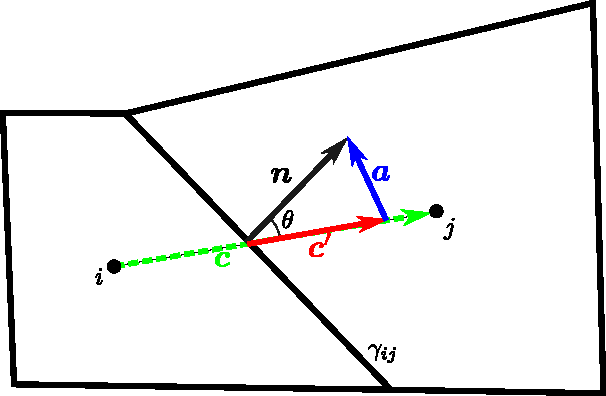
\includegraphics[width=0.4\linewidth]{skew_dfdn.pdf}
\caption{Ячейка периодичности в задаче обтекания бесконечной решётки}
\label{fig:skew_dfdn}
\end{figure}
Рассмотрим вычисление нормальной производной на грани $\gamma_{ij}$,
разделяющие точки коллокации $i$ и $j$ (\figref{fig:skew_dfdn}).
При использовании подхода с расширенным набором точек коллокации
не имеет значения, являются ли эти точки граничными коллокациями или внутренними.
Пусть вектор $\vec c$ соединяет точки коллокации.
За меру ортогональности примем значение угла $\theta$ 
между вектором единичной нормали $\vec n$ и вектором $\vec c$:
\begin{equation*}
\cos\theta = \frac{\vec n \cdot \vec c}{|\vec c|}.
\end{equation*}

Выделим некоторый вектор $\vec c'$, коллинеарный вектору $\vec c$.
И распишем вектор нормали как 
\begin{equation}
\label{eq:n_cprime_a}
\vec n = \vec c' + \vec a.
\end{equation}
Тогда
\begin{equation}
\label{eq:dudn_decomp}
\dfr{u}{n} = \nabla u \cdot \vec n = \nabla u \cdot \vec c' + \nabla u \cdot \vec a
= |\vec c'| \nabla u \cdot \frac{\vec c}{|\vec c|} + \nabla u \cdot \vec a.
\end{equation}
Первое слагаемое -- ортогональное приближение, которое 
с точностью до множителя $|\vec c'|$ равно ранее вычисленным
по разностным формулам \cref{eq:fvm_dudn_dudc,eq:fvm_bc1_approx}.
Второе -- поправка на скошенность.

Для реализации алгоритма с учётом этой поправки нужно решить следующие подзадачи:
\begin{itemize}
\item Задать длину $|\vec c'|$ (\secref{sec:cprime_a}),
\item Задать способ определения касательной производной $\nabla u\cdot \vec a$ (\secref{sec:fvm_duda}),
\item Собрать полученные соотношения в результирующую систему уравнений (\secref{sec:ortho_correction_assembly}).
\end{itemize}

\subsubsubsection{Методы разложения нормали}
\label{sec:cprime_a}
Рассмотрим различные варианты записи единичной нормали $\vec n$ в форме \cref{eq:n_cprime_a}.
Вектор $\vec c'$ сонаправлен заданному вектору $\vec c$, а вектор $\vec a$ может быть получен после определения $\vec c'$:
\begin{align*}
&\vec c' = |\vec c'| \frac{\vec c}{|\vec c|},\\
&\vec a = \vec n - \vec c'.
\end{align*}
То есть для конкретизации разложения  \cref{eq:n_cprime_a} нужно задать длину вектора $\vec c'$.
Рассмотрим три варианта её определения.

\paragraph{Поворот}

\begin{figure}[h!]
\centering
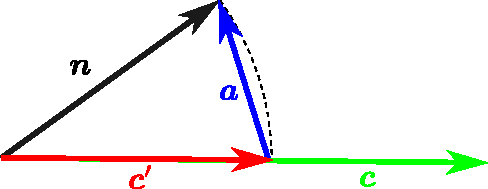
\includegraphics[width=0.4\linewidth]{cprime1.pdf}
\caption{Определение $\vec c'$ методом поворота}
\label{fig:cprime1}
\end{figure}

Положим $|\vec c'| = 1$. То есть положим длину искомого вектора равной длине единичной нормали $\vec n$ или повернём нормаль на угол $\theta$ (см. \figref{fig:cprime1}).
\begin{equation*}
\vec c' =  \frac{\vec c}{|\vec c|}.
\end{equation*}

\paragraph{Проекция}

\begin{figure}[h!]
\centering
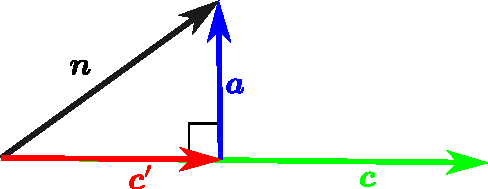
\includegraphics[width=0.4\linewidth]{cprime2.pdf}
\caption{Определение $\vec c'$ методом проекции}
\label{fig:cprime2}
\end{figure}

Определим вектор $\vec c'$ как проекцию вектора нормали на направление $\vec c$ (см. \figref{fig:cprime2}). Тогда
\begin{align*}
&|\vec c'| = \cos\theta = \frac{\vec n \cdot \vec c}{|\vec c|}, \\
&\vec c' = \frac{\vec n \cdot \vec c}{|\vec c|^2} \vec c
\end{align*}

В этом случае $|\vec c'| \leq 1$.
Таким образом, при записи нормальной производной \cref{eq:dudn_decomp} слагаемое с ортогональным приближением используется с коэффициентом, меньшим единицы.
Поэтому этот метод можно назвать методом нижней релаксации.

\paragraph{Обратная проекция}

\begin{figure}[h!]
\centering
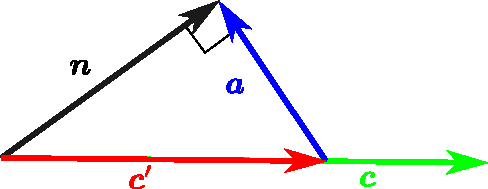
\includegraphics[width=0.4\linewidth]{cprime3.pdf}
\caption{Определение $\vec c'$ через обратную проекцию}
\label{fig:cprime3}
\end{figure}

Наоборот, опустим перпендикуляр с направления $\vec c$ на нормаль (см. \figref{fig:cprime3}):
\begin{align*}
&|\vec c'| = \frac{1}{\cos\theta} = \frac{|\vec c|}{\vec n \cdot \vec c}, \\
&\vec c' = \frac{\vec c}{\vec n \cdot \vec c}.
\end{align*}

Тогда, напротив $|\vec c'| \geq 1$, поэтому этот метод можно назвать методом верхней релаксации.
Отметим, что в этом случае вектор $\vec a$ будет параллелен грани $\gamma_{ij}$.

\subsubsubsection{Методы вычисления касательной производной}
\label{sec:fvm_duda}
Рассмотрим способы получить второе слагаемое из разложения \cref{eq:dudn_decomp}.
Напомним, что это разложение записывается для значения производной на грани конечноэлементной сетки:
\begin{equation*}
\left(\nabla u \cdot \vec a\right)_{\gamma_{ij}}
\end{equation*}
При этом функция $u$ задана своими значениями в точках коллокации, а вектор $\vec a$ известен (см. \secref{sec:cprime_a})

\paragraph{Определение через значение градиента в точках коллокации}
Пусть градиент $\nabla u$ также задан в точках коллокации.
Тогда значение на грани $\gamma_{ij}$ 
можно записать через линейную коминацию этих значений:
\begin{equation*}
\left(\nabla u\right)_{\gamma_{ij}} \approx w_i \left(\nabla u\right)_i + w_j \left(\nabla u\right)_j, \qquad w_i + w_j = 1.
\end{equation*}

Пусть $i$-ая точка коллокации граничная, тогда $w_i = 1, w_j = 0$.
Если же обе точки внутренние, то в простейшем случае можно взять $w_i = w_j = 0.5$.
В более сложных случаях можно подобрать весовые коэффициенты в зависимости от расстояние точки коллокации до грани.

Для определения градиента в точках коллокации применим алгорим опрелеления 
градинетов в центрах ячеек (см. \secref{sec:gradu_in_cells}).
К граничным точкам коллокации припишем значение градиента
из инцидентной с ней ячейкой.

Таким образом, пусть известны значение $(\nabla u)_i$ во внутренних точках коллокации. Тогда
значение градиента на границе будет равно
\begin{equation*}
\left(\nabla u\right)_{\gamma_{ij}} =
\begin{cases}
\frac12 \left(\nabla u\right)_i + \frac12 \left(\nabla u\right)_j, & \text{$i$ и $j$ -- внутренние точки коллокации}\\
\left(\nabla u\right)_i, & \text{$j$ -- граничная точка коллокации}\\
\left(\nabla u\right)_j & \text{$i$ -- граничная точка коллокации}.
\end{cases}
\end{equation*}

\paragraph{Прямая интерполяция}
TODO

\subsubsubsection{Учёт поправки при сборке СЛАУ}
\label{sec:ortho_correction_assembly}
Подставим в левую часть выражения \cref{eq:fvm_pois_int}
разложение для нормальной с учётом поправки на скошенность \cref{eq:dudn_decomp}
\begin{equation*}
-\arint{\left(|\vec c'| \dfr{u}{c} + \nabla u \cdot \vec a\right)}{\partial E_i}{\vec x} = \arint{f}{E_i}{\vec x}.
\end{equation*}
Первое слагаемое в левой части -- тоже самое слагаемое, которое
использовалось в ортогональном приближении. Оно вычисляется по формулам
\cref{eq:fvm_dudn_dudc,eq:fvm_bc1_approx}.
Второе слагаемое -- поправка на ортогональность, вычисляется по процедурам,
описанным в \secref{sec:fvm_duda}.

\paragraph{Явный учёт поправки}
Пусть нам известно некоторое приближение решения $\check u$.
Тогда мы можем вычислить скалярный сеточный вектор градиетов для каждой
грани конечнообъёмной сетки $\gamma_s$:
\begin{equation}
\label{eq:fvm_corr_vec}
{corr}_s = \left(\nabla \cdot \check u\right)_{s} \cdot \vec a_s
\end{equation}
Используем это решение для вычисление поправки на скошеннсть и
перенесём её вправо. Получим

\begin{equation*}
-\arint{|\vec c'| \dfr{u}{c}}{\partial E_i}{\vec x} = \arint{f}{E_i}{\vec x}+
\sum_{s\in{\rm S_i}} corr_s |\gamma_s|.
\end{equation*}
Здесь $\rm S_i$ -- индексы граней, инцидентных ячейке $i$.

При сборке матрицы левой части нужно внести изменения 
в процедуру \cref{eq:fvm_assem_bc_extended}, которая учтёт множитель $|\vec c'|$:
\begin{equation}
\label{eq:fvm_assem_extended_explicit_corr_lhs}
\begin{array}{ll}
\textbf{for } s \in\overline{0, N_f - 1}            & \textrm{-- цикл по всем граням}\\
\qquad i,j = \textrm{nei\_colloc(s)}                & \textrm{-- инцидентные точки коллокаций}\\
\qquad c = |\vec c'|_s                              & \textrm{-- поправка}\\
\qquad v = c \sfrac{|\gamma_{ij}|}{h_{ij}}          & \\
\qquad A_{ii} \pluseq  v, \quad A_{ij} \minuseq v   & \textrm{-- $i$-ая строка}\\ 
\qquad A_{jj} \pluseq  v, \quad A_{ji} \minuseq v   & \textrm{-- $j$-ая строка}\\ 
\textbf{endfor}                                     & \\
\end{array}
\end{equation}

Слагаемое в правой части будет учитано в аналогичной процедуре:
\begin{equation}
\label{eq:fvm_assem_extended_explicit_corr_rhs}
\begin{array}{ll}
\textbf{for } s \in\overline{0, N_f - 1}            & \textrm{-- цикл по всем граням}\\
\qquad i,j = \textrm{nei\_colloc(s)}                & \textrm{-- инцидентные точки коллокаций}\\
\qquad v = \textrm{corr}_s |\gamma_{ij}|            & \\
\qquad b_i \pluseq v                                & \\
\qquad b_j \pluseq v                                & \\
\textbf{endfor}                                     & \\
\end{array}
\end{equation}

Эта процедура так же правит значения 
для граничных точек коллокаций, поэтому дополнительная модификация
процедур для граничных условий второго и третьего рода не требуется.
Для периодических условий потребуется учесть суммирование строк после \cref{eq:fvm_assem_bcp_extended}
\begin{equation}
\label{eq:fvm_assem_bc_extended_explicit_corr_bcp}
\begin{array}{ll}
\textbf{for } s,s' \in\textrm{periodic\_pairs}           & \textrm{-- периодические пары граней}\\ 
\qquad i,j = \textrm{bnd\_col(s, s')}                    & \textrm{-- индексы граничных точек коллокации}\\
\qquad b_j \pluseq b_i                                   & \\
\qquad b_i = 0                                           & \\
\textbf{endfor}                                          & \\ 
\end{array}
\end{equation}

Тогда итоговый алгоритм сборки будет иметь следующий вид: \newline
{\rm Этап инициализации}
\begin{enumerate}
\item По алгоритмам \secref{sec:cprime_a} расчитать значения $|\vec c'|$  и $\vec a$ для каждой грани конечного объёма,
\item Собрать матрицу левой части по процедуре \cref{eq:fvm_assem_extended_explicit_corr_lhs}
\item Собрать вектор $b^0$ -- базовую часть правого столбца СЛАУ. Для этого инициализировать его нулями, потом применить алгоритм \cref{eq:fvm_assem_f}
\item Применить процедуры для граничных условий \cref{eq:fvm_assem_bc1_extended,eq:fvm_assem_bc2_extended,eq:fvm_assem_bc3_extended,eq:fvm_assem_bcp_extended}
\item Задать начальное приближение $\check u$
\end{enumerate}
{\rm Итерация на этапе расчёта}
\begin{enumerate}
\item По процедурам \secref{sec:fvm_duda} посчитать значение градиента $\nabla{\check u}$ для каждой грани конечнообъёмной сетки,
\item Найти вектор $corr$ по формуле \cref{eq:fvm_corr_vec}
\item Инициализировать вектор правой части $b = b^0$ и далее добавить в него поправку согласно \cref{eq:fvm_assem_extended_explicit_corr_rhs}
\item При наличии периодических условий применить процедуру \cref{eq:fvm_assem_bc_extended_explicit_corr_bcp}
\item Посчитать невязку $r = ||b - A \check u||$. Если она мала, выйти из цикла
\item Решить СЛАУ $A u = b$
\item Перейти на следующую итерацию $\check u = u$.
\end{enumerate}

\paragraph{Неявный учёт поправки}
TODO

\subsubsection{Вычисление градиентов в центрах ячеек}
\label{sec:gradu_in_cells}
\subsubsubsection{Метод Гаусса}
TODO
\subsubsubsection{Метод наименьших квадратов}
\label{sec:fvm_mse_grad}

Будем рассматривать узел $i$, имеющий $N_i$ соседних узлов $j$.
Для каждого $j$ можно записать линейное приближение
\begin{equation*}
u_j = u_i + |\vec c_{ij}| \dfr{u}{c_{ij}} = u_i + \vec c_{ij} \cdot \nabla u, \qquad j = \overline{0, N_i-1}.
\end{equation*}
Для двумерного случая можно записать:
\begin{equation*}
(\vec c_{ij})_x \, \dfr{u}{x} + (\vec c_{ij})_y \, \dfr{u}{y} = u_j - u_i, \qquad j = \overline{0, N_i - 1}.
\end{equation*}
Это выражение -- есть система линейных уравнений с двумя неизвестными $\dsfr{u}{x}$, $\dsfr{u}{y}$ 
и $N_i$ строками. Запишем её в матричном виде:
\begin{equation*}
\begin{array}{llll}
A y = f, &  \text{ где } & A_{j0} = (\vec c_{ij})_x & \quad A_{j1} = (\vec c_{ij})_y,\\
         &               & y_{0} = \dsfr{u}{x}      & \quad y_{1} = \dsfr{u}{y},\\
         &               & f_{j} = u_j - u_i &.
\end{array}
\end{equation*}
В двумерном случае размерность матрицы $A$ есть $[N_i, 2]$
(для трёхмерной задачи следуя аналогичным рассуждениям получим матрицу с размерностью $[N_i, 3]$).

При этом в двумерном случае у конечного элемента будет минимум три грани (или четыре в трёхмерном случае). То есть $N_i \geq 3$ 
и полученная система имеет неизвестных больше, чем количество уравнений.
Эта система в общем случае не имеет точного решения,
но можно найти такие $y$, при котором невязка будет минимальной.
Определим невязку как 
$$
r_i = \sum_{j=0}^{N_i}\left(A_{ij}y_j\right) - f_i, \qquad i=0, 1.
$$
и будем минимизировать её квадрат
$$
F = \sum_i r_i^2 \to \min
$$
Запишем условие экстремума как
$$
\dfr{F}{y_i} = 2 \sum_j r_j \dfr{r_j}{y_i} =
               2 \sum_j \left( \sum_k \left( A_{jk} y_k\right) - f_j \right)A_{ji} = 0, \qquad i=0,1.
$$
Отсюда получим систему уравнений
$$
\sum_j \left( A_{ji} \sum_k \left( A_{jk} y_k\right) \right) = \sum_j A_{ji}f_j = 0, \qquad i=0,1.
$$
Или, возвращаясь к матричной записи,
$$
A^{T} A y = A^{T}f.
$$
Полученная система имеет размерность $2\times2$ (или $3\times3$ в трёхмерном случае).
Значение компонент градиента в точке коллокации запишется как её прямое решение:
$$
y = \left(A^T A\right)^{-1} A^T f.
$$
Отметим, что матрица $A$ зависит только от геометрии сетки.
Поэтому в программной реализации матричное выражение $\left(A^T A\right)^{-1} A^T $ может быть расчитано 
один раз для каждого узла коллокации на этапе инициализации.
Тогда определение градиента в центрах ячеек на этапе решения задачи 
сведётся к сборке вектора $f$ и умножении его на это выражение.

\subsubsection{Неоднородный коэффициент диффузии}
\label{sec:fvm_nonconst_lambda}
Рассмотрим задачу в постановке \cref{eq:poissonnd_lam}.
Применение конечнообъёмных проеобразований по аналогии с 
\secref{sec:fvm_appr} даст следующие уравнения для конечного объёма $|E_i|$:
\begin{equation}
\label{eq:fvm_lambda_ij_scheme}
-\sum_j \lambda_{ij} \left(\dfr{u}{n}\right)_{ij} |\gamma_{ij}| = |E_i| f_i
\end{equation}
Здесь $\lambda_{ij}$ -- значение коэффициента диффузии
на грани между точками коллокации $i$ и $j$.
При этом в конечнообъёмной схеме все неизвестные скалярные поля, в том числе коэффициент диффузии, заданы только
в точках коллокаций. То есть задача состоит в том, чтобы зная $\lambda_i$, $\lambda_j$ выразить $\lambda_{ij}$.

Простейшим выходом будет использовать среднее арифметическое:
\begin{equation}
\label{eq:fvm_lambda_ij_0}
\lambda_{ij} = \frac{\lambda_{i} + \lambda_{j}}{2}
\end{equation}
Однако, это выражение не сохраняет порядок аппроксимации схемы.
Для записи более точного выражения, запишем выражение потоков слева и справа от грани $\gamma_{ij}$.
Для этого введём значение $u_{ij}$ на грани. В ортогональном приближении получим:
\begin{align*}
&\lambda_i \left( \dfr{u}{n} \right)_i \approx \lambda_{i}\frac{u_{ij} - u_i}{h_{ij}^-} , \\
&\lambda_j \left( \dfr{u}{n} \right)_j \approx \lambda_{j}\frac{u_{j} - u_{ij}}{h_{ij}^+}.
\end{align*}
Здесь $h_{ij}^+, h_{ij}^-$ -- доли расстояния $h_{ij}$, находящиеся в $i$-ой и $j$-ой ячейках, такие что 
$$h_{ij}^+ + h_{ij}^- = h_{ij}.$$
Эти выражения равны друг другу и равны суммарному потоку, вычисляемому через $\lambda_{ij}$:
\begin{equation}
\label{eq:fvm_dudn_lambda}
\lambda_{ij} \left(\dfr{u}{n}\right)_{ij} = \lambda_{ij} \frac{u_j - u_i}{h_{ij}}.
\end{equation}
Таким образом, мы получили систему из двух линейных уравнений
относительно неизвестных $\lambda_{ij}, u_{ij}$.
Выразим из это системы искомый коэффициент диффузии как среднее взвешенное гармоническое выражение
\begin{equation}
\label{eq:fvm_lambda_ij_1}
\lambda_{ij} = \frac{(h^+_{ij} + h^-_{ij}) \lambda_i \lambda_j}{\lambda_i h^+_{ij} + \lambda_j h^-_{ij}}.
\end{equation}
которое в приближении $h^+_{ij} \approx h^-_{ij}$ может быть упрощено до обычного среднегармонического
\begin{equation}
\label{eq:fvm_lambda_ij_2}
\lambda_{ij} = \frac{2\lambda_i\lambda_j}{\lambda_i + \lambda_j}.
\end{equation}

Нетрудно показать, что вычисление нормальной производной с учётом поправки на ортогональность
сохраняет эти выражения. Распишем поток слева и в центре с поправкой:
\begin{align*}
&\lambda_i \left( \dfr{u}{n} \right)_i = \lambda_{i}\left(\frac{u_{ij} - u_i}{h_{ij}^-} + \left(\nabla u\right)_i \cdot \vec a\right), \\
&\lambda_{ij} \left(\dfr{u}{n}\right)_{ij} = \lambda_{ij} \left(\frac{u_j - u_i}{h_{ij}} + \left(\nabla u\right)_{ij} \cdot \vec a\right).
\end{align*}
Если вычислять градиент на грани
как среднее взвешенное арифметическое:
\begin{equation*}
\left(\nabla u\right)_{ij} = \frac{h^-_{ij} \left(\nabla u\right)_i + h^+_{ij} \left(\nabla u\right)_j}{h^+_{ij} + h^-_{ij}}
\end{equation*}
то формула \cref{eq:fvm_lambda_ij_1} выполнится точно.

\subsubsection{Аппроксимация нормальной производной с учётом логарифмической особенности}
\label{sec:fvm_log_singularity}
Рассмотрим уравнение Лапласа ($f=0$) в двусвязной области, образованной
внешним контуром и внутренним кругом с центром в точке $\vec C$ (\figref{fig:radial_singularity}).
Будем считать, что значение искомой функции на внутренней границе постоянно.
\begin{figure}[h!]
\centering
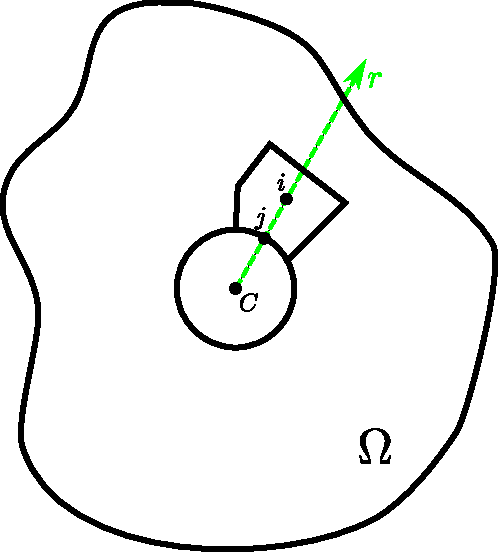
\includegraphics[width=0.4\linewidth]{radial_singularity.pdf}
\caption{Двусвязная область решения}
\label{fig:radial_singularity}
\end{figure}

Возьмём приграничную ячейку $i$ и граничную точку коллокации $j$.
Пусть точки $\vec C$, $\vec c_i$, $\vec c_j$ лежат на одной прямой. Координату
вдоль этой прямой будем называть $r$.
Будем считать, что граничное значение на внутреннем круге
сильно отличается (в большую или меньшую сторону) от
характерного значения $u$ в области расчёта.
Тогда в некотором приближении
решении в окрестности внутреннего круга можно
считать радиально симметричным: зависящим
только от $r$, но не от угла поворота радиус-вектора $\vec r$.
В приближении постоянного коэффициента диффузии такое решение будет удовлетворять уравнению 
\begin{equation*}
\frac 1r \dfr{}{r}\left( r \dfr{u}{r} \right) = 0.
\end{equation*}
Общим решением этого уравнение будет выражение
\begin{equation*}
u = A \ln r + B.
\end{equation*}
Коэффициенты $A$, $B$ выразим через значения
функции в точках коллокации:
\begin{equation*}
u(r_i) = u_i, \quad u(r_j) = u_j.
\end{equation*}
Тогда решение примет вид
\begin{equation*}
u(r) = \frac{\ln r - \ln r_i}{\ln r_j - \ln r_i}\left(u_j - u_i\right) + u_i.
\end{equation*}
Отсюда выразим нормальную производную на грани $\gamma_{ij}$:
\begin{equation} 
\label{eq:fvm_dudn_radial}
\left.\dfr{u}{n}\right|_{\gamma_{ij}} = -\left.\dfr{u}{r}\right|_{r=r_j} =  
\frac {1} {r_j} \, \frac{1}{\ln r_i - \ln r_j}\left(u_j - u_i\right).
\end{equation}
Это выражение будем использовать вместо
\cref{eq:fvm_dudn_dudc} для вычисления производной
на грани с логарифмической особенностью.

Учёт этой особенности можно реализовать за счёт модификации
коэффициента диффузии $\lambda_{ij}$ на граничной грани.
Выражение \cref{eq:fvm_dudn_radial}
можно свести к 
\cref{eq:fvm_dudn_lambda},
если считать диффузию в виде
\begin{equation}
\label{eq:fvm_ln_singularity_hij}
\lambda'_{ij} = \frac{\lambda_{ij}}{r_j} \frac{h_{ij}}{\ln r_i - \ln r_j}
\end{equation}

\subsubsection{Радиально-симметричная постановка}
\label{sec:fvm_radsym}
Теперь рассмотрим уравнение
\cref{eq:poissonnd_lam}
в цилиндрических координатах $(r, \theta, z)$ и радиально-симметричной постановке.
В частных производных определяющее уравнение запишется как
\begin{equation*}
\frac{1}{r}\dfr{}{r}\left( \lambda r \dfr{u}{r} \right) + \dfr{}{z}\left(\lambda \dfr{u}{z}\right) = f, \quad \dfr{u}{\theta} = 0.
\end{equation*}
Заметим, что общий вывод конечнообъёмной схемы
\cref{eq:fvm_lambda_ij_scheme}
использует только формулу Гаусса--Остроградского
\cref{eq:partint_div} в операторном виде.
Поэтому она будет справедлива в любой системе координат.

Особенность выбора радиально-симметричной постановки
проявится только в вычислении площади грани $|\gamma|$
и объёма ячейки $|E|$, которые в этой постановке являются телами
вращения вокруг оси $Oz$.
Вычислим объём как
\begin{equation*}
|E| = \int\limits_{E} d\vec x = \int\limits_0^{2\pi}\left(\iint\limits_{|E|_{rz}} r d r d z\right) d\phi  =
    2\pi \underbrace{\frac{1}{|E|_{rz}}\iint r \, d r d z}_{r_E} \, |E|_{rz} 
\end{equation*}
где $|E|_{rz}$ и $r_E$ -- объём и $r$--координата центра масс ячейки
в декартовой двумерной системе координат $(r, z)$.
Аналогичные рассуждения справедливы и для определения площади грани
через её двумерную площадь $|\gamma|_{rz}$ и центр масс $r_\gamma$.
Тогда окончательно запишем
\begin{equation}
\label{eq:fvm_radsym_measures}
\left|E\right| = 2 \pi r_E |E|_{rz}, \qquad
\left|\gamma\right| = 2 \pi r_\gamma |\gamma|_{rz}
\end{equation}



\appendix
\section{Задания для самостоятельной работы}
\subsection{Лекция 2 (20.09.25) МКО для решения уравнения Пуассона}
\label{sec:hw_fvm2d}
Теория: \secref{sec:FVM}

В тесте \cvar{poisson1-fvm} из файла \ename{poisson_fvm_test.cpp}
реализовано решение одномерного уравнения Пуассона с граничными условиями первого рода.
Проводится расчёт на сгущающихся сетках с количеством ячеек от 10 до 1000
и расчитываются среднеквадратичные нормы отклонения полученного численного решения от точного.
Решения сохраняются в vtk-файлы \ename{poisson1_fvm_n={}.vtk}.
Отталкиваясь от этой реализации необходимо:
\begin{enumerate}
\item написать аналогичный тест для двумерного уравнения,
\item провести серию расчётов на сгущающихся сетках разных типов (структурированных, pebi и скошенных),
\item визуализировать в Paraview полученное на этих сетках решение,
\item построить графики сеточной сходимости решения и определить порядок аппроксимации метода,
\item в тестовой программе производится сборка в цикле по ячейкам (\secref{sec:poisson_fvm_cellbased}).
      Следует переписать процедуру сборки в циклах по граням (\secref{sec:poisson_fvm_facebased}) и убедиться
      в идентичности результатов.
\end{enumerate}

\paragraph{Работа с сетками}
Все сетки в программе наследуются от абстрактного класса \cvar{IGrid}.
Необходимые для работы с сетками таблицы узлов, свойств и связности доступны
как виртуальные методы этого класса и объявлены в заголовочном файле \cvar{grid/i_grid.hpp}. Например
\begin{itemize}
\item \cvar{Point IGrid::point(size_t ipoint)} -- получить координату $i$-ой точки,
\item \cvar{double IGrid::face_area(size_t iface)} -- площадь $i$-ой грани,
\item \cvar{std::vector<int> IGrid::tab_cell_face(size_t icell)} -- получить список индексов граней для $i$-ой ячейки.
\end{itemize}
Грани (внутренние и граничные) пронумерованы сквозным образом.
Координаты точек всегда трёхмерные. Для двумерных и одномерных задач ``лишние'' координаты приравниваются нулю.

С помощью метода \cvar{IGrid::save_vtk} сетка может быть экспортирована в vtk формат и просмотрена в Paraview.
В \secref{sec:paraview} приведены некоторые приёмы визуализации численного решения.

Для построения двумерных сеток необходимо использовать класс \cvar{Grid2}:
\begin{cppcode}
// сетка 10х10 в единичном квадрате
auto grid = std::make_shared<RegularGrid2D>(0, 0, 1, 1, 10, 10);
\end{cppcode}

Неструктурированные сетки должны быть прочитаны из файла:

\begin{cppcode}
// Читаем сетку из файла /app/test_data/pebigrid.vtk
std::string fn = test_directory_file("pebigrid.vtk");
UnstructuredGrid2D grid = UnstructuredGrid2D::vtk_read(fn);
\end{cppcode}

Строить неструктурированные сетки следует с помощью утилиты \ename{hybmesh}.
В папке \ename{test_data} корневой директории репозитория лежат скрипты построения сеток:
\begin{itemize}
\item \ename{pebigrid.py} -- pebi--сетка,
\item \ename{tetragrid.py} -- сетка, состоящая из произвольных (скошенных) трех- и четырехугольников.
\end{itemize}
Инструкции по запуску этих скриптов смотри п. \ref{sec:hybmesh}.
Эти скрипты строят равномерную неструктурированную сетку
в единичном квадрате
и записывают её в файл vtk, который впоследствии можно загрузить
в расчётную программу.
В каждом из скриптов есть параметр \cvar{N}, означающий
примерное количество ячеек в итоговой сетке.
Меняя его значение можно строить сетки разного разрешения.

Для загрузки построенной сетки в решатель необходимо файл
с сеткой поместить в каталог \ename{test_data}
и далее загрузить её в класс \cvar{UnstructuredGrid2D}.

\paragraph{Тестовая задача}
Для тестирования двумерной задачи следует использовать двумерное точное решение.
Например,
\begin{cppcode}
double exact_solution(Point p) const override{
    double x = p.x;
    double y = p.y;
    return cos(10*x*x)*sin(10*y) + sin(10*x*x)*cos(10*x);
}
\end{cppcode}
Для вычисления правой части (функции \cvar{exact_rhs})
нужно подставить точное решение в исходное уравнение \cref{eq:poissonnd}.

\paragraph{График сходимости}
График сеточной сходимости следует строить по аналогии с графиком на \figref{fig:poisson_convergence}.
в логарифмических осях, где по оси абсцисс отлежено разбиение, а по оси ординат -- норма.
Разбиение -- это характерный линейный размер области расчёта, делённый на характерный линейный размер ячейки.
Для получения корректного порядка аппроксимации в двух- и трёхмерных задачах следует внимательно отнестись к вычислению этого параметра.
Для двумерной/трёхмерной области характерный размер можно определить как квадратный/кубический корень от объёма.

\paragraph{Рекомендации к программированию}
Свои программы следует оформлять в виде отдельных тестов (вместо того, чтобы модифицировать существующие).
Желательно, после того как программа заработает, сразу оставить несколько базовых \cvar{CHECK} проверок и
сделать локальный коммит, чтобы впоследствии легко распознавать и исправлять внесённые в дальнейшей работе ошибки.
К тому же наличие готовых тестов значительно облегчает рефакторинг кода.

При написании новых тестов следует переиспользовать уже написанный код, избегая копирования.
Для этого необходимо оформлять повторяющийся код в виде отдельных процедур и пользоваться механизмами наследования классов.

\section{Формулы и обозначения}
\subsection{Векторы}

\subsubsection{Обозначение}

Геометрические вектора обозначаются жирным шрифтом $\vec v$.
Скалярные координаты вектора -- через нижний индекс с обозначением
оси координат: $\left(v_x, v_y, v_z\right)$.
Если вектор $\vec u$ -- вектор скорости, то его декартовые координаты
имеют специальное обозначение $\vec u = \left(u, v, w\right)$.
Единичные вектора, соответствующие осям координат, обозначаются 
знаком $\hat\cdot$: $\vec{\hat x}$, $\vec{\hat y}$, $\vec{\hat z}$.
Координатные векторы обозначаются по символу первой оси. Например, $\vec x = (x, y, z)$ или $\vec \xi = (\xi, \eta, \zeta)$.

Операции в векторами имеют следующее обозначение (расписывая в декартовых координатах):
\begin{itemize}
\item
Умножение на скалярную функцию
\begin{equation}
\label{eq:vec_scalar}
f \vec u = (f u_x)\vec{\hat x} + (f u_y)\vec{\hat y} + (f u_z)\vec{\hat z};
\end{equation}
\item
Скалярное произведение
\begin{equation}
\label{eq:vec_dot}
\vec u \cdot \vec v = u_x v_x + u_y v_y + u_z v_z;
\end{equation}
\item
Векторное произведение
\begin{equation}
\label{eq:vec_cross}
\vec u\times\vec v = 
\left|
\begin{array}{ccc}
\vec{\hat x} & \vec{\hat y} & \vec{\hat z} \\
u_x & u_y & u_z \\
v_x & v_y & v_z
\end{array}
\right| = 
\left(u_y v_z - u_z v_y\right)\vec{\hat x} -
\left(u_x v_z - u_z v_x\right)\vec{\hat y} +
\left(u_x v_y - u_y v_x\right)\vec{\hat z}.
\end{equation}

\end{itemize}

В двумерном случае можно считать, что $u_z = v_z = 0$.
Тогда результатом векторного произведения согласно \cref{eq:vec_cross} 
будет вектор, направленный перпендикулярно плоскости $xy$:
$$
\vec u \times \vec v = (u_x v_y - u_y v_x)\vec{\hat z}.
$$
При работе с двумерными задачами, где ось $\vec z$ отсутствует,
обычно результатом векторного произведения считают скаляр
\begin{equation}
\label{eq:vec_cross_2d}
2D: \; \vec u \times \vec v = u_x v_y - u_y v_x.
\end{equation}
Геометрический смысл этого скаляра: площадь
параллелограмма, построенного на векторах $\vec u$ и $\vec v$.


\subsubsection{Набла--нотация}

Символ $\nabla$ -- есть псевдовектор, который выражает
покоординатные производные.
Для декартовой системы координат $(x, y, z)$ он запишется в виде
$$
\nabla = \left( \dfr{}{x}, \; \dfr{}{y}, \; \dfr{}{z} \right).
$$
В радиальной $(r, \phi, z)$:
$$
\nabla = \left( \dfr{}{r}, \; \frac{1}{r}\dfr{}{\phi}, \; \dfr{}{z} \right).
$$
В цилиндрической $(r, \theta, \phi)$:
$$
\nabla = \left( \dfr{}{r}, \; \frac{1}{r}\dfr{}{\theta}, \; \frac{1}{r\sin\theta}\dfr{}{\phi} \right).
$$
Удобство записи дифференциальных выражений с использованием $\nabla$ заключается в независимости записи от
вида системы координат.
Но если требуется обозначить производную по конкретной координате,
то, по аналогии с обычными векторами, это делается через нижний индекс:
$$
\nabla_n f = \dfr{f}{n}.
$$

Для этого символа справедливы все векторные операции, описанные ранее.
Так, применение $\nabla$ к скалярной функции аналогично умножению вектора
на скаляр \cref{eq:vec_scalar} (здесь и далее приводятся покоординатные выражения для декартовой системы):
\begin{equation}
\label{eq:del_grad}
\nabla f  = \left(\nabla_x f, \; \nabla_y f, \; \nabla_z f\right) = \dfr{f}{x}\vec{\hat x} + \dfr{f}{y}\vec{\hat y} + \dfr{f}{z}\vec{\hat z}.
\end{equation}
Результатом этой операции является вектор.

Скалярное умножение $\nabla$ на вектор $\vec v$ по аналогии с \cref{eq:vec_dot} -- есть дивергенция:
\begin{equation}
\label{eq:del_div}
\nabla \cdot \vec v  = \dfr{v_x}{x} + \dfr{v_y}{y} + \dfr{v_z}{z}
\end{equation}
результат которой -- скалярная функция.

Двойное применение $\nabla$ к скалярной функции -- это оператор Лапласа:
\begin{equation}
\label{eq:del_laplace}
\nabla \cdot \nabla f  = \nabla^2 f = \dfrq{f}{x} + \dfrq{f}{y} + \dfrq{f}{z}
\end{equation}

Ротор -- аналог векторного умножнения \cref{eq:vec_cross}:
\begin{equation}
\label{eq:del_rotor}
\nabla\times\vec v = 
\left|
\begin{array}{ccc}
\vec{\hat x} & \vec{\hat y} & \vec{\hat z} \\
\nabla_x & \nabla_y & \nabla_z \\
v_x & v_y & v_z
\end{array}
\right| = 
\left(\dfr{v_z}{y} - \dfr{v_y}{z}\right)\vec{\hat x} -
\left(\dfr{v_z}{x} - \dfr{v_x}{z}\right)\vec{\hat y} +
\left(\dfr{v_y}{x} - \dfr{v_x}{y}\right)\vec{\hat z}.
\end{equation}

\subsection{Интегрирование}
\label{sec:partint} 

\subsubsection{Формула Гаусса--Остроградского}

Формула Гаусса--Остроградского, связывающая
интегрирование по объёму $E$ с интегрированием по границе этого объёма $\Gamma$,
для векторного поля $\vec v$ имеет вид
\begin{equation}
\label{eq:partint_div}
\arint{\nabla\cdot\vec v}{E}{\vec x} = \arint{v_n}{\Gamma}{s},
\end{equation}
где $\vec n$ -- внешняя по отношению к области $E$ нормаль.
Смысл этой формулы можно проиллюстрировать на одномерном примере.
Пусть одномерное векторное поле $v_x = f(x)$ на отрезке $E = [a, b]$ задано
функцией, представленной на \figref{fig:div1d}.
\begin{figure}[h!]
\centering
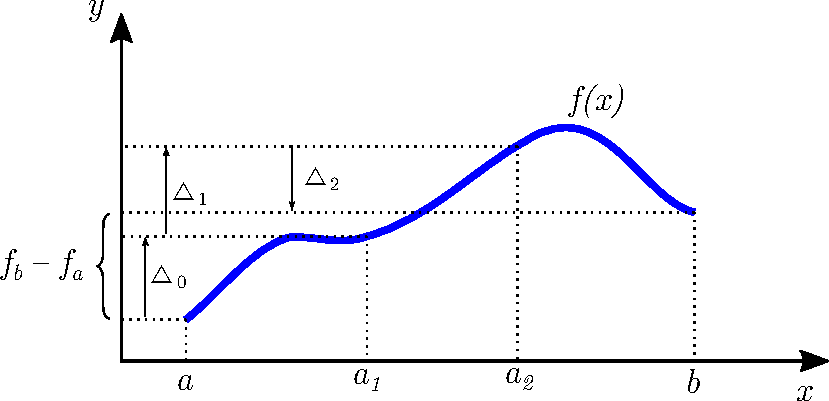
\includegraphics[width=0.6\linewidth]{div1d.pdf}
\caption{Формула Гаусса-Остроградского в одномерном случае}
\label{fig:div1d}
\end{figure}
Разобъем область на $N=3$ равномерных подобласти длины $h$. Тогда
расписывая интеграл как сумму, а производную через конечную разность, получим
$$
\arint{\dfr{f}{x}}{E}{x} \approx \sum_{i=0}^{2} h \left(\dfr{f}{x}\right)_{i+\tfrac12}
\approx\sum_{i=0}^{2}(f_{i+1} - f_{i})
= \triangle_0 + \triangle_1 + \triangle_2 = f_b - f_a.
$$
Очевидно что, при устремлении $N\to\infty$ правая часть предыдущего выражения не изменится.
То есть, сумма всех изменений функции в области есть изменение функции по её границам:
$$
\int\limits_{a}^{b}\dfr{f}{x}\,dx = f(b) - f(a).
$$
А формула \cref{eq:partint_div} -- есть многомерное обобщение этого выражения.

\subsubsection{Интегрирование по частям}

Подставив в \cref{eq:partint_div} $\vec v = f\vec u$, где $f$ -- некоторая скалярная функция, и 
расписав дивергенцию в виде
$$\nabla\cdot(f\vec u) = f\nabla\vec u + \vec u \cdot \nabla f$$
получим формулу интегрирования по частям
\begin{equation}
\label{eq:partint}
\arint{\vec u \cdot \nabla f}{E}{\vec x} = \arint{f u_n}{\Gamma}{s} - \arint{f\nabla\cdot \vec u}{E}{\vec x}
\end{equation}
Распишем некоторые частные случаи для формулы \cref{eq:partint}.
Для $\vec u = (n_x, 0, 0)$ получим
\begin{equation}
\label{eq:partint_ugrad_}
\arint{\dfr{f}{x}}{E}{\vec x} = \arint{f \cos(\vecangle{n}{x})}{\Gamma}{s}
\end{equation}
При $\vec u = \nabla g$
\begin{equation}
\label{eq:partint_laplace_fg}
\arint{f\left(\nabla^2 g \right)}{E}{\vec x} = \arint{f\dfr{g}{n}}{\Gamma}{s} - \arint{\nabla f \cdot \nabla g}{E}{\vec x}
\end{equation}
При $f=1$ и $\vec u = \nabla g$
\begin{equation}
\label{eq:partint_laplace}
\arint{\nabla^2 g}{E}{\vec x} = \arint{\dfr{g}{n}}{\Gamma}{s}
\end{equation}

\subsubsection{Численное интегрирование в заданной области}
Квадратурная формула
\begin{equation}
\label{eq:quadrature_formula}
\arint{f(\vec x)}{E}{\vec x} = \sum_{i=0}^{N-1} w_i f(\vec x_i)
\end{equation}
Она определяется заданием узлов интегрирования $\vec x_i$ 
и соответствующих весов $w_i$.

\subsection{Интерполяционные полиномы}

\subsubsection{Многочлен Лагранжа}

\subsubsubsection{Узловые базисные функции}

Рассмотрим функцию $f(\xi)$, заданную в области $D$.
Внутри этой области зададим $N$ узловых
точек $\xi_i, i=\overline{0,N-1}$.
Приближение функции $f$ будем искать в виде
\begin{equation}
\label{eq:nodal_basis}
f(\xi) \approx \sum_{i=0}^{N-1} f_i \phi_i(\xi),
\end{equation}
где  $f_i = f(\xi_i)$, $\phi_i$ -- узловая базисная функция.
Потребуем, чтобы это выражение выполнялось точно для всех
заданных узлов интерполяции $\xi = \xi_i$. Тогда, исходя из определения \cref{eq:nodal_basis}, запишем условие 
на узловую базисную функцию
\begin{equation}
\label{eq:nodal_bases_conditions}
\phi_i(\xi_j) = 
\begin{cases}
1, &\quad i = j, \\
0, &\quad i \neq j.
\end{cases}
\end{equation}
Дополнительно потребуем, чтобы формула \cref{eq:nodal_basis} была
точной для постоянных функций
$$
f(\xi)=\const \hence f_i = \const.
$$
Тогда для любого $\xi$ должно выполняться условие
\begin{equation}
\label{eq:nodal_bases_unitsum}
\sum_{i=0}^{N-1} \phi_i(\xi) = 1, \qquad \xi \in D.
\end{equation}

Задача построения интерполяционной функции состоит
в конкретном определении узловых базисов
$\phi_i(\xi)$ по заданному набору
узловых точек $\xi_i$ и значениям
функции в них $f_i$. Будем искать базисы
в виде многочленов вида
\begin{equation}
\label{eq:nodal_basis_1d_decomp}
\phi_i(\xi) = \sum_{a} A_i^{(a)} \xi^{a} =
A_i^{(0)} + 
A_i^{(1)} \xi + 
A_i^{(2)} \xi^2 +  \ldots, \qquad i = \overline{0, N-1}.
\end{equation}
Определять коэффициенты $A^{(a)}_i$ будем из условий \cref{eq:nodal_bases_conditions},
которое даёт $N$ линейных уравнений относительно неизвестных $A_i^{(a)}$ для каждого $i=\overline{0, N-1}$.
Таким образом, в выражениях \cref{eq:nodal_basis_1d_decomp} должно быть
ровно $N$ слагаемых.
Будем использовать последовательный набор степеней: $a=\overline{0,N-1}$.
Выпишем систему линейных уравнений для $0$-ой базисной функции
\begin{equation*}
\begin{aligned}
& \phi_0(\xi_0) = A_0^{(0)} + A_0^{(1)} \xi_0 + A_0^{(2)} \xi_0^2 + A_0^{(3)} \xi_0^3 + \ldots = 1, \\
& \phi_0(\xi_1) = A_0^{(0)} + A_0^{(1)} \xi_1 + A_0^{(2)} \xi_1^2 + A_0^{(3)} \xi_1^3 + \ldots = 0, \\
& \phi_0(\xi_2) = A_0^{(0)} + A_0^{(1)} \xi_2 + A_0^{(2)} \xi_2^2 + A_0^{(3)} \xi_2^3 + \ldots = 0, \\
& \ldots
\end{aligned}
\end{equation*}
или в матричном виде
\begin{equation*}
\left(
\begin{array}{ccccc}
1 & \xi_0 & \xi_0^2 & \xi_0^3 & \ldots \\[5pt]
1 & \xi_1 & \xi_1^2 & \xi_1^3 & \ldots \\[5pt]
1 & \xi_2 & \xi_2^2 & \xi_2^3 & \ldots \\[5pt]
1 & \xi_3 & \xi_3^2 & \xi_3^3 & \ldots \\[5pt]
\ldots &&&&
\end{array}
\right)
\left(
\begin{array}{c}
A_0^{(0)} \\[5pt]
A_0^{(1)} \\[5pt]
A_0^{(2)} \\[5pt]
A_0^{(3)} \\[5pt]
\vdots
\end{array}
\right)
=
\left(
\begin{array}{c}
1 \\[5pt]
0 \\[5pt]
0 \\[5pt]
0 \\[5pt]
\vdots
\end{array}
\right)
\end{equation*}
Записывая аналогичные выражения для остальных базисных функций, получим систему матричных уравнений
вида $C A = E$:
\begin{equation*}
\left(
\begin{array}{ccccc}
1 & \xi_0 & \xi_0^2 & \xi_0^3 & \ldots \\[5pt]
1 & \xi_1 & \xi_1^2 & \xi_1^3 & \ldots \\[5pt]
1 & \xi_2 & \xi_2^2 & \xi_2^3 & \ldots \\[5pt]
1 & \xi_3 & \xi_3^2 & \xi_3^3 & \ldots \\[5pt]
\ldots &&&&
\end{array}
\right)
\left(
\begin{array}{ccccc}
A_0^{(0)} & A_1^{(0)} & A_2^{(0)} & A_3^{(0)} & \ldots\\[5pt]
A_0^{(1)} & A_1^{(1)} & A_2^{(1)} & A_3^{(1)} &       \\[5pt]
A_0^{(2)} & A_1^{(2)} & A_2^{(2)} & A_3^{(2)} &       \\[5pt]
A_0^{(3)} & A_1^{(3)} & A_2^{(3)} & A_3^{(3)} &       \\[5pt]
\vdots
\end{array}
\right)
=
\left(
\begin{array}{ccccc}
1 & 0 & 0 & 0 & \ldots \\[5pt]
0 & 1 & 0 & 0 &        \\[5pt]
0 & 0 & 1 & 0 &        \\[5pt]
0 & 0 & 0 & 1 &        \\[5pt]
\vdots
\end{array}
\right)
\end{equation*}
Отсюда матрица неизвестных коэффициентов $A$ определится как
\begin{equation}
\label{eq:nodal_basic_amat}
A = C^{-1} = 
\left(
\begin{array}{ccccc}
1 & \xi_0 & \xi_0^2 & \xi_0^3 & \ldots \\[5pt]
1 & \xi_1 & \xi_1^2 & \xi_1^3 & \ldots \\[5pt]
1 & \xi_2 & \xi_2^2 & \xi_2^3 & \ldots \\[5pt]
1 & \xi_3 & \xi_3^2 & \xi_3^3 & \ldots \\[5pt]
\ldots &&&&
\end{array}
\right) ^{-1}.
\end{equation}

Подставляя полином \cref{eq:nodal_basis_1d_decomp} в условие согласованности \cref{eq:nodal_bases_unitsum},
получим требование
\begin{equation*}
\sum_{i=0}^{N-1} A_i^{(a)} = 
\begin{cases}
1, \quad a=0, \\
0, \quad a=\overline{1,N-1}.
\end{cases}
\end{equation*} 
То есть сумма всех свободных членов в интерполяционных полиномах должна
быть равна единице, а сумма коэффициентов при остальных степенях -- нулю.
Можно показать, что это свойство выполняется для любой матрицы $A=C^{-1}$,
в случае, если первый столбец матрицы $C$ состоит из единиц.
То есть условие согласованности требует наличие свободного члена
с интерполяционном полиноме.


\subsubsubsection{Интерполяция в параметрическом отрезке}
\label{sec:segment_bases}
Будем рассматривать область интерполяции $D=[-1, 1]$.
В качестве первых двух узлов интерполяции возьмем границы области:
$\xi_0 = -1$, $\xi_1 = 1$.
\paragraph{Линейный базис}
Будем искать интерполяционный базис в виде
$$
\phi_i(\xi) = A_i^{(0)} + A_i^{(1)} \xi.
$$
на основе двух условий:
$$
\phi_i(-1) = A_i^{(0)} - A_i^{(1)} = \delta_{0i}, \quad \phi_i(1) = A_i^{(0)} + A_i^{(1)}\delta_{1i}.
$$
Составим матрицу $C$, записав эти условия в матричном виде
$$
C =
\left(
\begin{array}{l|rr}
      & A^{(0)} & A^{(1)}\\
\hline
\phi(-1) & 1 & -1 \\[5pt]
\phi(1) & 1 &  1 \\[5pt]
\end{array}
\right)
$$
и, согласно \cref{eq:nodal_basic_amat}, найдём матрицу коэффициентов
$$
A =
\left(
\begin{array}{cc}
A_0^{(0)} & A_1^{(0)} \\[5pt]
A_0^{(1)} & A_1^{(1)} \\[5pt]
\end{array}
\right) = C^{-1} =
\left(
\begin{array}{l|rr}
     & \phi_0   & \phi_1  \\
\hline
1    & \frac12  & \frac12 \\[5pt]
\xi  & -\frac12 & \frac12 \\[5pt]
\end{array}
\right).
$$
Отсюда узловые базисные функции примут вид (\figref{fig:basis1d_linear})
\begin{equation}
\label{eq:segment_linear_basis}
\begin{aligned}
&\phi_0(\xi) = \frac{1 - \xi}{2}, \\
&\phi_1(\xi) = \frac{1 + \xi}{2}.
\end{aligned}
\end{equation}
Окончательно интерполяционная функция из определения \cref{eq:nodal_basis}
примет вид
$$
f(\xi) \approx \frac{1 - \xi}{2} f(-1) + \frac{1 + \xi}{2} f(1).
$$
\begin{figure}[h!]
\centering
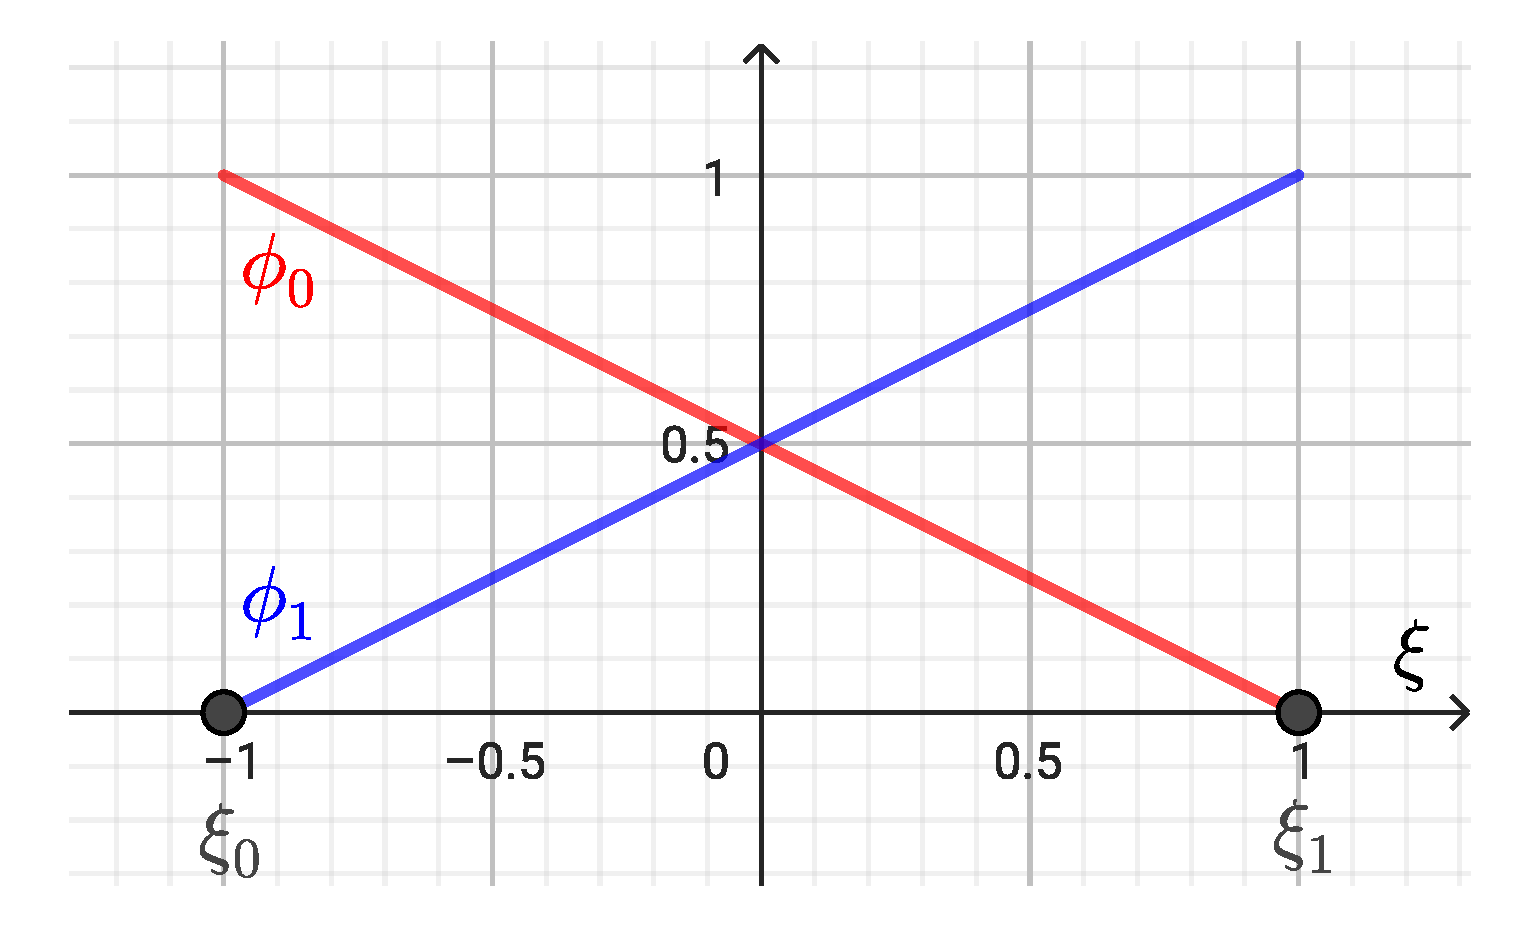
\includegraphics[width=0.4\linewidth]{basis1d_linear.pdf}
\caption{Линейный базис в параметрическом отрезке}
\label{fig:basis1d_linear}
\end{figure}

\paragraph{Квадратичный базис}
Будем искать интерполяционный базис в виде
$$
\phi_i(\xi) = A_i^{(0)} + A_i^{(1)} \xi + A_i^{(2)} \xi^2.
$$
По сравнению с линейным случаем, в форму базиса добавился ещё один неизвестый коэффициент $A_i^{(2)}$,
поэтому в набор условий \cref{eq:nodal_bases_conditions} требуется ещё одно уравнение (ещё одна узловая точка).
Поместим её в центр параметрического сегмента $\xi_2 = 0$. Далее будем действовать по
аналогии с линейным случаем:
$$
C = \left(
\begin{array}{l|rrr}
         &  A^{(0)} & A^{(1)}   & A^{(2)} \\ 
\hline
\phi(-1) & 1 & -1 & 1\\[5pt]
\phi(1)  & 1 &  1 & 1\\[5pt]
\phi(0)  & 1 &  0 & 0
\end{array}
\right)
\hence
A = C^{-1} = \left(
\begin{array}{l|rrr}
       & \phi_0   & \phi_1   & \phi_2 \\
\hline
 1     & 0        &  0       &  1     \\[5pt]
 \xi   & -\frac12 &  \frac12 &  0     \\[5pt]
 \xi^2 &  \frac12 &  \frac12 & -1     \\[5pt]
\end{array}
\right).
$$
Узловые базисные функции для квадратичной интерполяции примут вид (\figref{fig:basis1d_quadratic})
\begin{equation}
\label{eq:segment_quadratic_basis}
\begin{aligned}
&\phi_0(\xi) = \frac{\xi^2 - \xi}{2}, \\
&\phi_1(\xi) = \frac{\xi^2 + \xi}{2}, \\
&\phi_2(\xi) = 1 - \xi^2.
\end{aligned}
\end{equation}

\begin{figure}[h!]
\centering
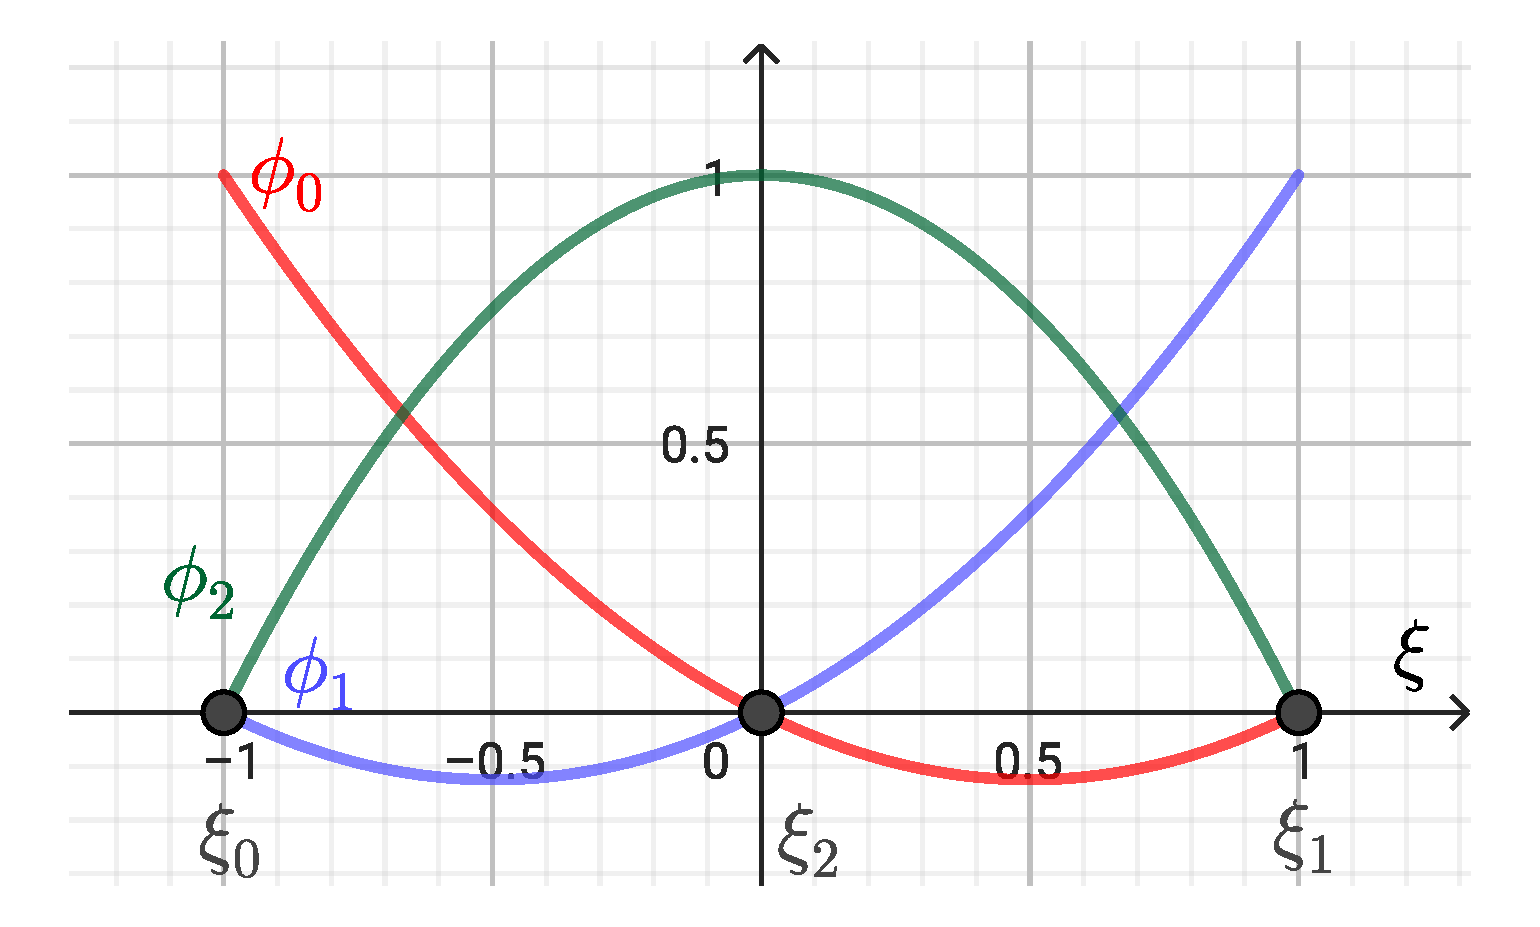
\includegraphics[width=0.4\linewidth]{basis1d_quadratic.pdf}
\caption{Квадратичный базис в параметрическом отрезке}
\label{fig:basis1d_quadratic}
\end{figure}

\paragraph{Кубический базис}
Интерполяционный базис будет иметь вид
$$
\phi_i(\xi) = A_i^{(0)} + A_i^{(1)} \xi + A_i^{(2)} \xi^2 + A_i^{(3)} \xi^3.
$$
Для нахождения четырёх коэффициентов нам понадобится четыре узла интерполяции.
Две из них -- это границы параметрического отрезка. Остальные две разместим
так, чтобы разбить отрезок на равные интервалы:
$\xi_2 = -\tfrac13$, $\xi_3 = \tfrac13$.
Далее вычислим матрицу коэффициентов:
$$
C =
\left(
\begin{array}{l|rrrr}
                &  A^{(0)}  &  A^{(1)}      & A^{(2)}     & A^{(3)}         \\
\hline
\phi(-1)        &  1  & -1        & 1         &  -1           \\[5pt]
\phi( 1)        &  1  & 1         & 1         &   1           \\[5pt]
\phi(-\tfrac13) &  1  & -\tfrac13 & \tfrac19  &  -\tfrac1{27} \\[5pt]
\phi(\tfrac13)  &  1  &  \tfrac13 & \tfrac19  &   \tfrac1{27}
\end{array}
\right)
\hence
A = C^{-1} =
\frac{1}{16}
\left(
\begin{array}{l|rrrr}
      & \phi_0 & \phi_1 & \phi_2 & \phi_3 \\
\hline
1     & -1     & -1     &   9    &  9     \\[5pt]
\xi   &  1     & -1     & -27    &  27    \\[5pt]
\xi^2 &  9     &  9     & -9     & -9     \\[5pt]
\xi^3 & -9     &  9     &  27    & -27   
\end{array}
\right)
$$
Узловые базисные функции для квадратичной интерполяции примут вид (\figref{fig:basis1d_cubic})
\begin{equation}
\label{eq:segment_cubic_basis}
\begin{aligned}
&\phi_0(\xi) = \frac{1}{16}\left(-1 + \xi + 9 \xi^2 -9 \xi^3\right), \\
&\phi_1(\xi) = \frac{1}{16}\left(-1 - \xi + 9 \xi^2 +9 \xi^3\right), \\
&\phi_2(\xi) = \frac{1}{16}\left(9 -27 \xi - 9\xi^2 + 27 \xi^3\right), \\
&\phi_3(\xi) = \frac{1}{16}\left(9 +27 \xi - 9\xi^2 - 27 \xi^3\right), \\
\end{aligned}
\end{equation}

\begin{figure}[h!]
\centering
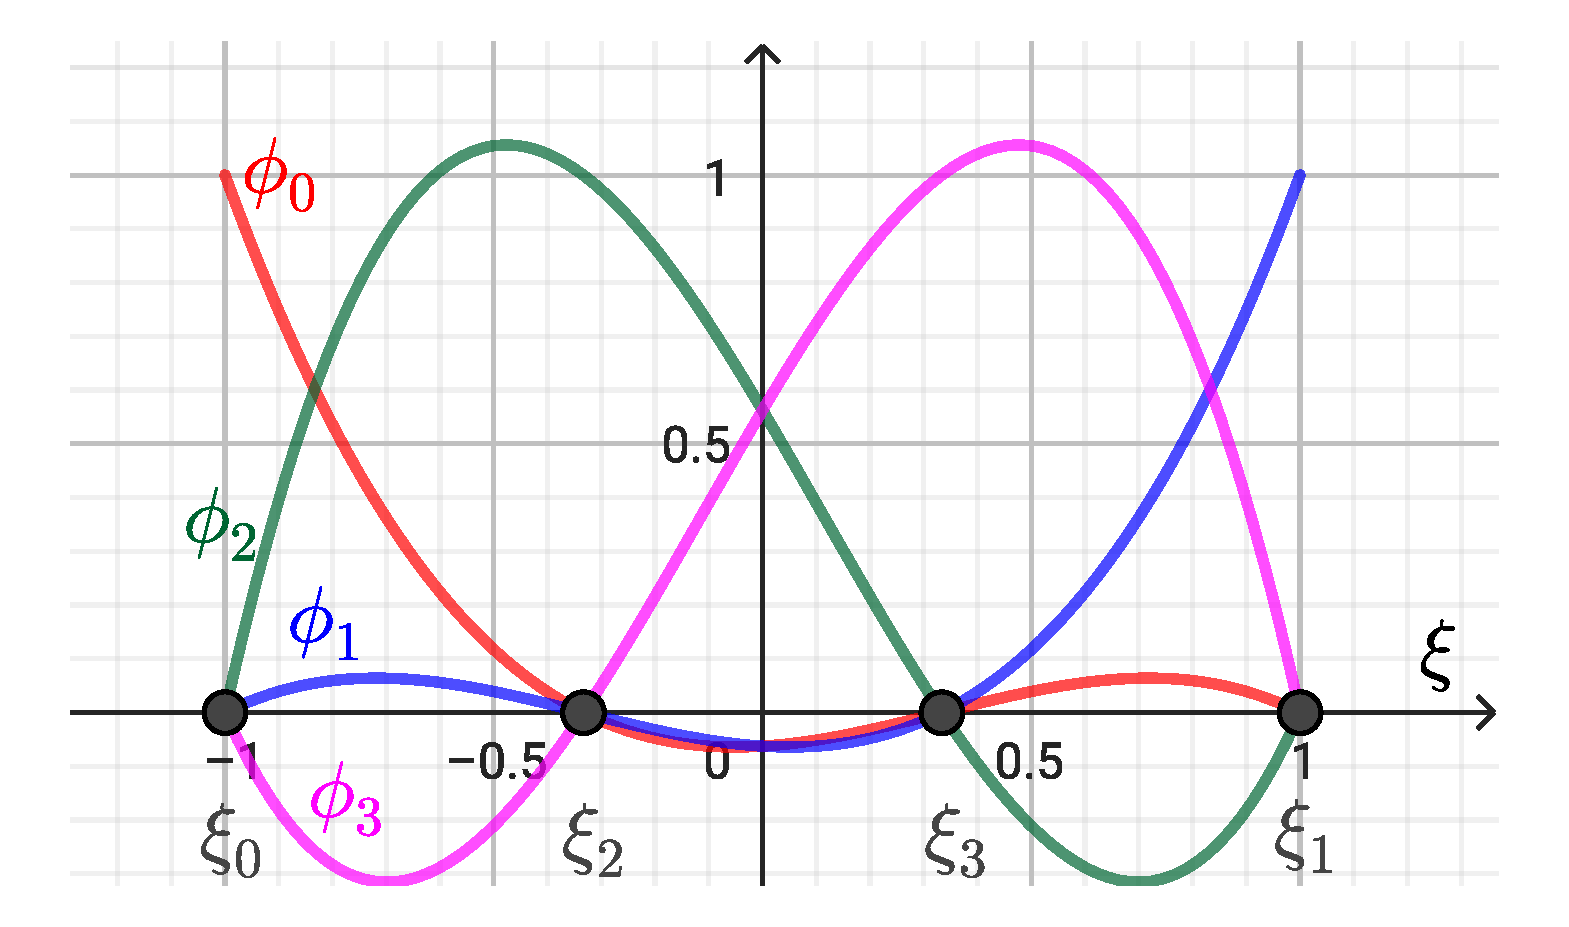
\includegraphics[width=0.4\linewidth]{basis1d_cubic.pdf}
\caption{Кубический базис в параметрическом отрезке}
\label{fig:basis1d_cubic}
\end{figure}

На \figref{fig:basis1d_compare} представлено сравнение результатов
аппроксимации функции $f(x) = -x + \sin(2 x + 1)$ линейным, квадратичным и кубическим базисом.
Видно, что все интерполяционные приближения точно попадают в функцию в своих
узлах интерполяции, а между узлами происходит аппроксимация полиномом соответствующей степени.

\begin{figure}[h!]
\centering
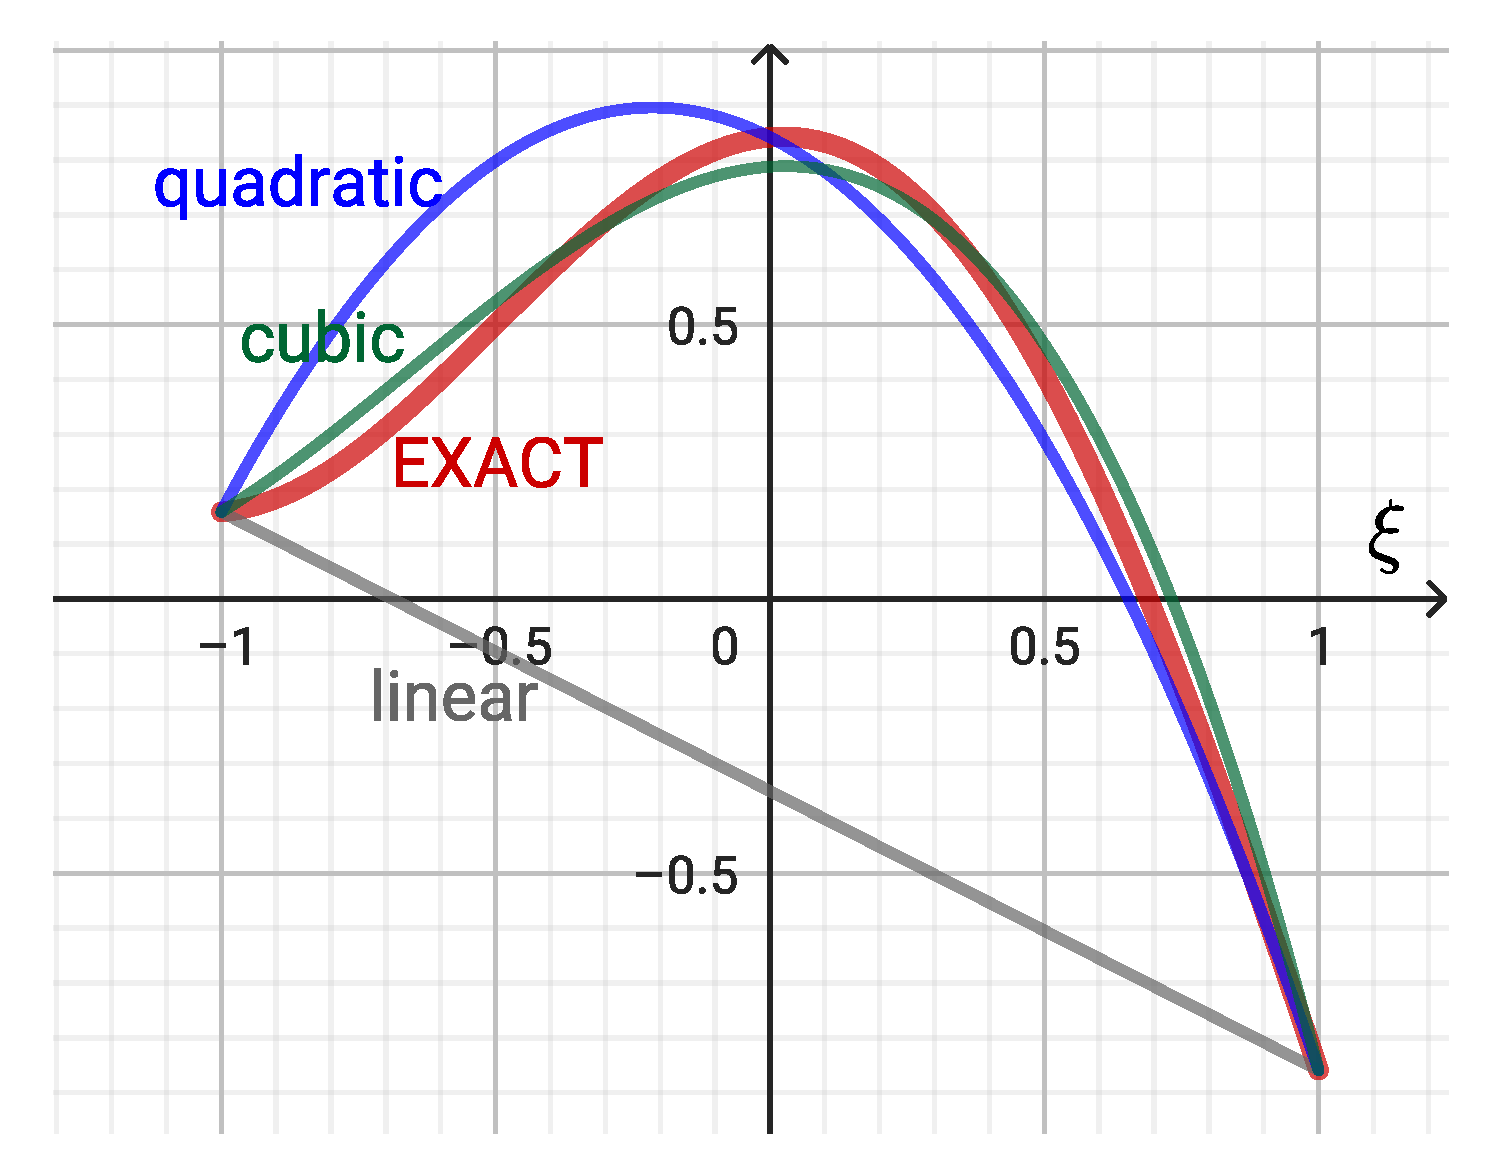
\includegraphics[width=0.4\linewidth]{basis1d_compare.pdf}
\caption{Результат интерполяции}
\label{fig:basis1d_compare}
\end{figure}

\subsubsubsection{Интерполяция в параметрическом треугольнике}
\label{sec:triangle_bases}
Теперь рассмотрим двумерное обобщение формулы
\begin{figure}[h!]
\centering
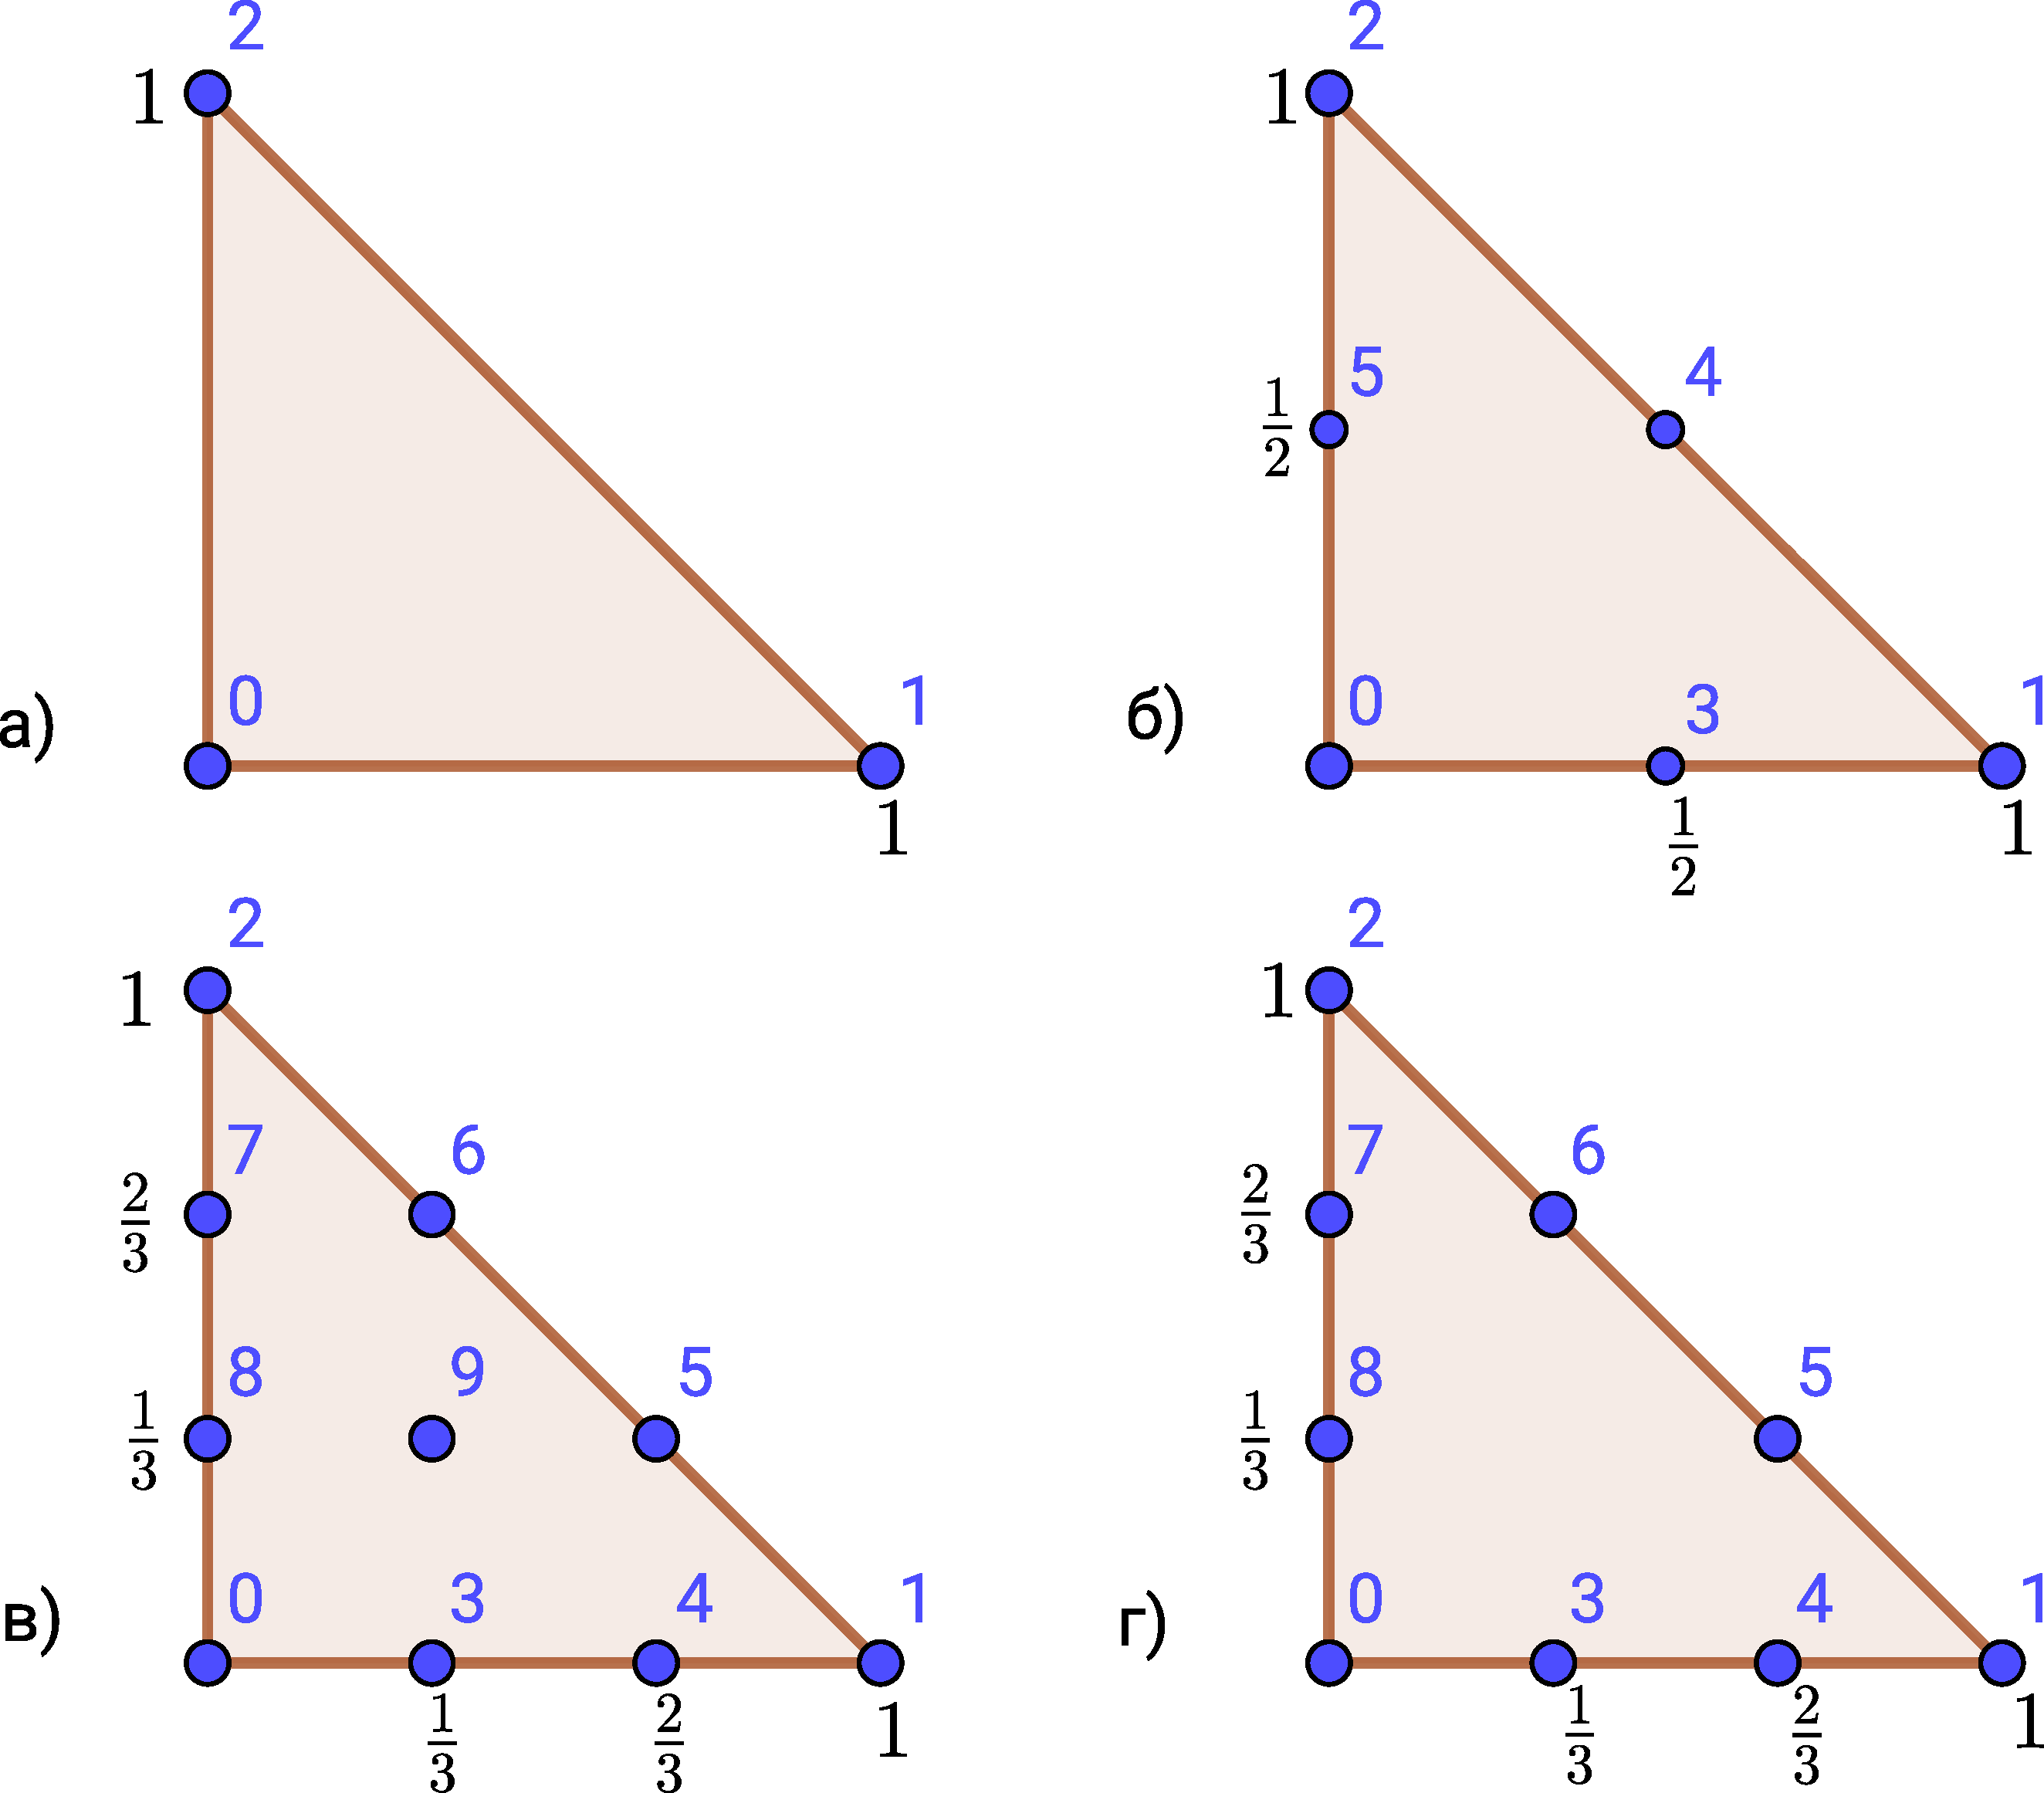
\includegraphics[width=0.5\linewidth]{triangle_basis_points.pdf}
\caption{Расположение узловых точек в параметрическом треугольнике. а) линейный базис, б) квадратичный базис, в) кубический базис, г) неполный кубический базис}
\label{fig:triangle_basis_points}
\end{figure}
\paragraph{Линейный базис}

\begin{equation*}
\phi_i(\xi, \eta) = A_i^{(00)} + A_i^{(10)} \xi + A_i^{(01)} \eta.
\end{equation*}
\begin{equation*}
C = \left(
\begin{array}{l|ccc}
                  & A^{(00)}   & A^{(10)} & A^{(01)} \\
\hline
\phi(0, 0) & 1   & 0   & 0    \\[5pt]
\phi(1, 0) & 1   & 1   & 0    \\[5pt]
\phi(0, 1) & 1   & 0   & 1
\end{array}
\right)
\hence
A = C^{-1} = 
\left(
\begin{array}{l|rrr}
     & \phi_0 & \phi_1 & \phi_2 \\
\hline
1    & 1      & 0      & 0      \\[5pt]
\xi  &-1      & 1      & 0      \\[5pt]
\eta &-1      & 0      & 1
\end{array}
\right)
\end{equation*}

\begin{equation}
\label{eq:triangle_linear_basis}
\begin{aligned}
&\phi_0(\xi, \eta) = 1 - \xi - \eta, \\
&\phi_1(\xi, \eta) = \xi, \\
&\phi_2(\xi, \eta) = \eta, \\
\end{aligned}
\end{equation}

\begin{figure}[h!]
\centering
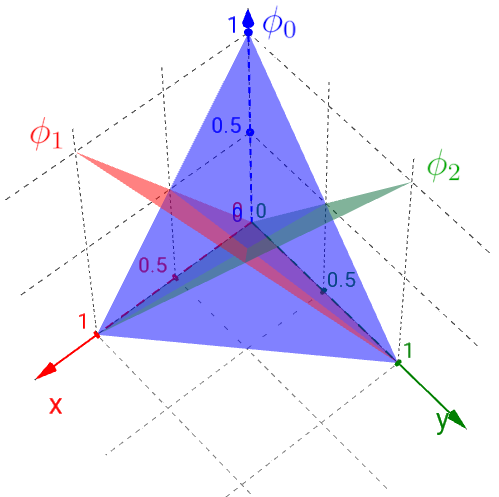
\includegraphics[width=0.4\linewidth]{basis2d_linear.png}
\caption{Линейный базис в параметрическом треугольнике}
\label{fig:basis2d_linear}
\end{figure}


\paragraph{Квадратичный базис}
\begin{equation*}
\phi_i(\xi, \eta) = A_i^{(00)} + A_i^{(10)} \xi + A_i^{(01)} \eta + A_i^{(11)} \xi \eta + A_i^{(20)} \xi^2 + A_i^{(02)} \eta^2.
\end{equation*}

\begin{equation*}
C =
\left(
\begin{array}{l|cccccc}
                     & A^{(00)} & A^{(10)}      & A^{(01)}  & A^{(11)}  & A^{(20)}    & A^{(02)}   \\[5pt]
\hline
\phi(0, 0)               & 1 &  0       &  0          &   0      &    0     &   0      \\[5pt]
\phi(1, 0)               & 1 &  1       &  0          &   0      &    1     &   0      \\[5pt]
\phi(0, 1)               & 1 &  0       &  1          &   0      &    0     &   1      \\[5pt]
\phi(\tfrac12, 0)        & 1 & \tfrac12 &  0          &   0      & \tfrac14 &   0      \\[5pt]
\phi(\tfrac12, \tfrac12) & 1 & \tfrac12 &  \tfrac12   & \tfrac14 & \tfrac14 & \tfrac14 \\[5pt]
\phi(0, \tfrac12)        & 1 &  0       &  \tfrac12   &   0      &    0     & \tfrac14 
\end{array}
\right)
\hence
A = \left(
\begin{array}{l|rrrrrr}
        & \phi_0 & \phi_1 & \phi_2 & \phi_3 & \phi_4 & \phi_5 \\[5pt]
\hline
1       & 1  &  0 & 0 & 0 & 0 & 0\\[5pt]
\xi     & -3 & -1 & 0 & 4 & 0 & 0\\[5pt]
\eta    & -3 & 0 & -1 & 0 & 0 & 4\\[5pt]
\xi\eta & 4 & 0 & 0 & -4 & 4 & -4\\[5pt]
\xi^2   & 2 & 2 & 0 & -4 & 0 & 0 \\[5pt]
\eta^2  & 2 & 0 & 2 & 0 & 0 & -4
\end{array}
\right)
\end{equation*}

\begin{figure}[h!]
\centering
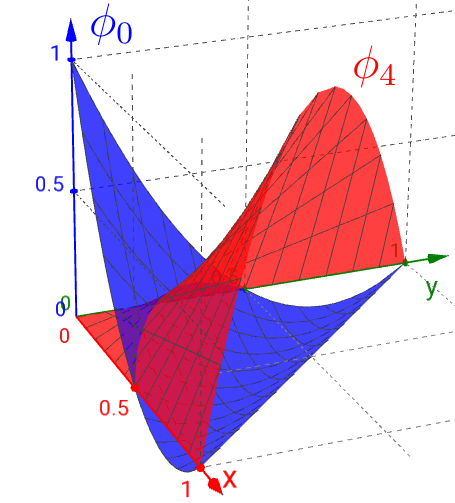
\includegraphics[width=0.3\linewidth]{basis2d_quadratic.png}
\caption{Квадратичные функции $\phi_0$, $\phi_4$ в параметрическом треугольнике}
\label{fig:basis2d_quadratic}
\end{figure}

\paragraph{Кубический базис}
TODO

\paragraph{Неполный кубический базис}
TODO

\subsubsubsection{Интерполяция в параметрическом квадрате}
\begin{figure}[h!]
\centering
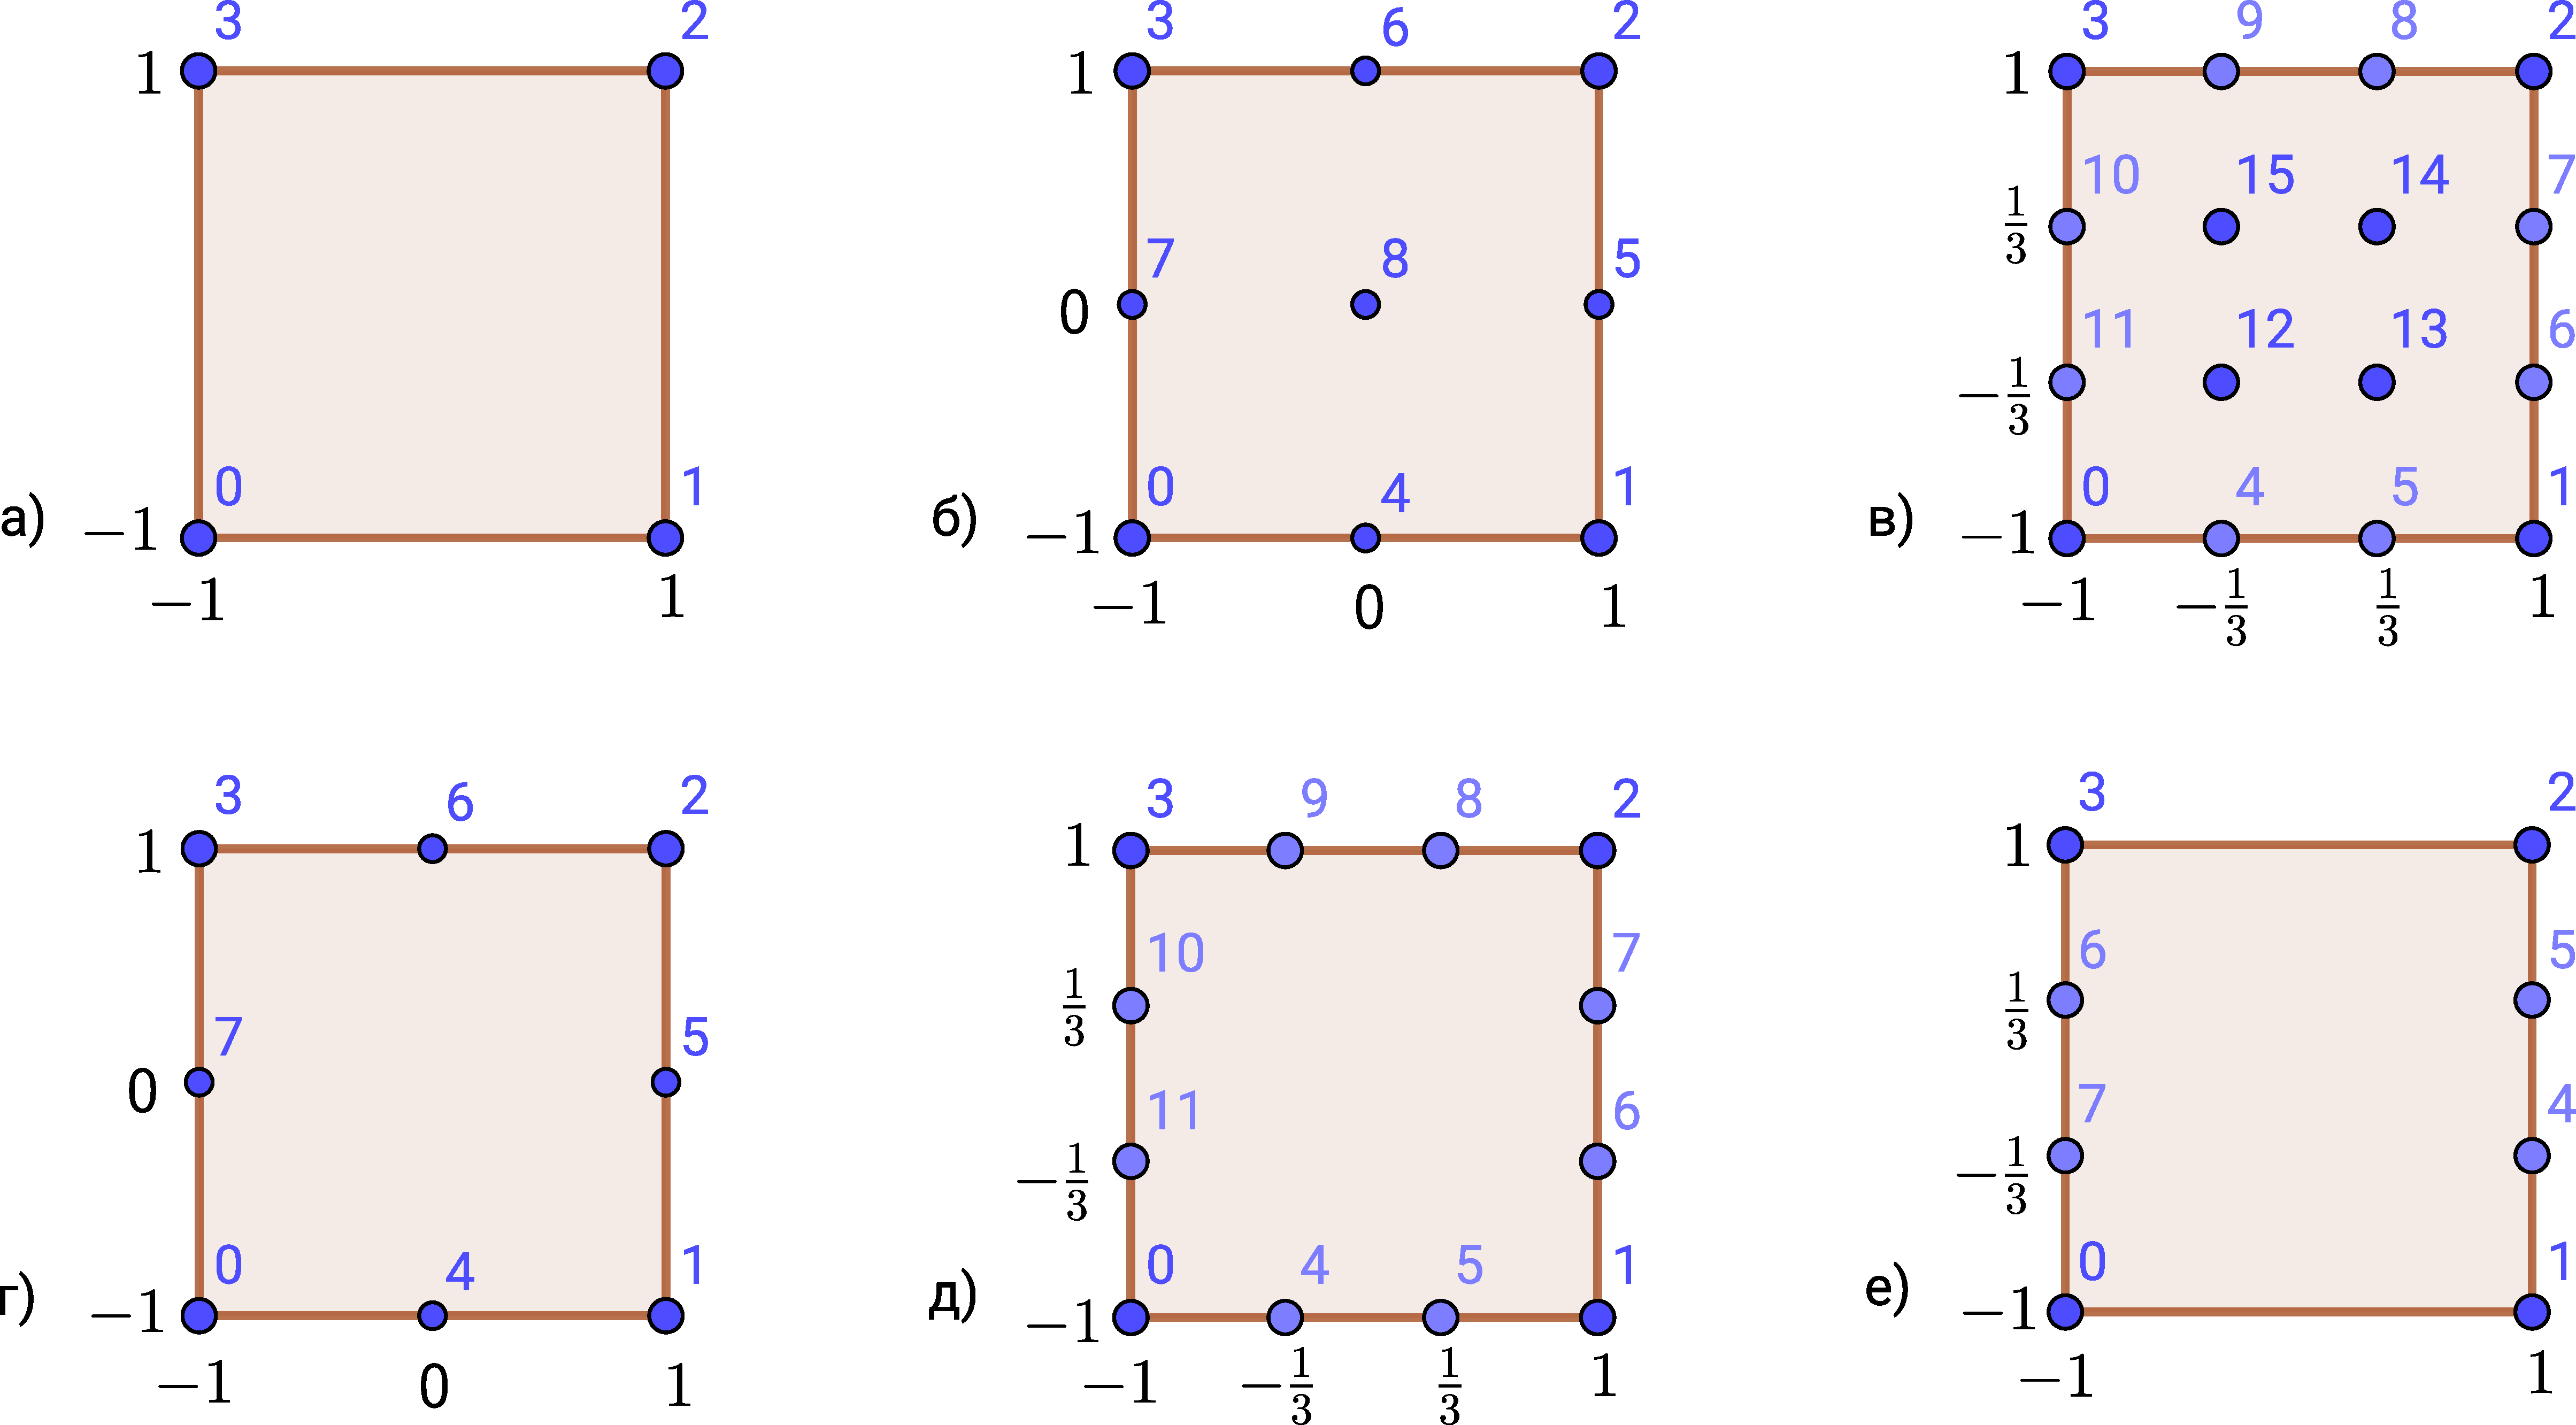
\includegraphics[width=0.7\linewidth]{quadrangle_basis_points.pdf}
\caption{Расположение узловых точек в параметрическом квадратре}
\label{fig:quadrangle_basis_points}
\end{figure}

\paragraph{Билинейный базис}
\begin{equation*}
\phi_i = A^{00}_i + A^{10}_i \xi + A^{01}_i \eta + A^{11}_i \xi\eta.
\end{equation*}

\begin{equation*}
C = \left(
\begin{array}{l|rrrr}
                      & A^{(00)} & A^{(10)} & A^{(01)} & A^{(11)} \\
\hline
\phi(-1, -1) & 1 & -1  & -1   &  1      \\[5pt] 
\phi( 1, -1) & 1 &  1  & -1   & -1      \\[5pt]
\phi( 1,  1) & 1 &  1  &  1   &  1      \\[5pt]
\phi(-1,  1) & 1 & -1  &  1   & -1      \\[5pt]
\end{array}
\right)
\hence
A = C^{-1} = \frac14\left(
\begin{array}{l|rrrr}
        & \phi_0 & \phi_1 & \phi_2 & \phi_3\\
\hline
1       & 1 & 1 & 1 & 1\\[5pt]
\xi     & -1 & 1 & 1 & -1\\[5pt]
\eta    & -1 & -1 & 1 & 1\\[5pt]
\xi\eta & 1 & -1 & 1 & -1
\end{array}
\right)
\end{equation*}

\begin{equation}
\label{eq:quadrangle_bilinear_basis}
\begin{aligned}
&\phi_0(\xi, \eta) = \frac{1-\xi-\eta+\xi\eta}{4}\\[10pt]
&\phi_1(\xi, \eta) = \frac{1+\xi-\eta-\xi\eta}{4}\\[10pt]
&\phi_2(\xi, \eta) = \frac{1+\xi+\eta+\xi\eta}{4}\\[10pt]
&\phi_3(\xi, \eta) = \frac{1-\xi+\eta-\xi\eta}{4}
\end{aligned}
\end{equation}

\begin{figure}[h!]
\centering
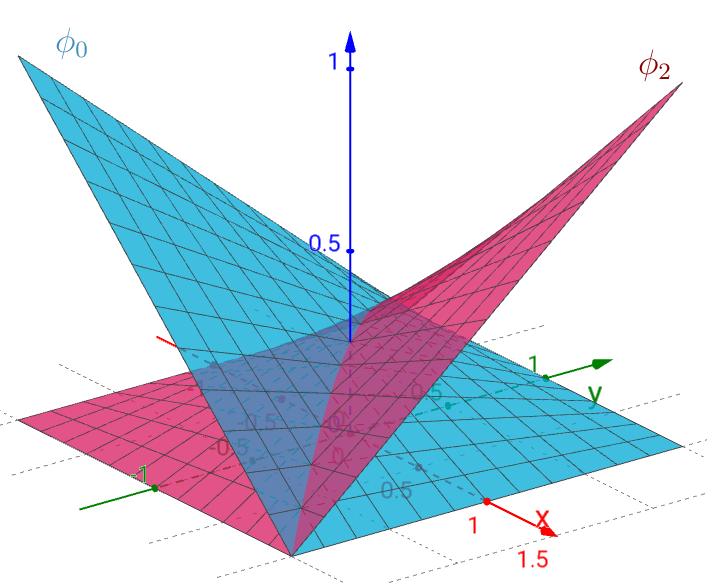
\includegraphics[width=0.4\linewidth]{basis2d_bilinear.png}
\caption{Билинейные функции $\phi_0$, $\phi_2$ в параметрическом квадрате}
\label{fig:basis2d_bilinear}
\end{figure}

\paragraph{Определение двумерных базисов через комбинацию одномерных}
Обратим внимание, что в искомые билинейные базисные функции линейны
в каждом из направлений $\xi, \eta$, если брать их по отдельности.
Значит можно представить эти функции как комбинацию одномерных
линейных базисов \cref{eq:segment_linear_basis} в каждом из направлений.
Узлы двумерного параметрического квадрата можно
выразить через узлы линейного базиса в параметрическом одномерном сегменте,
рассмотренном в п.~\ref{sec:segment_bases}:
$$
\vec \xi_0 = \left(\xi^{1D}_0, \xi^{1D}_0\right), \quad
\vec \xi_1 = \left(\xi^{1D}_1, \xi^{1D}_0\right), \quad
\vec \xi_2 = \left(\xi^{1D}_1, \xi^{1D}_1\right), \quad
\vec \xi_3 = \left(\xi^{1D}_0, \xi^{1D}_1\right).
$$
Значит и соответствующие базисные функции можно выразить
через линейный одномерный базис $\phi^{1D}$ из соотношений \cref{eq:segment_linear_basis}:
\begin{equation*}
\begin{aligned}
\phi_0(\xi, \eta) = \phi_0^{1D}(\xi)\phi^{1D}_0(\eta) = \frac{1-\xi}{2}\frac{1-\eta}{2},\\[5pt]
\phi_1(\xi, \eta) = \phi_1^{1D}(\xi)\phi^{1D}_0(\eta) = \frac{1+\xi}{2}\frac{1-\eta}{2},\\[5pt]
\phi_2(\xi, \eta) = \phi_1^{1D}(\xi)\phi^{1D}_1(\eta) = \frac{1+\xi}{2}\frac{1+\eta}{2},\\[5pt]
\phi_3(\xi, \eta) = \phi_0^{1D}(\xi)\phi^{1D}_1(\eta) = \frac{1-\xi}{2}\frac{1+\eta}{2}.
\end{aligned}
\end{equation*}
Раскрыв скобки можно убедится, что мы получили тот же билинейный базис, что и ранее \cref{eq:quadrangle_bilinear_basis}.

\paragraph{Биквадратичный базис}
Применим этот метод для вычисления биквадратичного базиса, определённого в точках на \figref{fig:quadrangle_basis_points}б.
В качестве основе возьмём квадратичный одномерный базис $\phi^{1D}_i$ из \cref{eq:segment_quadratic_basis}.
\begin{equation}
\label{eq:quadrangle_quadratic_basis}
\begin{array}{ll}
  \phi_0(\xi, \eta) = \phi_0^{1D}(\xi)\phi_0^{1D}(\eta) = \dfrac{\xi^2 - \xi}{2}\dfrac{\eta^2 - \eta}{2},
& \phi_1(\xi, \eta) = \phi_1^{1D}(\xi)\phi_0^{1D}(\eta) = \dfrac{\xi^2 + \xi}{2}\dfrac{\eta^2 - \eta}{2}, \\[10pt]
  \phi_2(\xi, \eta) = \phi_1^{1D}(\xi)\phi_1^{1D}(\eta) = \dfrac{\xi^2 + \xi}{2}\dfrac{\eta^2 + \eta}{2},
& \phi_3(\xi, \eta) = \phi_0^{1D}(\xi)\phi_1^{1D}(\eta) = \dfrac{\xi^2 - \xi}{2}\dfrac{\eta^2 + \eta}{2}, \\[10pt]
  \phi_4(\xi, \eta) = \phi_2^{1D}(\xi)\phi_0^{1D}(\eta) = (1-\xi^2)\dfrac{\eta^2 - \eta}{2},
& \phi_5(\xi, \eta) = \phi_1^{1D}(\xi)\phi_2^{1D}(\eta) = \dfrac{\xi^2 + \xi}{2}(1 - \eta^2),            \\[10pt]
  \phi_6(\xi, \eta) = \phi_2^{1D}(\xi)\phi_1^{1D}(\eta) = (1-\xi^2)\dfrac{\eta^2 + \eta}{2},
& \phi_7(\xi, \eta) = \phi_0^{1D}(\xi)\phi_2^{1D}(\eta) = \dfrac{\xi^2 - \xi}{2}(1 - \eta^2),            \\[10pt]
  \phi_8(\xi, \eta) = \phi_2^{1D}(\xi)\phi_2^{1D}(\eta) = (1-\xi^2)(1 - \eta^2).
&
\end{array}
\end{equation}

\paragraph{Бикубический базис}

\paragraph{Неполный биквадратичный базис}

\paragraph{Неполный бикубический базис}


\section{Алгоритмы}
\subsection{Геометрические алгоритмы}
\subsubsection{Линейная интерполяция}
\begin{figure}[h!]
\centering
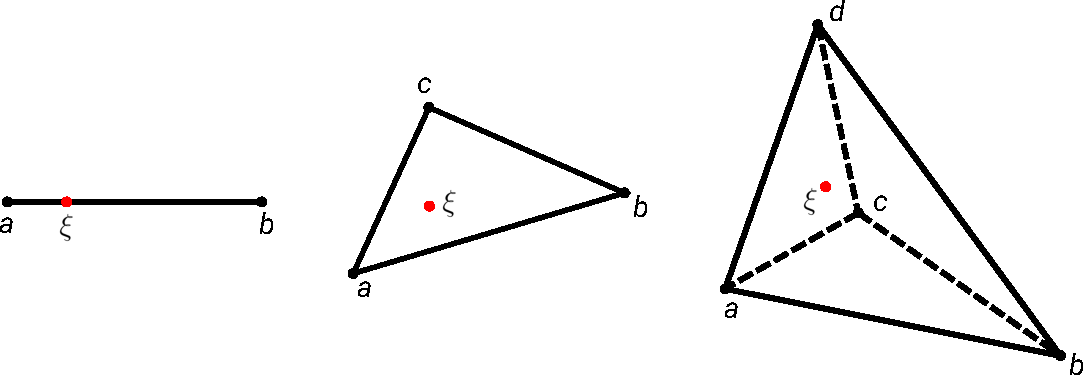
\includegraphics[width=0.8\linewidth]{geom_interp.pdf}
\caption{Порядок нумерации точек одномерного, двумерного и трёхмерного симплекса при линейной интерполяции}
\label{fig:geom_interp}
\end{figure}
Пусть функция $u$ задана в узлах симплекса, имеющего нумерацию согласно рис.~\ref{fig:geom_interp}.
Необходимо найти значение этой функции в точке $\vec \xi$ (эта точка вообще говоря не обязана лежать внутри симлекса).

Интерполяция в одномерном, двумерном и трёхмерном виде запишется как
\begin{align}
\label{eq:simplex_interp_1d}
&u(\xi) =
\frac{
|\triangle_{\xi a}|u(b)+
|\triangle_{b \xi}|u(a)
}
{|\triangle_{ba}|}
\\[10pt]
\label{eq:simplex_interp_2d}
&u(\xi) =
\frac{
|\triangle_{ab\xi}|u(c) +
|\triangle_{bc\xi}|u(a) +
|\triangle_{ca\xi}|u(b)
}
{|\triangle_{abc}|}
\\[10pt]
\label{eq:simplex_interp_3d}
&u(\xi) =
\frac{
|\triangle_{abc\xi}|u(d) +
|\triangle_{cbd\xi}|u(a) +
|\triangle_{cda\xi}|u(b) +
|\triangle_{adb\xi}|u(c)
}
{|\triangle_{abcd}|},
\end{align}
где $|\triangle|$ -- знаковый объём симплекса, вычисляемый как
\begin{align*}
& |\triangle_{ab}| = b - a, \\[10pt]
& |\triangle_{abc}| = \left(\frac{(\vec b - \vec a)\times(\vec c - \vec a)}{2}\right)_z, \\[10pt]
& |\triangle_{abcd}| = \frac{(\vec b - \vec a)\cdot\left((\vec c - \vec a)\times(\vec d - \vec a)\right)}{6}.\\[10pt]
\end{align*}

\subsubsection{Преобразование координат}
\label{sec:coo_transform} 
Рассмотрим преобразование
из двумерной параметрической системы координат $\vec \xi$ 
в физическую систему $\vec x$.
Такое преобразование полностью определяется покоординатными
функциями $\vec x(\vec \xi)$.
Далее получим соотношения, связывающие операции дифференцирования
и интегрирования в физической и параметрической областях.

\subsubsubsection{Матрица Якоби}
Будем рассматривать двумерное преобразование $(\xi, \eta) \to (x, y)$.
Линеаризуем это преобразование (разложим в ряд Фурье до линейного слагаемого)
\begin{align*}
& x(\xi_0 + d\xi, \eta_0 + d\eta) \approx x_0 + \left.\dfr{x}{\xi}\right|_{\xi_0, \eta_0} d\xi
    + \left.\dfr{x}{\eta}\right|_{\xi_0, \eta_0} d\eta, \\
& y(\xi_0 + d\xi, \eta_0 + d\eta) \approx y_0 + \left.\dfr{y}{\xi}\right|_{\xi_0, \eta_0} d\xi
    + \left.\dfr{y}{\eta}\right|_{\xi_0, \eta_0} d\eta,
\end{align*}
где $x_0 = x(\xi_0, \eta_0)$, $y_0 = y(\xi_0, \eta_0)$.
Переписывая это выражение в векторном виде, получим
\begin{equation}
\label{eq:jacobi_linear}
\vec{x}(\vec \xi_0 + \vec{d\xi} ) - \vec{x}_0 = J(\vec \xi_0) \; \vec{d\xi}.
\end{equation}
Матрица $J$ (зависящая от точки приложения в параметрической плоскости) называется матрицей Якоби:
\begin{equation}
\label{eq:jacobi_matrix_2d}
J = \left(
	\begin{array}{cc}
	J_{11} & J_{12}\\[10pt]
	J_{21} & J_{22}\\
	\end{array}
\right)
= \left(
	\begin{array}{cc}
	\ddfr{x}{\xi} & \ddfr{x}{\eta}\\[10pt]
	\ddfr{y}{\xi} & \ddfr{y}{\eta}\\
	\end{array}
\right)
\end{equation}

\paragraph{Якобиан}

\begin{figure}[h!]
\centering
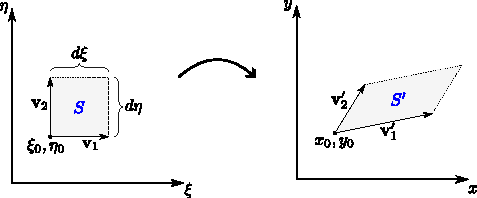
\includegraphics[width=0.6\linewidth]{dxideta.pdf}
\caption{Преобразование элементарного объёма}
\label{fig:dxideta}
\end{figure}

Определитель матрицы Якоби (якобиан), взятый в конкретной точке параметрической плоскости $\vec\xi_0$, показывает,
во сколько раз увеличился элементарный объём около этой точки в результате преобразования.
Действительно, рассмотрим два перпендикулярных элементарных вектора
в параметрической системе координат: $\vec v_1 = (d\xi, 0)$ и $\vec v_2 = (0, d\eta)$
отложенных от точки $\vec\xi_0$ (см.~\figref{fig:dxideta}).
В результате преобразования по формуле \cref{eq:jacobi_linear} 
получим следующие преобразования концевых точек и векторов:
\begin{align*}
& (\xi_0, \eta_0) \to (x_0, y_0), \\
& (\xi_0 + d\xi, \eta_0) \to (x_0 + J_{11} d\xi, y_0 + J_{21} d\xi) \hence \vec v_1 \to \vec v'_1 = (J_{11} d\xi, J_{21} d\xi), \\
& (\xi_0 , \eta_0 + d\eta) \to (x_0 + J_{12} d\eta, y_0 + J_{22} d\eta) \hence \vec v_2 \to \vec v'_2 = (J_{12} d\eta, J_{22} d\eta).
\end{align*}
Элементарный объём равен площади параллелограмма, построенного
на элементарных векторах.
В параметрической плоскости согласно \cref{eq:vec_cross_2d} получим 
$$ |S| = \vec v_1 \times \vec v_2 = d\xi d\eta,$$
и аналогично для физической плоскости:
$$
|S'| = \vec v'_1 \times \vec v'_2 = (J_{11} J_{22} - J_{12} J_{21})d\xi d\eta = |J| d\xi d\eta
$$
Сравнивая два последних соотношения приходим к выводу,
что элементарный объём в результате преобразования увеличился в $|J|$ раз. Тогда можно записать
\begin{equation}
\label{eq:dxdy_dxideta}
dx\,dy = |J|\,d\xi\,d\eta
\end{equation}

Многомерным обобщением этой формулы будет
\begin{equation}
\label{eq:vec_dx_dxi}
d\vec x = |J|\,d\vec \xi
\end{equation}

\subsubsubsection{Дифференцирование в параметрической плоскости}
Пусть задана некоторая функция $f(x, y)$. Распишем её производную по
параметрическим координатам:
\begin{align*}
&\dfr{f}{\xi} = \dfr{f}{x}\dfr{x}{\xi} + \dfr{f}{y}\dfr{y}{\xi}, \\
&\dfr{f}{\eta} = \dfr{f}{x}\dfr{x}{\eta} + \dfr{f}{y}\dfr{y}{\eta}.
\end{align*}
Вспоминая определение \cref{eq:jacobi_matrix_2d}, запишем
\begin{equation*}
\left(\begin{array}{c}
  \ddfr{f}{\xi} \\[10pt]
  \ddfr{f}{\eta}
  \end{array}
\right) = 
J^T 
\left(
  \begin{array}{c}
  \ddfr{f}{x} \\[10pt]
  \ddfr{f}{y}
  \end{array}
\right) =
\left(
  \begin{array}{cc}
    J_{11} & J_{21} \\[10pt]
    J_{12} & J_{22}
  \end{array}
\right)
\left(
  \begin{array}{c}
  \ddfr{f}{\xi} \\[10pt]
  \ddfr{f}{\eta}
  \end{array}
\right)
\end{equation*}
Обратная зависимость примет вид
\begin{equation*}
\left(\begin{array}{c}
  \ddfr{f}{x} \\[10pt]
  \ddfr{f}{y}
  \end{array}
\right) = 
\left(J^T\right)^{-1}
\left(
  \begin{array}{c}
  \ddfr{f}{\xi} \\[10pt]
  \ddfr{f}{\eta}
  \end{array}
\right) =
\frac{1}{|J|}
\left(
  \begin{array}{cc}
    J_{22} & -J_{21} \\[10pt]
    -J_{12} & J_{11}
  \end{array}
\right)
\left(
  \begin{array}{c}
  \ddfr{f}{\xi} \\[10pt]
  \ddfr{f}{\eta}
  \end{array}
\right)
\end{equation*}
В многомерном виде запишем
\begin{equation}
\label{eq:vec_grad_dx}
\nabla_{\vec x} f = \left(J^T\right)^{-1} \nabla_{\vec \xi} f.
\end{equation}

\subsubsubsection{Интегрирование в параметрической плоскости}
Пусть в физической области $\vec x$ задана область $D_x$.
Интеграл функции $f(\vec x)$ по этой области
можно расписать, используя замену \cref{eq:vec_dx_dxi}
\begin{equation}
\label{eq:dxideta_integral}
\int\limits_{D_{x}}f(\vec x)\,d\vec x = \int\limits_{D_{\xi}}f(\vec \xi) \, |J(\vec \xi)|d\vec \xi,
\end{equation}
где $f(\vec \xi) = f(\vec x(\vec \xi))$, а $D_\xi$ -- образ области $D_x$ в параметрической плоскости.

\subsubsubsection{Двумерное линейное преобразование. Параметрический треугольник}
\label{sec:lintri_transform}
\begin{figure}[h!]
\centering
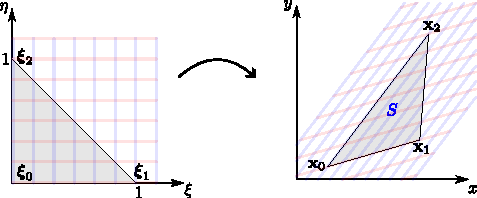
\includegraphics[width=0.6\linewidth]{lintri_transform.pdf}
\caption{Преобразование из параметрического треугольника}
\label{fig:lintri_transform}
\end{figure}
Рассмотрим двумерное преобразование, при котором
определяющие функции являются линейными. То есть представимыми в виде
\begin{align*}
x(\xi, \eta) = A_x \xi + B_x \eta + C_x, \\
y(\xi, \eta) = A_y \xi + B_y \eta + C_y.
\end{align*}
Для определения шести констант, определяющих это преобразование,
достаточно выбрать три любые (не лежащие на одной прямой) точки:
$(\xi_i, \eta_i) \to (x_i, y_i)$ для $i=0,1,2$.
В результате получим систему из шести линейных уравнений (три точки по две координаты),
из которой находятся конcтанты $A_{x,y}, B_{x,y}, C_{x,y}$.
Пусть три точки в параметрической плоскости
образуют единичный прямоугольный треугольник (\figref{fig:lintri_transform}):
\begin{equation*}
\xi_0, \eta_0 = (0, 0),\quad
\xi_1, \eta_1 = (1, 0),\quad
\xi_2, \eta_2 = (0, 1).
\end{equation*}
Тогда система линейных уравнений примет вид
\begin{align*}
&x_0 = C_x,       \quad y_0 = C_y, \\
&x_1 = A_x + C_x, \quad y_1 = A_y + C_y, \\
&y_2 = B_x + C_x, \quad y_2 = B_y + C_y.
\end{align*}
Определив коэффициенты преобразования их этой системы, окончательно запишем преобразование
\begin{equation}
\label{eq:lintri_transform}
\begin{aligned}
&x(\xi, \eta) = (x_1 - x_0)\xi + (x_2 - x_0) \eta + x_0,\\
&y(\xi, \eta) = (y_1 - y_0)\xi + (y_2 - y_0) \eta + y_0.\\
\end{aligned}
\end{equation}
Матрица Якоби этого преобразования \cref{eq:jacobi_matrix_2d}
не будет зависеть от параметрических координат $\xi, \eta$:
\begin{equation}
\label{eq:lintri_jacobi_matrix}
J = \left(
\begin{array}{cc}
x_1 - x_0 & x_2 - x_0 \\
y_1 - y_0 & y_2 - y_0 \\
\end{array}
\right).
\end{equation}
Якобиан преобразования будет равен удвоенной площади треугольника $S$, составленного из определяющих точек в физической плоскости:
\begin{equation}
\label{eq:lintri_jacobian}
|J| = (x_1 - x_0) (y_2 - y_0) - (y_1 - y_0) (x_2 - x_0) = (\vec x_1 - \vec x_0) \times (\vec x_2 - \vec x_0) = 2 |S|.
\end{equation}
Распишем интеграл по треугольнику $S$ по формуле \cref{eq:dxideta_integral}.
Вследствии линейности преобразования якобиан постоянен и, поэтому, его можно вынести его из-под интеграла:
\begin{equation}
\label{eq:lintri_integral}
\int\limits_{S}f(x, y)\,dxdy = |J|\int\limits_0^1 \int\limits_0^{1-\xi} f(\xi, \eta) d\eta d\xi.
\end{equation}

\subsubsubsection{Двумерное билинейное преобразование. Параметрический квадрат}
\label{sec:bilinquad_transform}
\begin{figure}[h!]
\centering
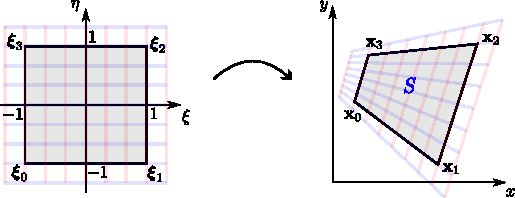
\includegraphics[width=0.6\linewidth]{bilinquad_transform.pdf}
\caption{Преобразование из параметрического квадрата}
\label{fig:bilinquad_transform}
\end{figure}

\subsubsubsection{Трёхмерное линейное преобразование. Параметрический тетраэдр}
TODO

\subsubsection{Свойства многоугольника}
\subsubsubsection{Площадь многоугольника}
\label{sec:polygon_area} 

\begin{figure}[h!]
\centering
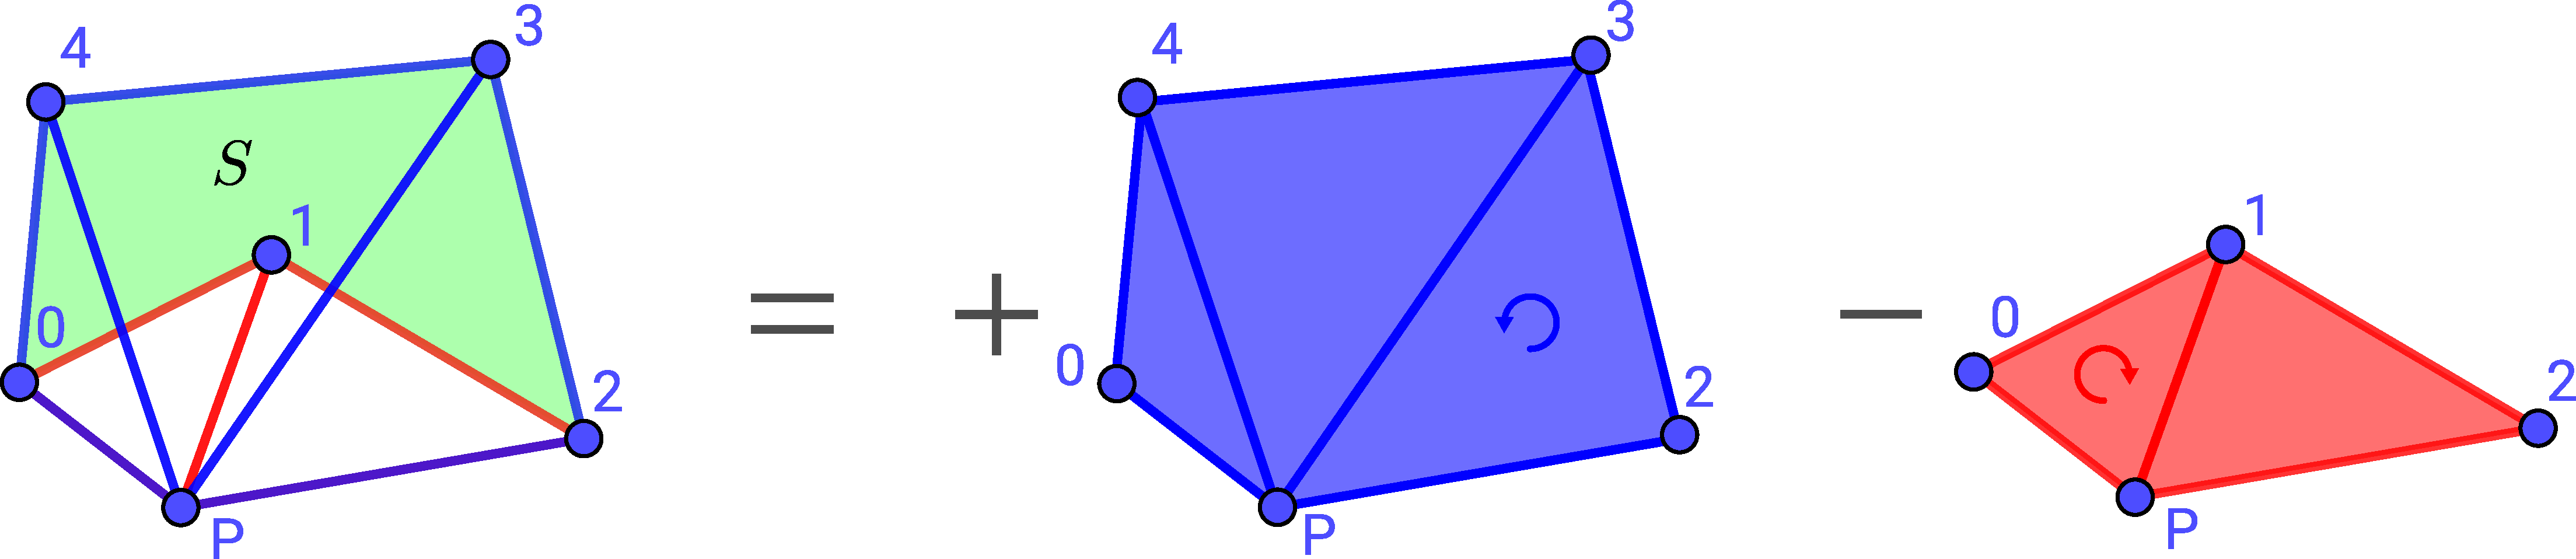
\includegraphics[width=0.7\linewidth]{polygon_area.pdf}
\caption{Площадь произвольного многоугольника}
\label{fig:polygon_area}
\end{figure}

Рассмотрим произвольный несамопересекающийся $N$-угольник $S$,
заданный координатами своих узлов $\vec x_i$, $i=\overline{0, N-1}$,
пронумерованных последовательно против часовой стрелки (\figref{fig:polygon_area}).
Далее введём произвольную точку $\vec p$ и 
от этой точки будем строить ориентированные треугольники до граней многоугольника:
$$
\triangle^p_i = (\vec p, \vec x_i, \vec x_{i+1}), \quad i=\overline{0, N-1},
$$
(для корректности записи будем считать, что $\vec x_N = \vec x_0$).
Тогда площадь исходного многоугольника $S$ будет равна сумме
знаковых площадей треугольников $\triangle^p_i$:
$$
|S| = \sum_{i=0}^{N-1} |\triangle^p_i|, \qquad |\triangle^p_i| = \frac{(\vec x_i - \vec p) \times (\vec x_{i+1} - \vec p)}{2}.
$$
Знак площади ориентированного треугольника зависит от направления закрутки его узлов:
она положительна для закрутки против часовой стрелки и отрицательна, если узлы пронумерованы по часовой стрелке.
В частности, на рисунке~\ref{fig:polygon_area} видно, что треугольники, отмеченные красным: $P01, P12$, будут
иметь отрицательную площадь, а синие треугольники $P23$, $P34$, $P40$ -- положительную. Сумма этих площадей
с учётом знака даст искомую площадь многоугольника.

Для сокращения вычислений воспользуемся произвольностью положения $\vec p$ и совместим
её с точкой $\vec x_0$. Тогда треугольники $\triangle^p_0$, $\triangle^p_{N-1}$
выродятся (будут иметь нулевую площадь).
Обозначим такую последовательную триангуляцию как
\begin{equation}
\label{eq:seq_polygon_triangulation}
\triangle_i = (\vec x_0, \vec x_i, \vec x_{i+1}), \qquad i=\overline{1,N-2}.
\end{equation}
Знаковая площадь ориентированного треугольника будет равна
\begin{equation}
\label{eq:seq_triangle_area}
|\triangle_i| = \frac{(\vec x_i - \vec x_0) \times (\vec x_{i+1} - \vec x_0)}{2}.
\end{equation}
Тогда окончательно формула определения площади примет вид
\begin{equation}
\label{eq:polygon_area}
|S| = \sum_{i=1}^{N-2}|\triangle_i|.
\end{equation}

\paragraph{Плоский полигон в пространтве} Если плоский полигон $S$ расположен в трёхмерном пространстве,
то правая часть формулы \cref{eq:seq_triangle_area} согласно определению векторного произведения в трёхмерном пространстве \cref{eq:vec_cross}
-- есть вектор.
Чтобы получить скалярную площадь, нужно спроецировать этот вектор на единичную нормаль к плоскости
многоугольника:
$$
\vec n = \frac{\vec k}{|\vec k|}, \qquad \vec k = (\vec x_1 - \vec x_0) \times (\vec x_2 - \vec x_0).
$$
Эта формула записана из предположения, что узел $\vec x_2$ не лежит
на одной прямой с узлами $\vec x_0$, $\vec x_1$. Иначе вместо $\vec x_2$ нужно
выбрать любой другой узел, удовлетворяющий этому условию.
Тогда площадь ориентированного треугольника, построенного
в трёхмерном пространстве запишется через смешанное произведение:
\begin{equation}
\label{eq:seq_triangle_area_3d}
|\triangle_i| = \frac{\left((\vec x_i - \vec x_0) \times (\vec x_{i+1} - \vec x_0) \right)\cdot \vec n}{2}.
\end{equation}
Формула для определения площади полигона \cref{eq:polygon_area} будет по прежнему верна.
При этом итоговый знак величины $S$ будет положительным,
если закрутка полигона положительная (против часовой стрелки) при взгляде со стороны
вычисленной нормали $\vec n$.

\subsubsubsection{Интеграл по многоугольнику}
\label{sec:polygon_integral} 
Рассмотрим интеграл функции $f(x,y)$ по $N$-угольнику $S$, заданному последовательными координатами своих узлов $\vec x_i$.
Введём последовательную триангуляцию согласно \cref{eq:seq_polygon_triangulation}.
Тогда интеграл по многоугольнику можно расписать как сумму интегралов по ориентированным треугольникам:
\begin{equation}
\label{eq:seq_triangulation_integral}
\arint{f(x,y)}{S}{xdy} = \sum_{i=1}^{N-2} \arint{f(x,y)}{\triangle_i}{xdy}.
\end{equation}
Далее для вычисления интегралов в правой части
воспользуемся преобразованием к параметрическому треугольнику (п.~\ref{sec:lintri_transform}).
Следуя формуле интегрирования \cref{eq:lintri_integral}, распишем
интеграл по $i$-ому треугольнику:
\begin{equation*}
\arint{f(x,y)}{\triangle_i}{xdy} = |J_i| \int\limits_{0}^{1}\int\limits_{0}^{1-\xi} f_i(\xi, \eta) \, d\eta d\xi,
\end{equation*}
где якобиан $|J_i|$ согласно \cref{eq:lintri_jacobian} есть удвоенная площадь ориентированного треугольника $\triangle_i$
(положительная при закрутке против часовой стрелке и отрицаетельная иначе):
\begin{equation*}
|J_i| = 2|\triangle_i| = (\vec x_i - \vec x_0) \times (\vec x_{i+1} - \vec x_0),
\end{equation*}
а функция $f_i(\xi, \eta)$ есть функция от преобразованных согласно \cref{eq:lintri_transform}
переменных:
\begin{equation*}
f_i(\xi, \eta) = f\left(\left(\vec x_i - \vec x_0\right)\xi + \left(\vec x_{i+1} - \vec x_0\right)\eta + \vec x_0\right).
\end{equation*}
Окончательно запишем
\begin{equation}
\label{eq:polygon_integral}
\arint{f(x,y)}{S}{xdy} = 2 \sum_{i=1}^{N-2}
    |\triangle_i| \int\limits_{0}^{1}\int\limits_{0}^{1-\xi} f_i(\xi, \eta) \, d\eta d\xi.
\end{equation}
Отметим, что эта формула работает и в том случае, когда
полигон расположен в трёхмерном пространстве
(знаковую площадь при этом следует вычислять по \cref{eq:seq_triangle_area_3d}).

\subsubsubsection{Центр масс многоугольника}
\label{sec:polygon_center} 
По определению, координаты центра масс $\vec c$ области $S$ равны среднеинтегральным значениям координатных функций. То есть
\begin{equation*}
c_x = \frac{1}{|S|}\int\limits_{S} x \, dxdy,
\quad 
c_y = \frac{1}{|S|}\int\limits_{S} y \, dxdy.
\end{equation*}
Далее распишем интеграл в правой части через последовательную триангуляцию согласно
\cref{eq:seq_triangulation_integral} с учётом линейного преобразования
\cref{eq:lintri_transform}:
\begin{align*}
\int\limits_{S} x \, dxdy &= \sum_{i=1}^{N-2} \int\limits_{\triangle_i} x \, dxdy\\
                          &= \sum_{i=1}^{N-2} |J_i| \int\limits_0^1\int\limits_0^{1-\xi} ((x_i - x_0)\xi + (x_{i+1} - x_0)\eta + x_0)\, d\eta d\xi\\
                          &= \sum_{i=1}^{N-2} \frac{|J_i|}{2}\frac{x_0 + x_i + x_{i+1}}{3}\\
                          &= \sum_{i=1}^{N-2} |\triangle_i|\frac{x_0 + x_i + x_{i+1}}{3}.
\end{align*}
Итого, с учётом \cref{eq:polygon_area}, координаты центра масс примут вид
\begin{align*}
&\vec c = \dfrac{\displaystyle\sum_{i=1}^{N-2} \dfrac{\vec x_0 + \vec x_i + \vec x_{i+1}}{3}|\triangle_i|}{\displaystyle\sum_{i=1}^{N-2} |\triangle_i|}.
\end{align*}
Если полигон расположен в двумерном пространстве $xy$, то знаковая площадь треугольников
вычисляется по формуле \cref{eq:seq_triangle_area}.
В случае трёхмерного пространтва должна использоваться формула \cref{eq:seq_triangle_area_3d}.

\subsubsection{Свойства многогранника}
\subsubsubsection{Объём многогранника}
\label{sec:polyhedron_volume} 
TODO
\subsubsubsection{Интеграл по многограннику}
\label{sec:polyhedron_integral} 
TODO
\subsubsubsection{Центр масс многогранника}
\label{sec:polyhedron_center} 
TODO

\subsubsection{Поиск многоугольника, содержащего заданную точку}
TODO

\subsection{Форматы хранения разреженных матриц}
\label{sec:sparse-matrix}
\subsubsection{CSR-формат}
\label{sec:csr}
При реализации решателей систем сеточных уравнений важно учитывать
разреженный характер используемых в левой части. То есть избегать
хранения и ненужных операций с нулевыми элементами матрицы.

Хотя рассмотренные ранее алогритмы конечноразностных аппроксимаций на структурированных сетках
давали трёх- (для одномерных задач) или пятидиагональную (для двумерных) сеточную матрицу,
здесь будем рассматривать общие форматы хранения, не привязанные к конкретному шаблону.

Любой общий
формат хранения должен хранить
информацию о шаблоне матрице (адресах ненулевых элементов)
и значениях матричных коэффициентов в этом шаблоне.

В CSR (Compressed sparse rows) формате
все ненулевые элементы хранятся в линейном массиве \ename{vals}.
А шаблон матрицы -- в двух массивах
\begin{itemize}
	\item массиве колонок \ename{cols} -- значений колонок для соответствующих ему значений из массива \ename{vals},
	\item массиве адресов \ename{addr} -- индексах массива \ename{vals}, с которых начинается описание соответствующей строки.
\end{itemize}
В конце массива \ename{addr} добавляется общая длина массива \ename{vals}.

Таким образом, длины массивов \ename{vals}, \ename{cols} равны количеству ненулевых элементов матрицы,
а длина массива \ename{addr} равна количеству строк в матрице плюс один.

Для облегчения процедур поиска описание каждой строки должно идти последовательно
с увеличением индекса колонки.

Для примера рассмотрим следующую матрицу
\begin{equation}
\label{eq:example-sparse-matrix}
\left(
\begin{array}{cccc}
2.0 & 0 & 0 & 1.0 \\
0 & 3.0 & 5.0 & 4.0 \\
0 & 0 & 6.0 & 0 \\
0 & 7.0 & 0 & 8.0 \\
\end{array}
\right)
\end{equation}

Массивы, описывающие матрицу в формате CSR примут вид

\begin{equation*}
\begin{array}{r|l|l|l|l|l}
      & row=0     & row=1          & row=2& row=3&\\
\hline
vals= & 2.0, 1.0, & 3.0, 5.0, 4.0, & 6.0, & 7.0, 8.0 &\\
\hline
cols= & 0,\phantom{.0} 3,\phantom{.0}      & 1,\phantom{.0}2,\phantom{.0}3,\phantom{.0}          & 2,\phantom{.0}   & 1,\phantom{.0} 3     &\\
\hline
addr= & 0,        & 2,             & 5,   & 6,       & 8 \\
\hline
\end{array}
\end{equation*}

Рассмотрим реализацию базовых алгоритмов для матриц, заданных в этом формате.

Пусть матрица задана следующими массивами:
\begin{minted}[linenos=false]{c++}
std::vector<double> vals; // массив значений
std::vector<size_t> cols; // массив столбцов
std::vector<size_t> addr; // массив адресов
\end{minted}

Число строк в матрице:
\begin{minted}[linenos=false]{c++}
size_t nrows = addr.size()-1;
\end{minted}

Число элементов в шаблоне (ненулевых элементов)
\begin{minted}[linenos=false]{c++}
size_t n_nonzeros = vals.size();
\end{minted}

Число ненулевых элементов в заданной строке `irow`
\begin{minted}[linenos=false]{c++}
size_t n_nonzeros_in_row = addr[irow+1] - addr[irow];
\end{minted}

Умножение матрицы на вектор `v` (длина этого вектора должна быть равна числу строк в матрице).
Здесь реализуется суммирование вида
\begin{equation*}
    r_i = \sum_{j=0}^{N-1} A_{ij} v_j,
\end{equation*}
при этом избегаются лишние операции с нулями
\begin{minted}[linenos=false]{c++}
// число строк в матрице и длина вектора v
size_t nrows = addr.size() - 1;
// массив ответов. Инициализируем нулями
std::vector<double> r(nrows, 0);
// цикл по строкам
for (size_t irow=0; irow < nrows; ++irow){
	// цикл по ненулевым элементам строки irow
	for (size_t a = addr[irow]; a < addr[irow+1]; ++a){
		// получаем индекс колонки
		size_t icol = cols[a];
		// значение матрицы на позиции [irow, icol]
		double val = vals[a];
		// добавляем к ответу
		r[irow] += val * v[icol];
	}
}
\end{minted}


Поиск значения элемента матрицы по адресу \cvar{(irow, icol)} с учётом локально сортированного вектора \cvar{cols}
\begin{minted}[linenos=false]{c++}
using iter_t = std::vector<size_t>::const_iterator;
// указатели на начало и конец описания строки в массиве cols
iter_t it_start = cols.begin() + addr[irow];
iter_t it_end = cols.begin() + addr[irow+1];
// поиск значения icol в отсортированной последовательности [it_start, it_end)
iter_t fnd = std::lower_bound(it_start, it_end, icol);
if (fnd != it_end && *fnd == icol){
	// если нашли, то определяем индекс найденного элемента в массиве cols
	size_t a = fnd - cols.begin();
	// и возвращаем значение из vals по этому индексу
	return vals[a];
} else {
	// если не нашли, значит элемент [irow, icol] находится вне шаблона. Возвращаем 0
	return 0;
}
\end{minted}

Формат CSR обеспечивает максимальную компактность хранения
разреженной матрицы и при этом удобен для последовательной итерации по элементам матрицы (операции умножения матрицы на вектор),
но его существенным недостатком является высокая сложность добавления нового элемента в шаблон.

\subsubsection{Массив словарей}
При реализации сеточных методов решения дифференциальных уравнений работу с матрицами
можно разбить на два этапа: сборка матриц и их непосредственное использование.
Сборка матрицы в свою очередь может быть разделена на
этап вычисление шаблона матрицы (символьная сборка) и
непосредственное вычисление коэффициентов матрицы (числовая сборка).

На этапе использования матрицы основной операцией
является умножение матрицы на вектор, где наиболее эффективным является CSR-формат.

В случае использования неструктурированных сеток этап символьной сборки
является нетривиальной операцией и сводится к неупорядоченному добавлению
новых элементов в шаблон матрицы. Как было отмечено ранее, 
такая операция в случае использования CSR формата неэффективена.

Поэтому часто для этапов сборки и расчёта используют
разные форматы хранения матриц, первый из которых оптимизирован для операции вставки, а второй -- для операции умножения на вектор.
В качестве формата, оптимизированного для вставки, можно представить формат массива словарей (List of dictionaries), где каждая строка матрицы
описывается словарём, ключём которого является индекс колонки, а значением -- величина соответствующего матричного коэффициента.

С использованием синтаксиса C++ такой формат может быть описан следующим образом:
\begin{cppcode}
std::vector<std::map<size_t, double>> data;
\end{cppcode}

Марица вида \eqref{eq:example-sparse-matrix} в таком формате примет вид
\begin{cppcode}
data = {
	{0: 2.0, 3: 1.0},
	{1: 3.0, 2: 5.0, 3: 4.0},
	{2: 6.0},
	{1: 7.0, 3: 8.0}
};
\end{cppcode}

Добавление нового матричного коэффициента сведётся к вставке элемента в словарь:
\begin{cppcode}
data[i][j] = value;
\end{cppcode}

А основной операцией для такого формата будет служить
конверсия в CSR:
\begin{cppcode}
std::vector<size_t> addr{0};
std::vector<size_t> cols;
std::vector<double> vals;
for (size_t irow=0; irow < data.size(); ++irow){
	for (auto it: data[irow]){
		cols.push_back(it.first);
		vals.push_back(it.second);
	}
	addr.push_back(addr.back() + data[irow].size());
}
\end{cppcode}
Поскольку данные в контейнере типа \cvar{std::map} итерируются
в отсортированном по ключам порядке, то полученный
в результе массив \cvar{cols} также является локально отсортированным.


\section{Работа с инфраструктурой проекта CFDCourse}
В настоящем параграфе будут даны инструкции для разворачивания инфраструктуры сборки проекта
для операционных систем Linux(Ubuntu), MacOS и Windows.

В процессе настройки будет необходимо установить систему контроля версий {\bf Git},
систему контейнеризации {\bf Docker} и (опционально) интегрированную среду разработки.
Проект позволяет работать в любой среде разработки.
Ниже будут приведены инструкции для настройки {\bf vscode}.

Процесс сборки и запуска программ будет осуществляться в системе, развёрнутой в докере на основе Ubuntu 24.04.
В дальнейшем систему, установленную непосредственно на компьютере, будем называть хост системой.
А систему, развёрнутую в докере -- контейнером.

Для успешной установке на хосте должно быть около 5Гб свободного места.

\subsection{Клонирование}
Для клонирования проекта на локальный компьютер необходимо установить систему контроля версий Git
и открыть терминал на хост-системе в папке, в которой планируется хранить папку с репозиторием.
В нижеследующих инструкциях в качестве такой папки будет использоваться домашняя папка пользователя.

\begin{center}

\begin{tcolorbox}[osstyle, title=Ubuntu]
Откройте терминал и в нём
\begin{shelloutput}
sudo apt install git  # установка гита
cd ~                  # переходим в папку,
                      # где будет хранится папка с репозиторием
\end{shelloutput}
\end{tcolorbox}

\begin{tcolorbox}[osstyle, title=Windows]
В Windows необходимо скачать и установить дистрибутив
\url{https://github.com/git-for-windows/git/releases/download/v2.51.0.windows.1/Git-2.51.0-64-bit.exe}.
Далее откройте командную строку \ename{cmd}. И в ней перейдите в целевую папку
\begin{shelloutput}
cd %USERPROFILE%
\end{shelloutput}
\end{tcolorbox}

\begin{tcolorbox}[osstyle, title=MacOs]
Откройте терминал и в нём
\begin{shelloutput}
# Установите Homebrew, если у вас его ещё нет
/bin/bash -c \
"$(curl -fsSL https://raw.githubusercontent.com/Homebrew/install/HEAD/install.sh)"
# установка гита
brew install git
# переходим в папку где будет хранится папка с репозиторием
cd ~                  
\end{shelloutput}
\end{tcolorbox}

\end{center}

Далее необходимо клонировать репозиторий

\begin{shelloutput}
git clone https://github.com/kalininei/CFDCourse26
\end{shelloutput}

В результате в домашней папке должна появиться папка с \ename{CFDCourse26}.

\subsection{Разворачивание контейнера}

Установим докер

\begin{tcolorbox}[osstyle, title=Ubuntu+apt]
Запустить скрипт, написанный на основе инструкций с официального сайта \url{https://docs.docker.com/engine/install/ubuntu/#install-using-the-repository}:
\begin{shelloutput}
cd ~/CFDCourse26    # перейдём в репозиторий
./scripts/ubuntu_docker_install.sh
\end{shelloutput}
\end{tcolorbox}

\begin{tcolorbox}[osstyle, title=Windows/MacOs+DockerDesktop]
Скачайте и установите дистрибутив с официального сайта 
\begin{itemize}
\item \url{https://docs.docker.com/desktop/setup/install/windows-install/} для Windows
\item \url{https://docs.docker.com/desktop/setup/install/mac-install/} для MacOs
\end{itemize}
Далее следуйте процедуре установки десктопного приложения.
После установки запустите \ename{DockerDesktop}.
Этап регистрации при запуске опционален и может быть пропущен.
\end{tcolorbox}

Далее в терминале находясь в директории \ename{CFDCourse26} развернём контейнер:
\begin{shelloutput}
docker compose up --build -d
\end{shelloutput}
На этом этапе будет скачаны необходимые образы и запущен контейнер.
По окончании можно убедиться, что контейнер работает
\begin{shelloutput}
docker ps
\end{shelloutput}
В случае работы с \ename{DockerDesktop} запущенный контейнер будет виден в графическом интерфейсе во вкладке \ename{Containers}.

\subsection{Базовая разработка}
\label{sec:howto_basic_dev}
Чтобы скомпилировать проект необходимо войти в терминал контейнера.
Далее
\begin{shelloutput}
docker ps                   # Убедимся, что контейнер cfd26 запущен
docker exec -it cfd26 bash  # Войдём в него
\end{shelloutput}

Если вы работаете на Unix-системе с несколькими пользователями и ваш пользователь не является дефолтным, то лучше войти в контейнер под
своим пользовательским id. Для этого нужно определить необходимые переменные окружения выполнив вместо последней команды из предыдущего листинга:
\begin{shelloutput}
USER_ID=$(id -u) GROUP_ID=$(id -g) docker exec -it cfd26 bash
\end{shelloutput}

Папка хоста с репозиторием \ename{CFDCourse} примонтирована к папке контейнера \ename{/app}.
Войдём туда
\begin{shelloutput}
cd /app   # заходим в директорию
ls -alh   # смотрим список файлов
\end{shelloutput}
Для удобства в контейнере установлен консольный файловый менеджер \ename{mc},
который можно использовать для операций с файлами. Так же есть его псевдоним \ename{mcc},
который отличается от базового \ename{mc} тем, что запоминает текущую директорию при выходе.
Благодаря чему его можно использовать для навигации вместо \ename{cd}.


\subsubsection{Особенности проекта}
\begin{itemize}
\item Проект состоит из статически линкуемой библиотеки \ename{libcfd26.a} и исполняемого файла \ename{cfd26_test} с тестовыми программами для этой библиотеки.
      Исходники библиотеки лежат в директории \ename{src/cfd}, исходники тестов -- \ename{src/test},
\item Используется 20-ый стандарт C++,
\item Сборка осуществляется в системе cmake,
\item Для написания тестов используется фреймворк \ename{Catch2},
\item В проекте установлены жёсткие правила работы с предупреждениями компилляции, из-за которых они как обрабатываются ошибки,
\item В проекте установлены форматтеры для исходных кодов на С++, python, cmake. При сохранении любого исходного файла этих форматов в vscode
      форматтер будет вызван автоматически. Если исходники модифицировались иначе, то запустить форматтер для всех файлов проекта
      можно скриптом \ename{scripts/formatall.sh} из папки \ename{/app}.
\end{itemize}

\subsubsection{Сборка в отладочном режиме}
Из папки \ename{/app} контейнера:
\begin{shelloutput}
mkdir build                        # создаём папку, в которую будут строится программа
cd build                           # Заходим
cmake .. -DCMAKE_BUILD_TYPE=Debug  # Строим сборочные скрипты
make -j4                           # Компилируем на 4-х потоках
\end{shelloutput}
Сама папка \ename{build} является временной папкой для построения.
Она не подключена к системе контроля версий.  И может быть удалена и создана заново (например для полной гарантированной очистки кэша построения).
Бинарные файлы будут построены в папку \ename{/app/build/bin}.
Для запуска тестов зайдём в эту папку:
\begin{shelloutput}
cd bin
./cfd26_test                # запуск всех тестов
./cfd26_test [grid1]        # запуск единственного тест кейса
\end{shelloutput}

\subsubsection{Сборка в релизном режиме}
Отличается от сборки в отладочном режиме только флагом \ename{cmake}.
Будем строить в папку \ename{build_release}.
Также от папки \ename{/app}
\begin{shelloutput}
mkdir build_release                         # создаём папку
cd build_release                            # Заходим
cmake .. -DCMAKE_BUILD_TYPE=RelWithDebInfo  # Или просто Release,
                                            # если отладочная информация не нужна
make -j4                                    # Компилируем на 4-х потоках
cd bin                                      # заходим в папку с исполняемым файлом
./cfd26_test                                # запуск всех тестов
./cfd26_test [grid1]                        # запуск единственного тест кейса
\end{shelloutput}

\subsubsection{Работа с кодом}
Работать с исходными файлами можно находясь на хосте и используя любой удобный текстовый редактор.
(например \ename{notepad++} на Windows).
Порядок работы будет выглядеть следующим образом
\begin{itemize}
\item Редактировать исходные файлы на хосте в папке \ename{CFDCourse26/src}
\item Для сборки переключиться на терминал и выполнить вышеописанную процедуру сборки
\item Если сборка не прошла из-за ошибок в коде, эти ошибки будут распечатаны в терминал с указанием файла и номера строки
\item Для отладки можно использовать консольный отладчик \ename{gdb} из терминала
\end{itemize}

\subsection{Разработка в vscode}
\subsubsection{Подключение к контейнеру}
Необходимо установить vscode на хосте следуя инструкциям с официального сайта \url{https://code.visualstudio.com/Download}.
В самом vscode нужно установить расширение \ename{Remote Explorer, Dev Containers} для удалённой разработки в контейнере. 
Далее нужно переключиться на вкладку RemoteExplorer (см. рис.~\ref{fig:vscode_to_docker}).

\begin{figure}[h]
\centering
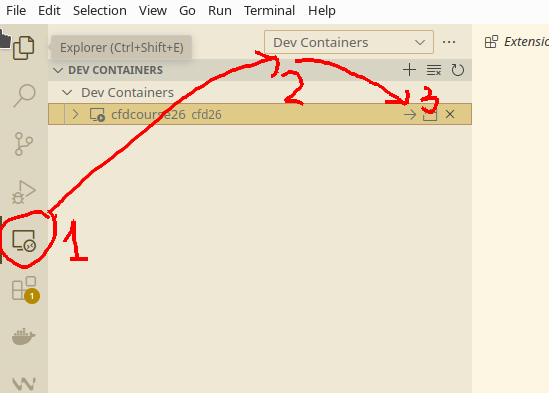
\includegraphics[width=0.6\linewidth]{attach_vscode_to_docker.png}
\caption{Подключения vscode к контейнеру}
\label{fig:vscode_to_docker}
\end{figure}

\subsubsection{Настройки vscode}
Далее необходимо открыть папку \ename{/app}: \ename{File->Open Folder...}.
Контейнер содержит в себе базовые настройки vscode, которые при сборке контейнера
копируются в папки \ename{.vscode, .vscode-server}.

Следует отметить, что удалённо подключённый vscode не может пользоваться
расширениями, установленными на хосте. Все необходимые расширения нужно устанавливать в контейнер заново.
Список базовых расширений, необходимых для работы, уже содержится в настроечных файлах.
Когда вы откроете папку \ename{app} в vscode, вам будет предложено эти расширения установить. Нужно согласиться.

Настроечные папки \ename{.vscode, .vscode-server} игнорируются системой контроля версий и расположены на хосте.
То есть вы можете дополнительно установить туда любые свои расширения и донастроить vscode как вам удобно.
Эти настройки не будут зависеть от ветки гита и не будут затираться при пересборке контейнера.

Если всё же понадобится обнулить настройки vscode, нужно
\begin{enumerate}
\item удалить папки \ename{.vscode, .vscode_server}
\item удалить все настройки из конфигурационного файла контейнера (\ename{ctrl+shift+p, open container configuration file})
\item выйти из контейнера на vscode: \ename{File->Close Remote Connection}
\item остановить и пересобрать контейнер на хосте
\begin{shelloutput}
docker stop cfd26
docker compose up --build -d
\end{shelloutput}
\end{enumerate}

\subsubsection{Сборка и отладка}
В папке \ename{.vscode} лежат базовые таски и лаунчи для компилляции и запуска программы.
В случае необходимости можете дополнить базовый набор своими командами.
Согласно настройкам по умолчанию
по нажатию \ename{F5} происходит сборка программы в отладочном режиме и запуск отладки
тестовой программы с прогоном всех тестов.
Посмотреть результаты можно на вкладке \ename{TERMINAL}.
В случае ошибок компилляции, список этих ошибок будет виден на вкладке \ename{PROBLEMS}.

Для отладки конкретного теста необходимо запустить тестовую программу с аргументом (например \cvar{cfd26_test [grid1]}.
Чтобы передать программе аргумент нужно этот аргумент прописать в файле \ename{.vscode/launch.json}
в поле \ename{args}. Либо создать ещё одну конфигурацию запуска с вашими аргументами и указать эту конфигурацию в настройке \ename{Run And Dubug}.

Чтобы собрать программу без запуска нужно выполнить таск (\ename{ctrl+shift+b}): \ename{cmake: build debug, cmake: build release}
для отладочного и релизного режима соответственно. 

В целом сборка на vscode представляет из себя автоматизированный алгоритм, представленный в п.~\ref{sec:howto_basic_dev}.
То есть исполняемая программа в дебаговой версии кладётся в папку \ename{build}, в релизной -- в \ename{build_release} и её можно запустить из терминала.
Удаление этих папок ведёт к полной очистке кэша построения.


\subsection{Работа с системой контроля версий}
Работать с гитом можно как с хоста (из папки \ename{CFDCourse26}),  так и из контейнера (из папки \ename{\app}).
Ниже будут даны инструкции для работы с гитом в консоли.
Альтернативно, можно установить графический интерфейс (например \ename{GitExtensions} для Windows)
или командами vscode на вкладке \ename{Source Control}.

Из системы контроля версий исключены следующие каталоги:
\begin{itemize}
\item build*/   -- папки со сборками,
\item .vscode, .vscode-server -- настройки и рисширения vscode,
\item local\_data -- папка для хранения любых пользовательских данных.
\end{itemize}
Изменения из этих папках не будут отслежены и скоммичены.

\subsubsection{Порядок работы с репозиторием CFDCourse}

Основная ветка проекта -- \ename{master}. После каждой лекции в эту ветку будет отправлен коммит с сообщением \ename{lect{index}}.
В этом коммите будет дополнен pdf документ с содержанием лекции, задание по итогам лекции и необходимые для этого задания изменения в коде.

\subsubsubsection{Получение последнего коммита}
Таким образом, {\bf после лекции}, после того, как изменение \ename{lect{index}} придёт на сервер, необходимо выполнить следующие команды
\begin{shelloutput}
git checkout master  # перейти на основную ветку
git pull             # получить изменения
\end{shelloutput}

Если изменения не содержали никаких изменений в настроечных файлах контейнера \ename{Dockerfile, docker-compose.yaml},
то для сборки проекта рестарт контейнера не требуется.
Иначе требуется пересобрать контейнер:
\begin{shelloutput}
docker stop cfd26            # остановить текущий контейнер
docker compose up --build -d # пересобрать новый
\end{shelloutput}

\subsubsubsection{Создание коммита с текущим дз}
{\bf Перед началом лекции}, если была сделана какая то работа по заданиям,
\begin{shelloutput}
git checkout -b hw-lect{index}      # создать локальную ветку, содержащую задание
git add .
git commit -m "{свой комментарий}"  # скоммитить свои изменения в эту ветку
\end{shelloutput}

Даже если задание выполнено не до конца, вы в любой момент можете переключиться на ветку с заданием и его доделать
\begin{shelloutput}
git checkout hw-lect{index}
\end{shelloutput}

\subsubsubsection{Создание коммита с прошлым дз}
Если вы не сделали задание вовремя и решили вернутся к нему позже, то нужно
\begin{shelloutput}
git checkout master            # перейти на основную ветку
git log --oneline              # в списке всех коммитов найти хэш коммита
                               # lect{index} той лекции которую нужно сделать
git checkout <...>             # переключиться на этот коммит по его хэшу
git checkout -b hw-lect{index} # создать ветку от этого коммита и работать в этой ветке
...                            # делаем работу
git commit -m "comment"        # по окончании работы скоммитить изменения
git checkout master            # и вернуться в основную ветку
\end{shelloutput}

\subsection{Paraview}
\label{sec:paraview}

\subsubsection{Данные на одномерных сетках}
\label{sec:paraview-1d}

Заданные на сетке данные паравью показывает цветом.
Поэтому при загрузке одномерных сеток можно видеть картинку типа
\begin{center}
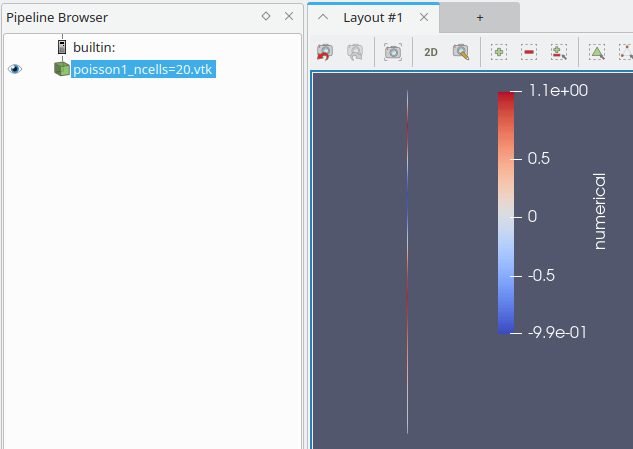
\includegraphics[width=0.5\linewidth]{howto_paraview_1d_1.png}
\end{center}
\paragraph{Развернуть изображение в плоскость xy}
\begin{center}
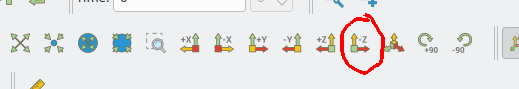
\includegraphics[width=0.5\linewidth]{howto_paraview_1d_2.png}
\end{center}
\paragraph{Отобразить данные в виде y-координаты} Для того, что бы данные отображались в качестве значения по оси ординат, к загруженному файлу необходимо
\begin{enumerate}
\item применить фильтр \ename{WarpByScalar} (В меню \ename{Filters->Alphabetical->Warp By Scalar})
\item в меню настройки фильтра указать поле данных, для отображения (numerical в примере ниже)
\item И настроить нормаль, вдоль которой будут проецироваться данные (в нашем случае ось y)
\end{enumerate}
\begin{center}
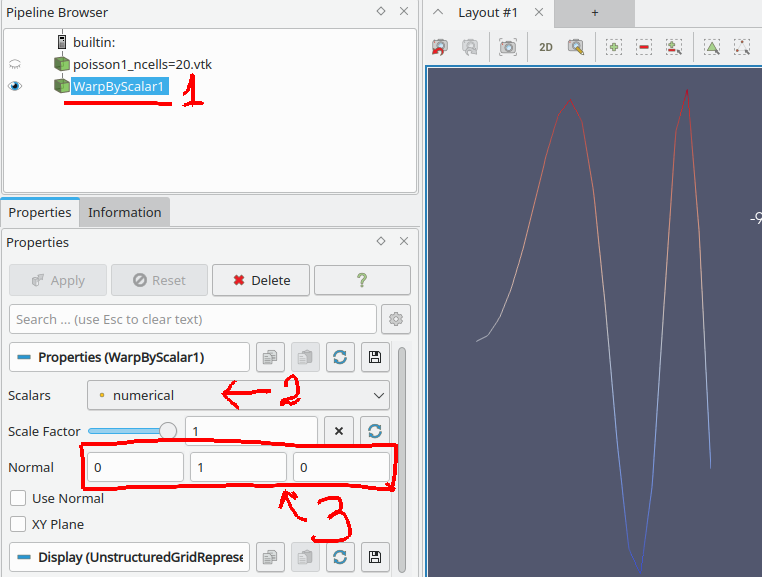
\includegraphics[width=0.5\linewidth]{howto_paraview_1d_3.png}
\end{center}

\paragraph{Цвет и толщина линии}
\begin{enumerate}
\item Включить подробные опции фильтра
\item Сменить стиль на \ename{Solid Color}
\item В меню \ename{Edit} выбрать желаемый цвет
\item В строке \ename{Line Width} указать толщину линии
\end{enumerate}
\begin{center}
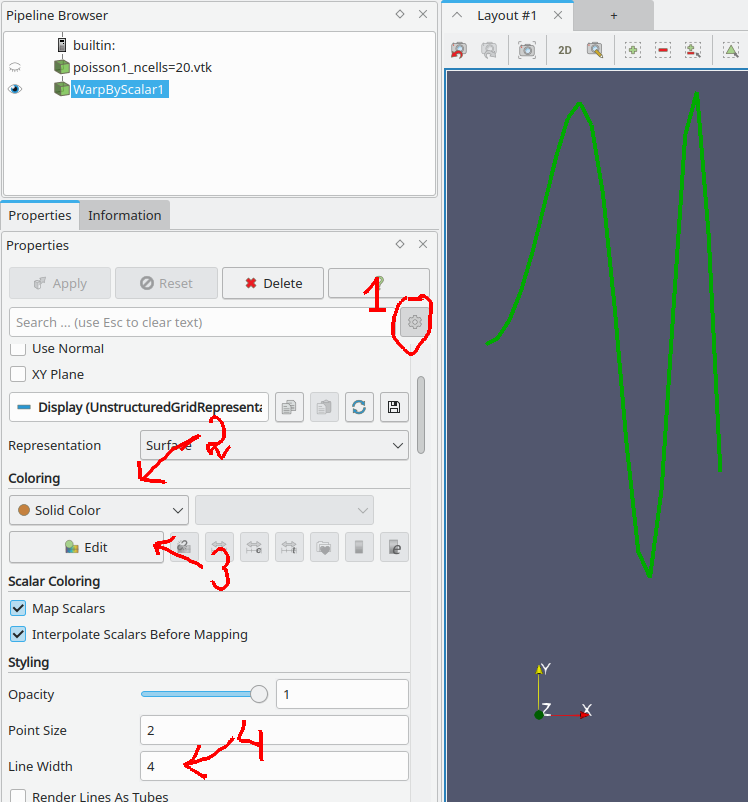
\includegraphics[width=0.6\linewidth]{howto_paraview_1d_4.png}
\end{center}

\paragraph{Настрока масштабов и отображение осей координат}
\begin{enumerate}
\item Отметье подробные настройки фильтра
\item В поле \ename{Transforming/Scale} Установите желаемые масштабы (в нашем случае растянуть в два раза по оси x)
\item Установите галку на отображение осей
\item откройте меню натройки осей
\item В нём включите подробные настроки
\item И также поставьте растяжение осей
\end{enumerate}
В случае, если масштабировать график не нужно, достаточно выполнить шаг 3.
\begin{center}
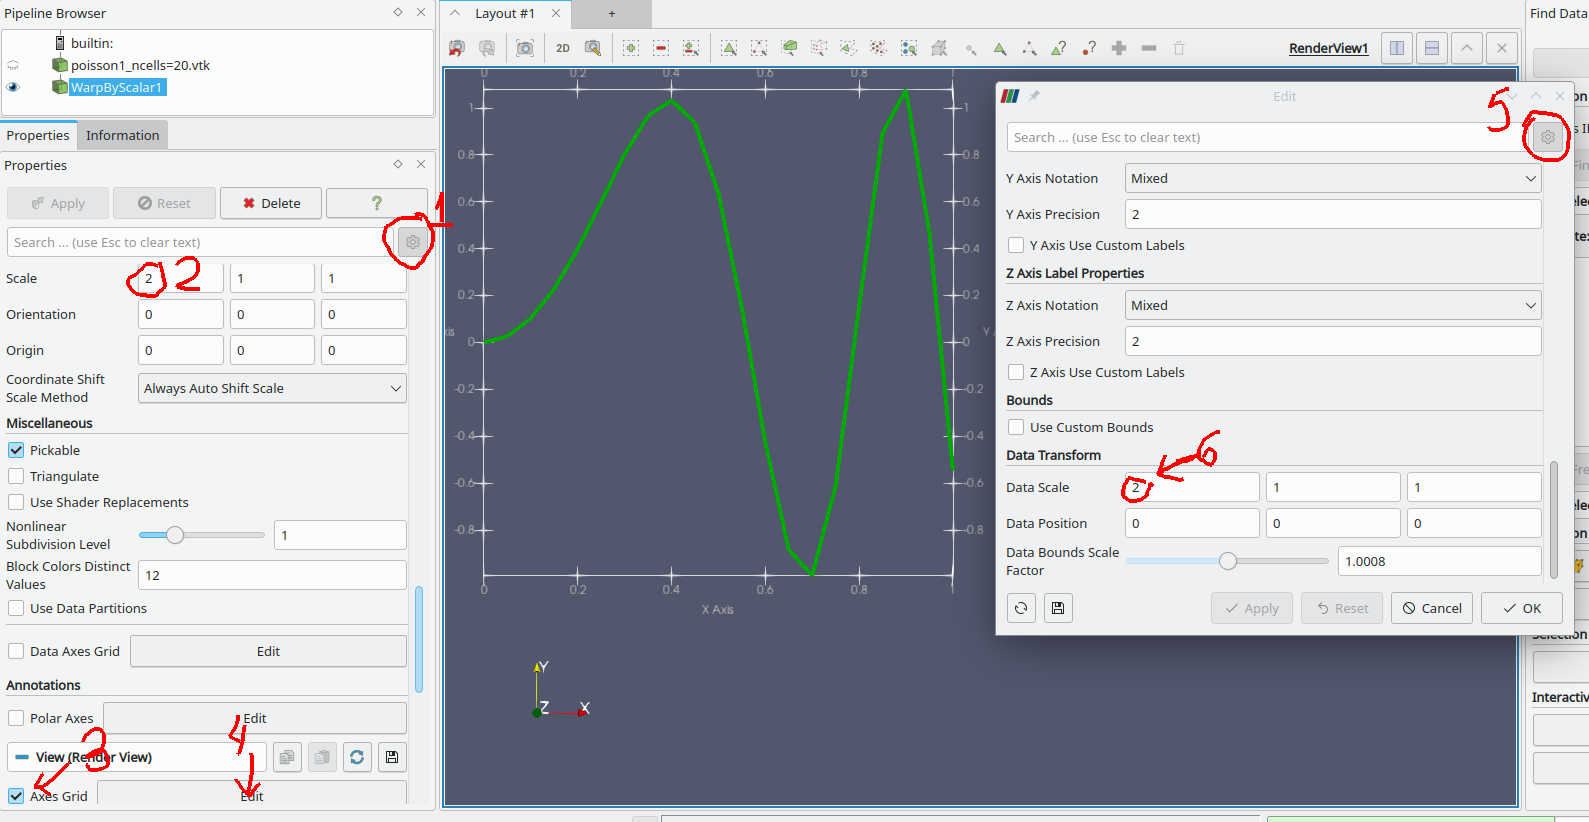
\includegraphics[width=0.9\linewidth]{howto_paraview_1d_5.png}
\end{center}

\paragraph{Построение графиков для нескольких данных}
Если требуется нарисовать рядом несколько графиков для разных данных из одного файла,
примените фильтр \ename{Warp By Scalar} для этого файла ещё раз, изменив поле \ename{Scalars} в настройке фильтра.
Для наглядности измените имя узла в Pipeline Browser на осмысленные
\begin{center}
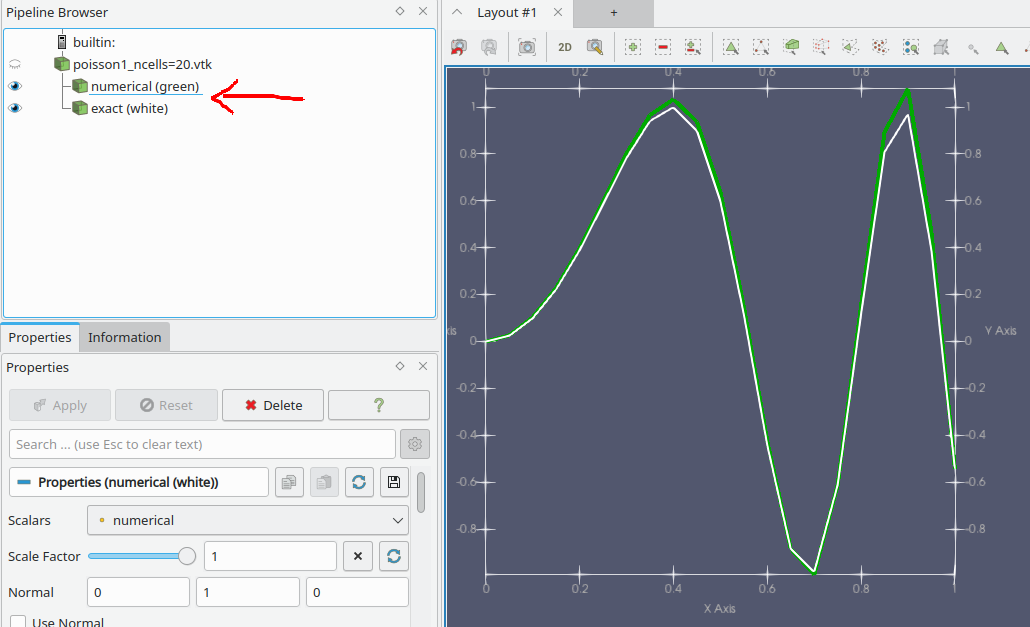
\includegraphics[width=0.8\linewidth]{howto_paraview_1d_6.png}
\end{center}

\paragraph{Обновление данных при изменении исходного файла}
В случае, если исходный файл был изменён, нужно в контекстном меню узла соответствующего файла
выбрать \ename{Reload Files} (или нажать F5). Если те же самые фильтры нужно применить для просмотра другого файла
нужно в этом меню нажать \ename{Change File}.
\begin{center}
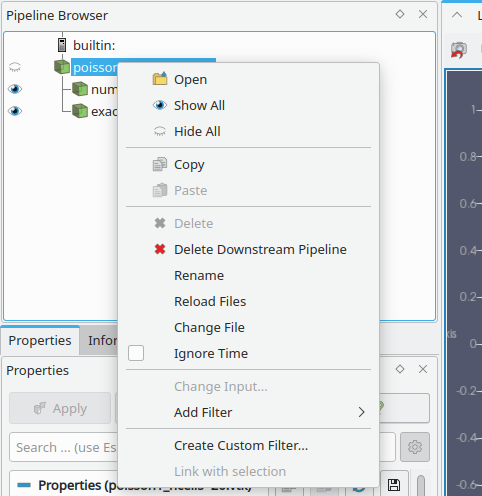
\includegraphics[width=0.4\linewidth]{howto_paraview_1d_7.png}
\end{center}

\subsubsection{Изолинии для двумерного поля}
\label{sec:paraview-isolines}

\begin{enumerate}
\item Нажмите иконку \ename{Contour} (или \ename{Filters/Contour})
      В настройках фильтра Contour by выберитее данные, по которым нужно строить изолинии.
\item В настройках фильтра удалите все существующие записи о значениях для изолиний
\item Добавьте равномерные значения. В появившемся меню установите необходимое количество изолиний и их диапазон.
\item Если необходимо, включите одновременное отображения цветного поля и изолиний.
\end{enumerate}

\begin{center}
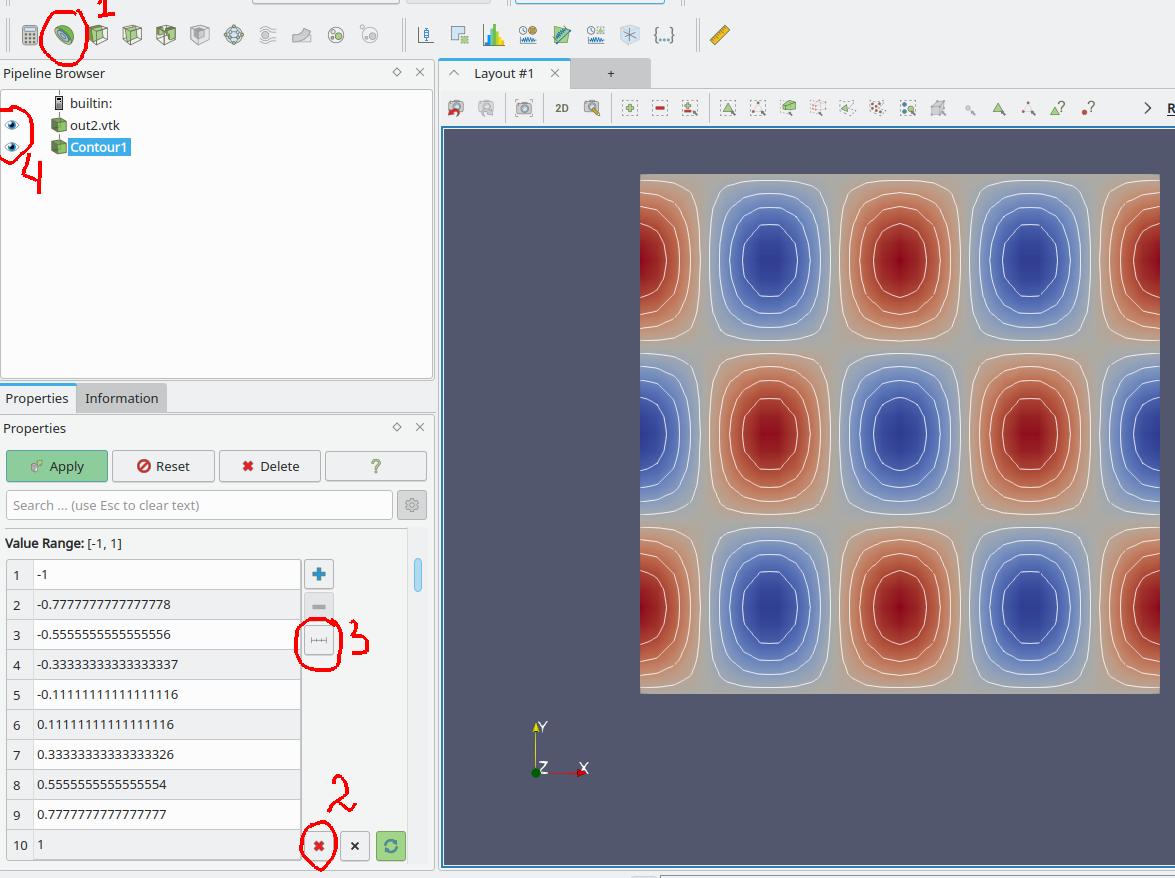
\includegraphics[width=0.7\linewidth]{howto_paraview_isolines_1.png}
\end{center}

\paragraph{Задание цвета и толщины изолинии}
В случае, если нужно сделать изолинии одного цвета, установите поле \ename{Coloring/Solid color} в 
настройках фильтра. Там же в меню \ename{Edit} можно выбрать цвет.
Для установления толщины линии включите подробные настройки и найдите там опцию \ename{Styling/Line Width}.
\begin{center}
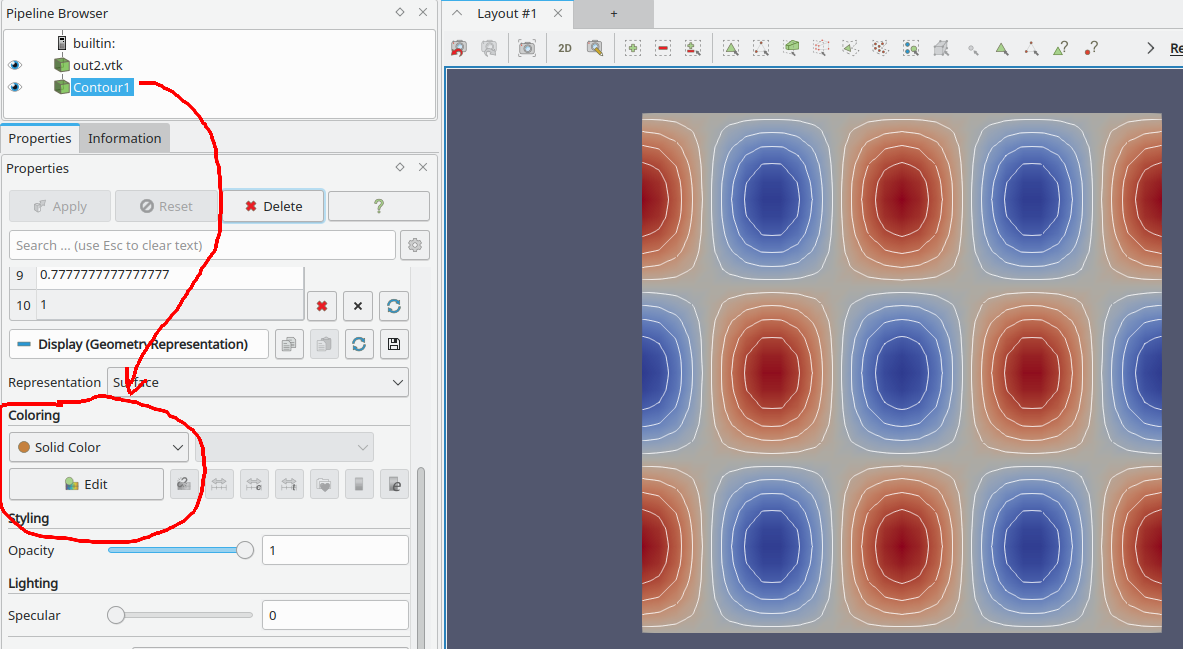
\includegraphics[width=0.7\linewidth]{howto_paraview_isolines_2.png}
\end{center}

\subsubsection{Данные на двумерных сетках в виде поверхности}
\label{sec:paraview-2d}

По аналогии с  одномерным графиком (п.~\ref{sec:paraview-1d}), двумерные поля так же
можно отобразить, проектируя данные на геометрическую координату для получения
объёмного графика. Для этого
\begin{enumerate}
\item Включите фильтр \ename{Filters/Warp By Scalar}
\item В настройках фильтра установите данные, которые будут проектироваться на координату z
\item Установите нормаль для проецирования (ось z)
\item Если нужно, выберите масштабирования для этой координаты
\item После нажатия \ename{Apply} включите трёхмерное отображение
\item Если данные не видно, обновите экран.
\end{enumerate}
\begin{center}
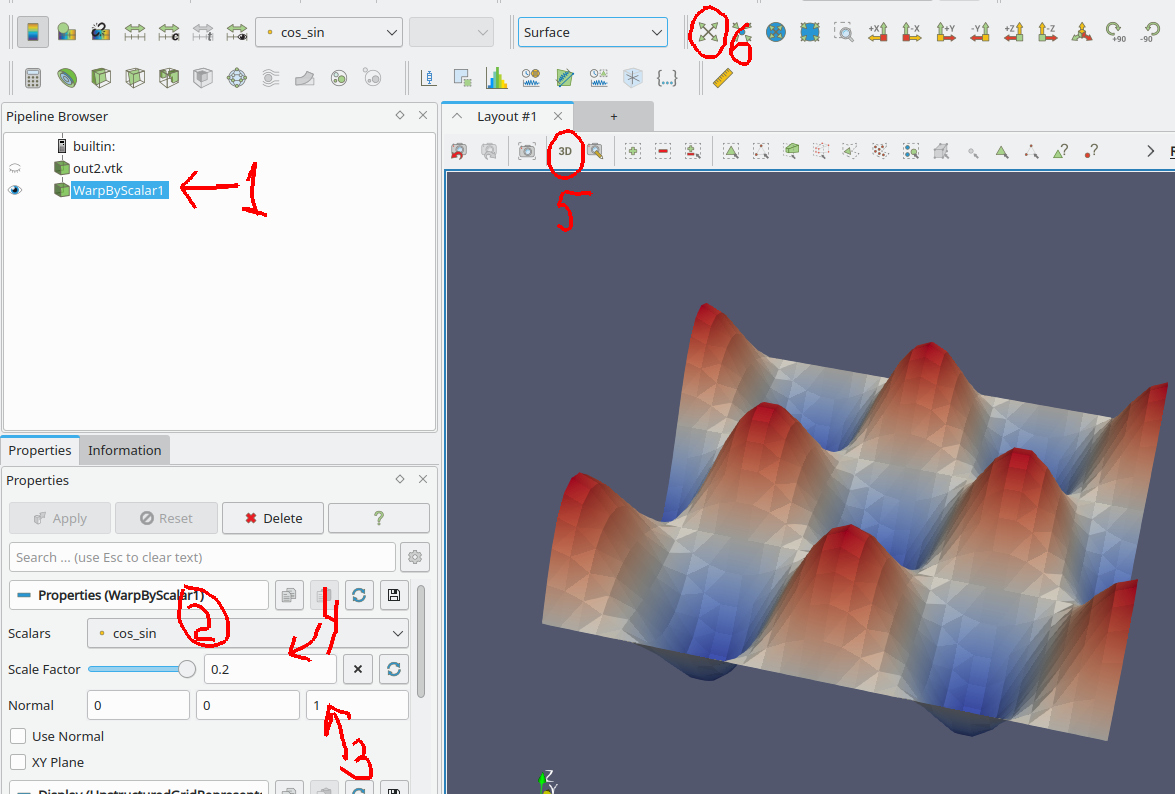
\includegraphics[width=0.9\linewidth]{howto_paraview_2d_as_3d.png}
\end{center}

\subsubsection{Числовых значения в точках и ячейках}
\label{sec:paraview-show-data}

Иногда в процессе отладки или анализа результатов расчёта
требуется знать точное значение поля в заданном узле или ячейке сетки.
Для этого

\begin{enumerate}
\item Включить режим выделения точек или ячеек (иконка (1 на рисунке) или горячие клавиши \ename{s}, \ename{d}).
      Выделить мышкой интересующую область
\item В окне \ename{Find data} (или \ename{Selection Inspector} для старых версий Paraview) отметить поле, которое должно отображаться 
      в центрах ячеек и в точках (2 на рисунке). Если такого окна нет, включить его из основного меню \ename{View}.
\end{enumerate}

\begin{center}
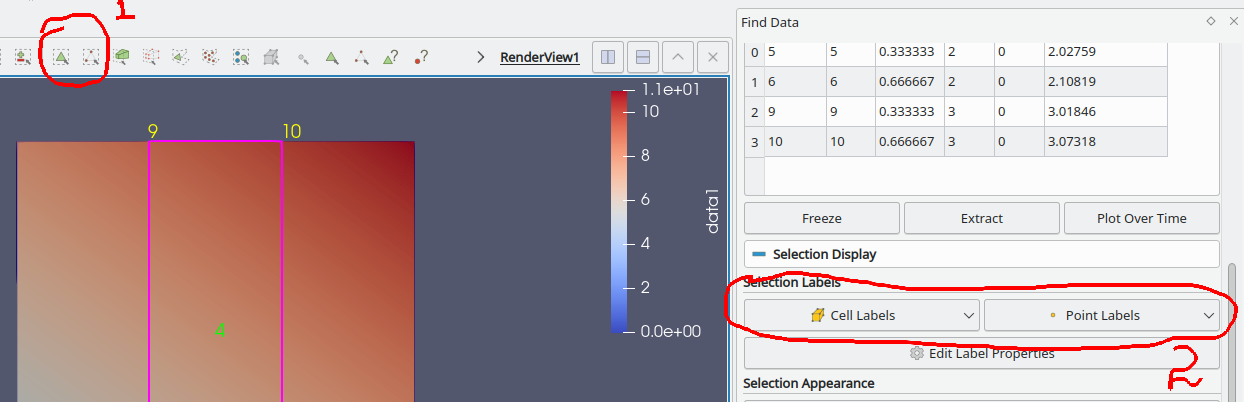
\includegraphics[width=0.8\linewidth]{howto_paraview_show_labels.png}
\end{center}

\subsubsection{Векторные поля}
\label{sec:paraview-glyph}

Открыть файл vtk или vtk.series, который содержит
векторное поле. Далее
\begin{enumerate}
\item Создать фильтр \ename{Glyph}
\item Задать двумерный тип стрелки
\item Сместить центр стрелки, чтобы она исходила из точки, к которой приписана
\item Отметить необходимое векторное поле в качестве ориентации
\item Отметить необходимое векторное поле для масштабирования
      Нажать \ename{Apply}.
\end{enumerate}

\begin{center}
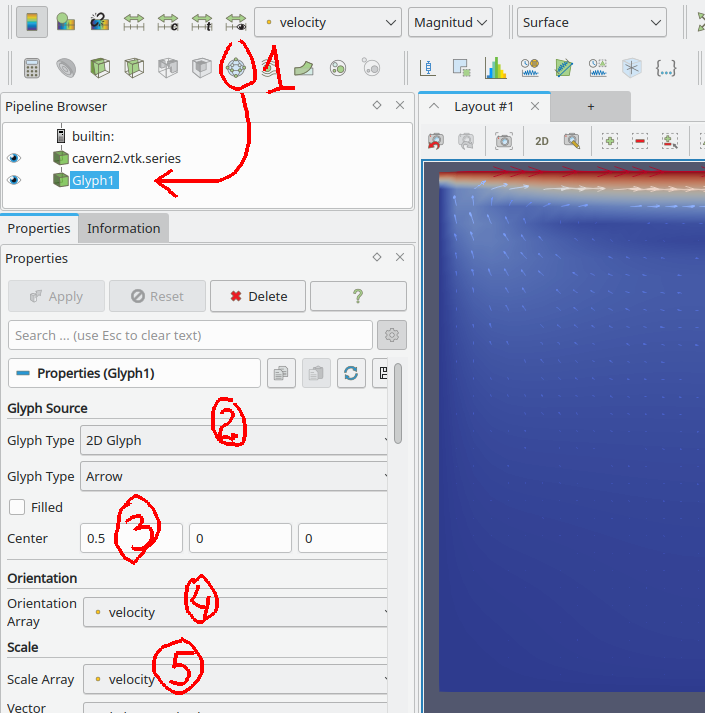
\includegraphics[width=0.6\linewidth]{glyph-1.png}
\end{center}

\paragraph{Настройка отображения стрелок}
\begin{enumerate}
\item Выбрать необходимый \ename{Glyph-mode}. Если сетка небольшая, то можно \ename{All Points}.
\item Установить белый цвет для стрелок. Нажать Apply.
\end{enumerate}

\begin{center}
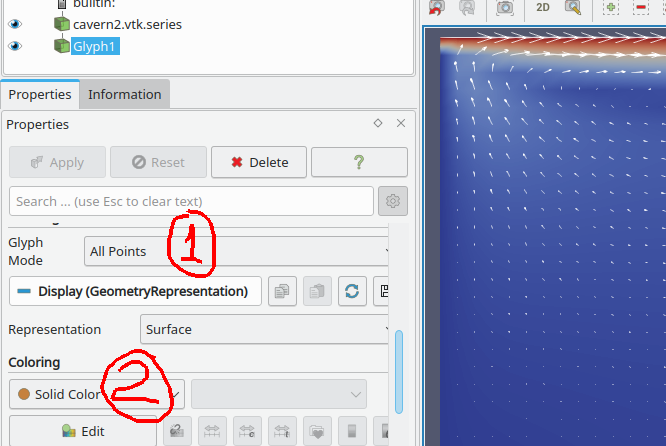
\includegraphics[width=0.4\linewidth]{glyph-2.png}
\end{center}

\paragraph{Уменьшения разброса по длине стрелок}
Если разброс по длинам стрелок слишком велик, его можно подравнять,
введя новую функцию $|\vec v|^{\alpha}$ -- длина вектора в степени меньше единицы (например, $\alpha=0.7$).
Такую функцию можно создать через калькулятор

\begin{enumerate}
\item Начиная от загруженного файла создать фильтр \ename{Calculator}
\item Там вбить необходимую формулу
\end{enumerate}
\begin{center}
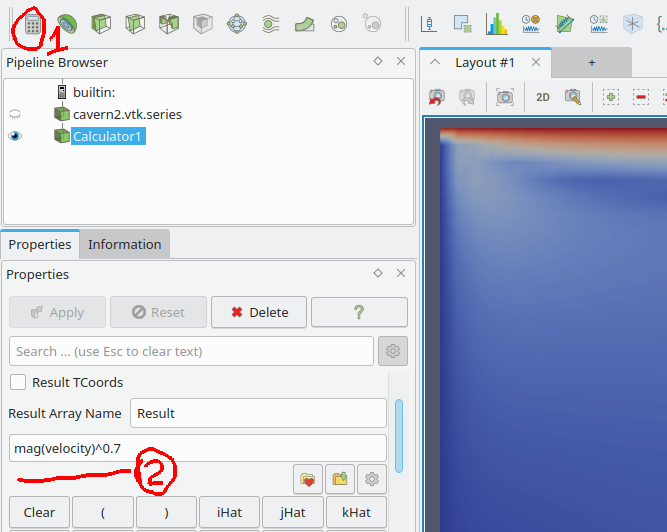
\includegraphics[width=0.6\linewidth]{glyph-3.png}
\end{center}
Созданную функцию нужно прокинуть в \ename{Glyph} в качестве коэффициента масштабирования
\begin{enumerate}
\item В \ename{Scale Array} фильтра \ename{Glyph} указать уже результат работы \ename{Calculator}-a (\ename{Result} по умолчанию),
\item Подтянуть значение \ename{Scale Factor} до приемлимого
\item Не забыть отключить вспомогательное поле \ename{Calculator} из отображения
\end{enumerate}
\begin{center}
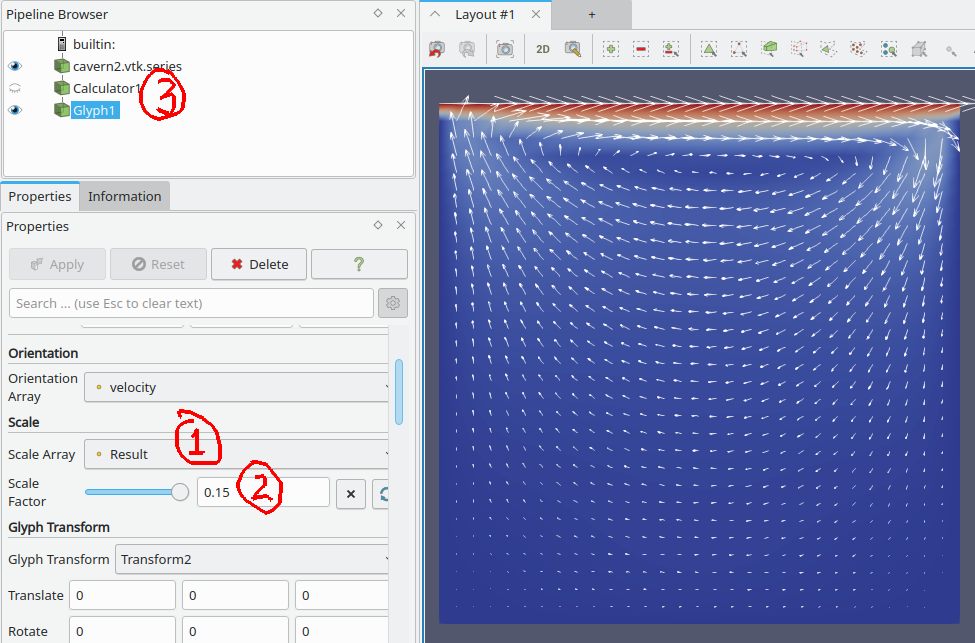
\includegraphics[width=0.6\linewidth]{glyph-4.png}
\end{center}

\subsubsection{Значение функции вдоль линии}
\label{sec:paraview-plot-over-line}

\begin{enumerate}
\item
Выбрать фильтр \ename{Plot Over Line} иконкой или в меню \ename{Filters}
\item
Установить начальную и конечную точку сечения
\item
Можно использовать привязку к узлам сетки с помощью горячих клавиш (в подсказках написано)
\item
Можно установить координаты руками в соответствующем поле. Для двумерных задач проследить,
что координата Z равна нулю
\item
Нажать \ename{Apply}
\end{enumerate}

\begin{center}
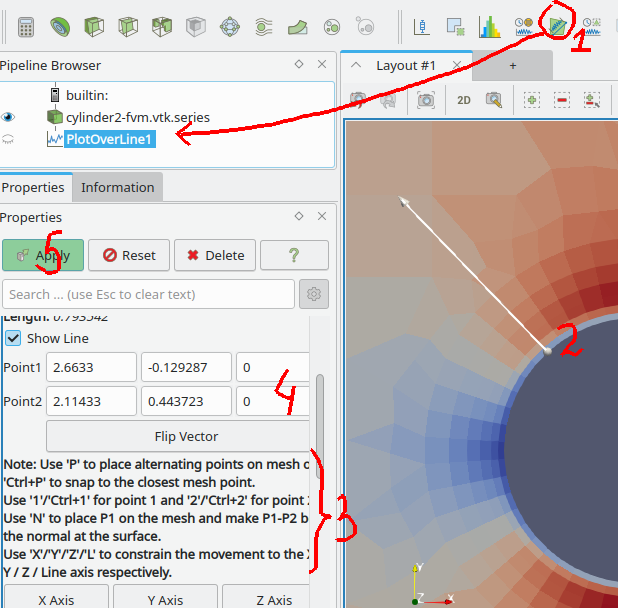
\includegraphics[width=0.4\linewidth]{howto_paraview_plot_over_line_1.png}
\end{center}

\paragraph{Настройка графика}
\begin{enumerate}
\item
После установок появится дополнительное окно типа \ename{Line Chart View} с нарисованным графиком.
\item
Сделав это окно активным в настройках фильтра \ename{PlotOverLine}
можно выбрать, какие поля рисовать (\ename{Series Parameters})
\end{enumerate}

\begin{center}
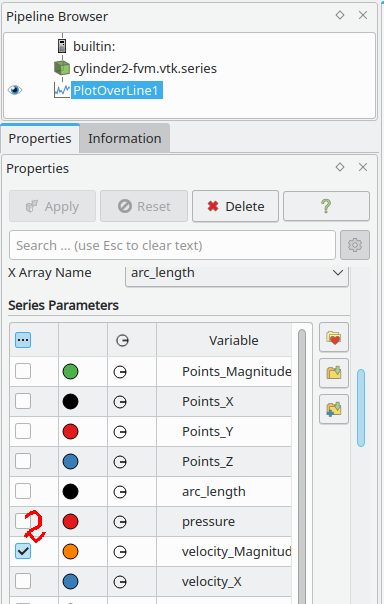
\includegraphics[width=0.2\linewidth]{howto_paraview_plot_over_line_3.png}
\quad
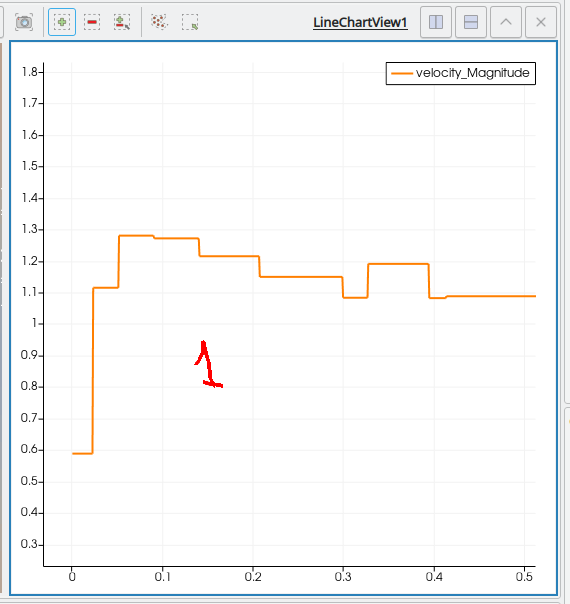
\includegraphics[width=0.3\linewidth]{howto_paraview_plot_over_line_2.png}
\end{center}

\paragraph{Отрисовка в отдельном окне}
\begin{enumerate}
\item
Открыть новую вкладку
\item
Выбрать \ename{Line Chart View}
\item
Выбрать предварительно созданный фильтр с одномерным графиком
\end{enumerate}
\begin{center}
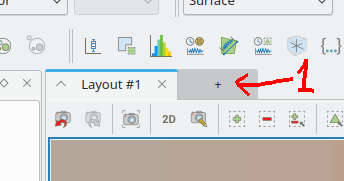
\includegraphics[width=0.2\linewidth]{howto_paraview_plot_over_line_4.png}
\quad
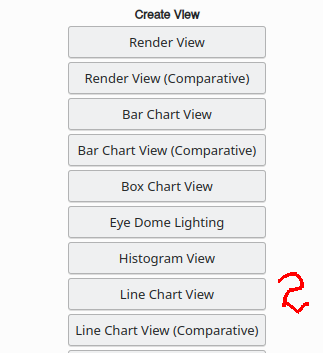
\includegraphics[width=0.3\linewidth]{howto_paraview_plot_over_line_5.png}
\quad
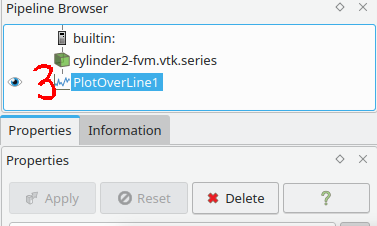
\includegraphics[width=0.3\linewidth]{howto_paraview_plot_over_line_6.png}
\end{center}

\subsection{Hybmesh}
\label{sec:hybmesh}

Генератор сеток на основе композитного подхода.
Работает на основе python-скрипотов.
Полная документация \url{http://kalininei.github.io/HybMesh/index.html}

\subsubsection{Работа в Windows}
Инсталлятор программы следует скачать по ссылке
\url{https://github.com/kalininei/HybMesh/releases}
и установить стандартным образом.

Для запуска скрипта построения \ename{script.py} нужно
открыть консоль, перейти в папку с нужным скриптом,
оттуда выполнить (при условии, что программа была установлена в папку \ename{C:\Program Files}):
\begin{shelloutput}
> "C:\Program Files\HybMesh\bin\hybmesh.exe" -sx script.py
\end{shelloutput}

\subsubsection{Работа в Linux}
Версию для линукса нужно собирать из исходников.
Либо, если собрать не получилось,
можно строить сетки в Windows и переносить
полученные vtk-файлы на рабочую систему. 

Перед сборкой в систему необходимо установить dev-версии
пакетов \ename{suitesparse} и \ename{libxml2}. Также 
должны быть доступны компилляторы \ename{gcc-c++} и \ename{gcc-fortan} и \ename{cmake}.
Программа работает со скиптами python2.
Лучше установить среду anaconda (\url{https://docs.anaconda.com/free/anaconda/install/index.html})
И в ней создать окружение c python-2.7:
\begin{shelloutput}
> conda create -n py27 python=2.7   # создать среду с именем py27
> conda activate py27               # активировать среду py27
> pip install decorator             # установить пакет decorator
\end{shelloutput}

Сначала следует склонировать репозиторий в папку с репозиториями гита:
\begin{shelloutput}
> cd D:/git_repos
> git clone https://github.com/kalininei/HybMesh
\end{shelloutput}

Поскольку программа не предназначена для запуска из под анаконды,
в сборочные скрипты нужно внести некоторые изменения.
В корневом сборочном файле \ename{HybMesh/CMakeLists.txt} 
нужно закомментировать все строки в диапазоне
\begin{minted}[linenos=false]{text}
# ========================== Python check
....
# ========================== Windows installer options
\end{minted}
а в файле \ename{HybMesh/src/CMakeLists.txt} последнюю строку
\begin{minted}[linenos=false]{text}
#add_subdirectory(bindings)
\end{minted}

Далее, находясь в корневой директории репозитория HybMesh, запустить сборку
\begin{shelloutput}
> mkdir build
> cd build
> cmake .. -DCMAKE_BUILD_TYPE=Release
> make -j8
> sudo make install
\end{shelloutput}

Для запуска скриптов нужно создать скрипт-прокладку
\begin{minted}[linenos=false]{python}
import sys
sys.path.append("/path/to/HybMesh/src/py/")  # вставить полный путь к Hybmesh/src/py
execfile(sys.argv[1])
\end{minted}
и сохранить его в любое место. Например в \ename{path/to/HybMesh/hybmesh.py}.

Для запуска скрипта построения сетки следует перейти в папку, где находится нужный скрипт \ename{script.py},
убедится, что анаконда работает в нужной среде (то есть \ename{conda activate py27} был вызван),
и запустить
\begin{shelloutput}
> python /path/to/HybMesh/hybmesh.py script.py
\end{shelloutput}


\end{document}
